% Konfigurationsdatei f\"ur die Pfaddefinitionen einlesen
%  se-wa-pfade.tex
%
%
%  J\"org Baumgart
%  2012-12-20
%  
%  Pfaddefinitionen (Ordnerdefinitionen) f\"ur das Einlesen von
%  -- .sty-Dateien und
%  -- Textbaustenen f\"ur die Hinweise zur Verwendung von LaTeX
%  -- jpg-Bildern
%
\newcommand{\seWaPathSty}{se-wa-styles}
\newcommand{\seWaPathText}{se-wa-textbausteine-vorlagen}
\newcommand{\seWaPathJpg}{images}

%
%
% Festlegung der Sprache: 
\newcommand{\seWaSprache}{deutsch}
%\newcommand{\seWaSprache}{englisch}

%
% Einlesen der .sty-Dateien
%
%  se-wa-input-styles-v098.tex
%
%  Joerg Baumgart 01.08.2011
%
%  Zusammenfassung und Konfiguration wichtiger Styles f\"ur die 
%  Erzeugung von Seminar-, Projekt- und Bachelorarbeiten
%
%  2012-03-12: auf Version 0.94 umgestellt
%
%
% 2012-12-13: auf Version 0.95 umgestellt
%                     Sprachoptionen englisch/deutsch zusammengef\"uhrt
%                     bchart.sty hinzugenommen
%                 
%
% 2013-01-27: auf Version 0.96 umgestellt
%                     algorithm2e-Paket integriert
%
%
% 2013-07-08: auf Version 0.97 umgstellt 
%                     utf8, Fehlerkorrekturen bei pa1
%
% 2014-02-02: auf Version 0.971 umgestellt
%                     Workaround für Fehler im KOMAScript 3.2
%                     KOMAoption listof un documentclass übernommen
%
%
%
%
% 2014-07-22: etex-Paket hinzugenommen
%
%
% 2016-04-01: Sperrvermerk und Ehrenwörtliche Erklärung aus der PO 2015
%
%
%
% 2016-12-18: auf Version 0.98 umgestellt
%                     bchart.sty und algorithm2e haben veraltete Kommandos verwendet (\sf und \bf), 
%                     die unter MacTeX 2016 nicht mehr unterstützt werden 
%

\documentclass[12pt,BCOR=10mm,headinclude=on,footinclude=off,bibliography=totoc,listof=ignorechapter]{scrreprt}
\usepackage{etex}
\usepackage[T1]{fontenc}
\usepackage[utf8]{inputenc}
\usepackage{ifthen}
% 2012-12-13
\ifthenelse{\equal{\seWaSprache}{deutsch}}{% Deutsche Einstellungen
\usepackage[ngerman]{babel}% 
}{% Englische Einstellungen
\usepackage[english]{babel}% 
}

\usepackage{lmodern}

\usepackage{tikz} % Graphikpaket, das zu pdfLaTeX kompatibel ist
\usepackage{xkeyval} % Definition von Kommandos mit mehreren optionalen Argumenten
\usepackage{listings} % Formatierung von Programmlistings
\usepackage{graphicx} % Einbinden von Graphiken
\usepackage{color}
\usepackage{\seWaPathSty/slashbox} % Diagonalen in Tabellenfeldern
\usepackage{framed} % Erzeugung schwarzer Linien am linken Rand zur Hervorhebung von Textteilen
\usepackage{caption} % Korrektes Setzen einer mehrzeiligen float-Unterschrift bei neu definierten float-Umgebungen
\usepackage{floatrow}
% 2012-12-13
\usepackage{\seWaPathSty/bchart} % Kommandos zur Erzeugung von Balkendiagrammen
% 2013-01-27 
\usepackage[boxed,ngerman]{\seWaPathSty/algorithm2e}
%\usepackage[tworuled,vlined,ngerman]{\seWaPathSty/algorithm2e}


% Es wird jeweils die sty-Datei importiert und entsprechende Konfigurationseinstellungen werden vorgenommen

\usepackage{\seWaPathSty/se-jb-scrpage2} % Formatierung der Kopf- und Fu{\ss}zeilen
\usepackage{\seWaPathSty/se-jb-footmisc}    % Fussnoten besser formatieren

\usepackage{\seWaPathSty/se-jb-glossaries-v097} % Abk\"urzungsverzeichnis, Symbolverzeichnis, Glossar
   
\usepackage{\seWaPathSty/se-jb-floatrow}    % Definition und Konfiguration von float-Umgebungen (figure, table, die neue programm-Umgebung)
% Achtung: se-jb-varioref muss nach se-jb-floatrow importiert werden; 
% andernfalls ist der counter programm f\"ur die labelformat-Anweisung noch nicht definiert   
\usepackage{\seWaPathSty/se-jb-varioref-v097}   % Definition von Querverweisen
\usepackage{\seWaPathSty/se-jb-chngcntr}   % Kapitelweise oder globale Nummerierung von Abbildungen etc.
   
\usepackage{\seWaPathSty/se-jb-listen} % Definition neuer, besser formatierter Listen
% 2014-02-02
%\usepackage{\seWaPathSty/se-jb-kommandos-v097} % neue Kommandos f\"ur Seminar-, Projekt- und Bachelorarbeiten
%\usepackage{\seWaPathSty/se-jb-kommandos-v0971} % neue Kommandos f\"ur Seminar-, Projekt- und Bachelorarbeiten
% 2016-04-01
\usepackage{\seWaPathSty/se-jb-kommandos-v0972} % neue Kommandos f\"ur Seminar-, Projekt- und Bachelorarbeiten
% 2012-12-13
\ifthenelse{\equal{\seWaSprache}{englisch}}{\usepackage{\seWaPathSty/se-jb-kommandos-englisch-v0972}}{}

% 2016-12-18
\renewcommand{\sf}{\sffamily}
\renewcommand{\bf}{\bfseries}




%
% Individuelle Konfiguration des Dokumentes
%
%  Individuelle Konfiguration einer Projektarbeit/Bachelorarbeit
%
%
%
%

% 2012-10-27
%
% \"Anderung des Schrifttyps f\"ur das gesamte Dokument
%
% Das gesamte Dokument wird in einer serifenlosen Schrift gesetzt
%\renewcommand{\familydefault}{\sfdefault}
%
% Das gesamte Dokument wird in einer Serifenschrift gesetzt
% Achtung: serifenlose Schriften sind jetzt grunds\"atzlich nicht mehr nutzbar!
%
%\renewcommand{\sffamily}{\normalfont}

% 2012-12-05
%
% Verwendung des url-Pakets
% Durch den optionalen Paremeter hyphens wird eine Trennung 
% von URLs auch nach Bindestrichen erlaubt
\usepackage[hyphens]{url}


% 2012-10-27
%
%
% Literaturverzeichnis
% 
% Literaturverzeichnis gem\"ass den Vorgaben von Theisen aufbauen
\usepackage{\seWaPathSty/se-jb-jurabib-theisen} 
% Verwendung der Harvard-Zitierweise
%\usepackage{\seWaPathSty/se-jb-jurabib-harvard} 

% Weitere Optionseinstellungen f\"ur das Koma-Script
%
% Zwischen Abs\"atzen einen Abstand von 0.5 \baselineskip erzeugen
\KOMAoption{parskip}{full}
%
% Vergleiche Duden "Gliederung von Nummern, S.111" 
% DIN 5008 anschauen, wenn sie neu ver\"offentlicht wurde
\KOMAoption{numbers}{noendperiod}
%
%



%  Voreinstellungen f\"ur floats
%  Durch die verwendeten Parameter wird die Wahrscheinlichkeit deutlich kleiner, 
%  dass Gleitobjekte (z. B. Abbildungen) ans Ende des Dokumentes verschoben 
%  werden; 
%  Achtung: clearpage erzwingt die Ausgabe von Gleitobjekten
%
\renewcommand{\topfraction}{1}  % Gleitobjekte d\"urfen eine Seite zu 100% belegen 
\renewcommand{\bottomfraction}{1} % Entsprechender Wert f\"ur den unteren Teil der Seite
\renewcommand{\textfraction}{0} % Eine Seite darf auch ohne Fliesstext existieren
%%%\renewcommand{\floatpagefraction}{1} % Bedeutung unklar, daher keine Ver\"anderung des Vorgabewertes 
                                                                        % von 0.5; eventuell bringt ein \"Anderung auf 1 etwas, wenn 
                                                                         % Probleme mit floats auftreten
                                                                         
                                                                         
                                                                         
% Konfiguration von Programm-Listings
% 
% Achtung: hier gibt es nahezu beliebig viele weitere Konfigurationm\"oglichkeiten; vgl. Paketdokumentation
%
\lstset{language=Java,basicstyle=\ttfamily,keywordstyle=\color{blue},captionpos=b,aboveskip=0mm,belowskip=0mm,
          xleftmargin=0em}               
          
%
% Grundkonfiguration der Abs\"ande zwischen den Items der maximal f\"unf Verschachtelungsebenen der 
% neuen Listenumgebungen
%                                                                             
% Initialisierung der Abst\"ande zwischen den items f\"ur seList; Grundeinheit: 0.5\baselineskip; siehe se-jb-listen
\seSetlistbaselineskip{1}{0.75}{0.75}{0.75}{0.75}
% Initialisierung der Abst\"ande zwischen den items f\"ur seToplist; Grundeinheit: 0.5\baselineskip; siehe se-jb-listen
\seSettoplistbaselineskip{1}{0.75}{0.75}{0.75}{0.75}     


% Einlesen der sprachabh\"angigen Konfigurationsdatei
%
%
\ifthenelse{\equal{\seWaSprache}{deutsch}}{% deutsch
% wa-konfiguration-deutsch
%
% 2012-12-13
% 
% Diese Datei wird f\"ur die Sprachoption deutsch verwendet, d. h.  
% \newcommand{\seWaSprache}{deutsch}
%
%
% In dieser Datei k\"onnen Neudefinitionen vorgenommen werden f\"ur:
% -- Verzeichnisse
% -- Unter-/\"Uberschriften von Abbildungen, Tabellen und Listings
% -- Querverweise innerhalb des Textes

% 2013-01-26: Konfiguration des Algorithmenverzeichnis
%
%
%

% 2013-07-08: Querverweis auf Anhang hinzugenommen
%
%
%


%
%  Konfiguration der verschiedenen Verzeichnisse
%
%  abstandEintrag: Wert wird mit \baselineskip multipliziert
%

%
%  Abbildungsverzeichnis
%
\seKonfigurationAbb[
%verzeichnisname=Abbildungsverzeichnis,
labeltextLinks=, % kein Text links;
%labeltextRechts=:,
labelbreite=1cm,
%labeleinzug=1cm,
%abstandEintrag=1,
%newpage=ja,
%pnumwidth=20mm,
%dotsep=1000,
%tocrmarg=4.5cm,
%abstandVerzeichnis=-1mm
]

%
% LIstingverzeichnis
%
\seKonfigurationPrg[
%verzeichnisname=Listing-Verzeichnis,
labeltextLinks=,
%labeltextRechts=:,
labelbreite=1cm,
%labeleinzug=2cm,
%abstandEintrag=1,
%newpage=ja,
%pnumwidth=20mm,
%dotsep=1000,
%tocrmarg=4.5cm,
%abstandVerzeichnis=-10mm
]

% 2013-01-26
%
% Algorithmenverzeichnis
%
\seKonfigurationAlg[
%verzeichnisname=Algorithmen-Verzeichnis,
labeltextLinks=,
%labeltextRechts=:,
labelbreite=1cm,
%labeleinzug=2cm,
%abstandEintrag=1,
%newpage=ja,
%pnumwidth=20mm,
%dotsep=1000,
%tocrmarg=4.5cm,
%abstandVerzeichnis=-10mm
]




%
% Tabellenverzeichnis
%
\seKonfigurationTab[
%verzeichnisname=Liste der Tabellen,
labeltextLinks=,
%labeltextRechts=:,
labelbreite=1cm,
%labeleinzug=0.5cm,
%abstandEintrag=1,
%newpage=ja,
%pnumwidth=20mm,
%dotsep=1000,
%tocrmarg=4.5cm,
%abstandVerzeichnis=-10mm
]

%
% Abk\"urzungsverzeichnis
%
\seKonfigurationAbk[
%verzeichnisname=Liste der Abk\"urzungen,
%labelbreite=3cm,
%labeleinzug=0.5cm,
%abstandEintrag=1,
%newpage=ja,
%abstandVerzeichnis=-10mm
]

%
% Symbolverzeichnis
% 
\seKonfigurationSym[
%verzeichnisname=Liste der Symbole,
%labelbreite=4cm,
%labeleinzug=3.5cm,
%abstandEintrag=1,
%newpage=ja,
%abstandVerzeichnis=-10mm
]

%
% Glossar
%
\seKonfigurationGlo[
%verzeichnisname=Glossar,
%abstandEintrag=0,
]



% (eventuelle) Neudefinition f\"ur die Unter-/\"Uberschriften von Abbildungen, Tabellen und Listings
%
%
%\renewcommand{\seCaptionNameAbbildung}{Abb.}
%\renewcommand{\seCaptionNameTabelle}{Tab.}
%\renewcommand{\seCaptionNameProgramm}{Prg.}


% % (eventuelle) Neudefinition f\"ur Querverweise innerhalb des Textes
%
%
%
%\renewcommand{\seQuerverweisSeite}{Seite}
%\renewcommand{\seQuerverweisAbbildung}{Abb.}
%\renewcommand{\seQuerverweisTabelle}{Tab.}
%\renewcommand{\seQuerverweisProgramm}{Prg.}
%\renewcommand{\seQuerverweisGleichung}{Gl.}
%\renewcommand{\seQuerverweisAlgorithmus}{Alg.}
%
\renewcommand{\seQuerverweisChapter}{Kapitel}
% 2013-07-08
\renewcommand{\seQuerverweisAppendix}{Anhang}
\renewcommand{\seQuerverweisSection}{Kapitel}
\renewcommand{\seQuerverweisSubsection}{Kapitel}
\renewcommand{\seQuerverweisSubsubsection}{Kapitel}
\renewcommand{\seQuerverweisParagraph}{Kapitel}


%
% Kommandos f\"ur die Konfiguration von URL-Eintr\"agen im Literaturverzeichnis
%
\renewcommand*{\biburlprefix}{\jblangle{}URL: }
\renewcommand*{\biburlsuffix}{\jbrangle{}}
\renewcommand*{\bibbudcsep}{ -- }
\AddTo\bibsgerman{\renewcommand*{\urldatecomment}{Zugriff am }}


%
}{% englisch
% wa-konfiguration-englisch
%
% 2012-12-13
% 
% Diese Datei wird f\"ur die Sprachoption englisch verwendet, d. h.  
% \newcommand{\seWaSprache}{englisch}
%
%
% In dieser Datei k\"onnen Neudefinitionen vorgenommen werden f\"ur:
% -- Verzeichnisse
% -- Unter-/\"Uberschriften von Abbildungen, Tabellen und Listings
% -- Querverweise innerhalb des Textes

% 2013-07-08: Querverweis auf Anhang hinzugenommen
%
%
%


%
%  Konfiguration der verschiedenen Verzeichnisse
%
%  abstandEintrag: Wert wird mit \baselineskip multipliziert
%

%
%  Abbildungsverzeichnis
%
\seKonfigurationAbb[
verzeichnisname=List of Figures,
labeltextLinks=, % kein Text links;
%labeltextRechts=:,
labelbreite=1cm,
%labeleinzug=1cm,
%abstandEintrag=1,
%newpage=ja,
%pnumwidth=20mm,
%dotsep=1000,
%tocrmarg=4.5cm,
%abstandVerzeichnis=-1mm
]

%
% LIstingverzeichnis
%
\seKonfigurationPrg[
verzeichnisname=List of Program Listings,
labeltextLinks=,
%labeltextRechts=:,
labelbreite=1cm,
%labeleinzug=2cm,
%abstandEintrag=1,
%newpage=ja,
%%pnumwidth=20mm,
%dotsep=1000,
%tocrmarg=4.5cm,
%abstandVerzeichnis=-10mm
]


% 2013-01-26
%
% Algorithmenverzeichnis
%
\seKonfigurationAlg[
verzeichnisname=List of Algorithms,
labeltextLinks=,
%labeltextRechts=:,
labelbreite=1cm,
%labeleinzug=2cm,
%abstandEintrag=1,
%newpage=ja,
%pnumwidth=20mm,
%dotsep=1000,
%tocrmarg=4.5cm,
%abstandVerzeichnis=-10mm
]


%
% Tabellenverzeichnis
%
\seKonfigurationTab[
verzeichnisname=List of Tables,
labeltextLinks=,
%labeltextRechts=:,
labelbreite=1cm,
%labeleinzug=0.5cm,
%abstandEintrag=1,
%newpage=ja,
%pnumwidth=20mm,
%dotsep=1000,
%tocrmarg=4.5cm,
%abstandVerzeichnis=-10mm
]

%
% Abk\"urzungsverzeichnis
%
\seKonfigurationAbk[
verzeichnisname=List of Abbreviations,
%labelbreite=3cm,
%labeleinzug=0.5cm,
%abstandEintrag=1,
%newpage=ja,
%abstandVerzeichnis=-10mm
]

%
% Symbolverzeichnis
% 
\seKonfigurationSym[
verzeichnisname=List of Symbols,
%labelbreite=4cm,
%labeleinzug=3.5cm,
%abstandEintrag=1,
%newpage=ja,
%abstandVerzeichnis=-10mm
]

%
% Glossar
%
\seKonfigurationGlo[
verzeichnisname=Glossary,
%abstandEintrag=0,
]



% (eventuelle) Neudefinition f\"ur die Unter-/\"Uberschriften von Abbildungen, Tabellen und Listings
%
%
\renewcommand{\seCaptionNameAbbildung}{Figure}
\renewcommand{\seCaptionNameTabelle}{Table}
\renewcommand{\seCaptionNameProgramm}{Listing}
\renewcommand{\seCaptionNameAlgorithmus}{Algorithm}


% % (eventuelle) Neudefinition f\"ur Querverweise innerhalb des Textes
%
%
%
\renewcommand{\seQuerverweisSeite}{page}
\renewcommand{\seQuerverweisAbbildung}{figure}
\renewcommand{\seQuerverweisTabelle}{table}
\renewcommand{\seQuerverweisProgramm}{listing}
\renewcommand{\seQuerverweisGleichung}{equation}
\renewcommand{\seQuerverweisAlgorithmus}{algorithm}
%
\renewcommand{\seQuerverweisChapter}{chapter}
\renewcommand{\seQuerverweisAppendix}{appendix}
\renewcommand{\seQuerverweisSection}{chapter}
\renewcommand{\seQuerverweisSubsection}{chapter}
\renewcommand{\seQuerverweisSubsubsection}{chapter}
\renewcommand{\seQuerverweisParagraph}{chapter}


%
% Kommandos f\"ur die Konfiguration von URL-Eintr\"agen im Literaturverzeichnis
%
\renewcommand*{\biburlprefix}{\jblangle{}URL: }
\renewcommand*{\biburlsuffix}{\jbrangle{}}
\renewcommand*{\bibbudcsep}{ -- }
\AddTo\bibsenglish{\renewcommand*{\urldatecomment}{visited on }}


}

% Kommandos, die direkt nach \begin{document} ausgef\"uhrt werden m\"ussen
%
%
%
\AtBeginDocument{%
\renewcommand{\listfigurename}{\seAbbildungenVerzeichnisname}
\renewcommand{\listtablename}{\seTabellenVerzeichnisname}
\renewcommand{\figurename}{\seCaptionNameAbbildung}
\renewcommand{\tablename}{\seCaptionNameTabelle}
\labelformat{lstlisting}{\seQuerverweisProgramm{} #1}
\renewcommand{\thelstlisting}{\theprogramm}
\pagenumbering{roman}
}
                                                              
                                                                         

%
% Definition von Abk\"urzungen, Symbolen und eventuell Glossareintr\"agen
%
% 2012-03-22 Verwendung des optionalen Parameters f\"ur die Pluralform einer Abk\"urzung
%
% 2012-02-06 Umstellung auf die neuen Kommandos
%
%
%
%  J\"org Baumgart
%  Definition einiger Abk\"urzungen
%  


% Definition von Abk\"urzungen
%
% 1. Parameter: Schluessel (key) der Abkuerzung
% 2. Parameter: Abkuerzung
% 3. Parameter: Vollform
% 4. Parameter: Vollform im Plural (optional; falls nicht definiert, wird der Wert des dritten Parameters verwendet)
%

\seNewAcronymEntry{poc}{PoC}{Proof of Concept}{Proof of Concept}

\seNewAcronymEntry{pwa}{PWA}{Progressive Web App}{Progressive Web App}



% Definition von Symbolen
%
% 1. Parameter: Schluessel (key) des Symbols
% 2. Parameter: Symbol
% 3. Parameter: Text, der die Sortierreihenfolge festlegt (optional; falls nicht definiert, wird der Wert des zweiten 
%                        Parameters verwendet)
% 4. Parameter: Beschreibung des Symbols
%

\seNewSymbolEntry{ND}{ND}{a}{Nutzungsdauer einer Maschine}

\seNewSymbolEntry{pi}{$\pi$}{b}{Die Kreiszahl}




% Definition von Glossareintraegen
%
% 1. Parameter: Schluessel (key) des Glossareintrags
% 2. Parameter: Begriff, der im Glossar definiert wird
% 3. Parameter: Pluralform des Begriffes (optional; falls nicht definiert, wird der Wert des zweiten Parameters verwendet)
%                        Achtung: Pluralform gilt nur fuer das erste Auftreten des Begriffes im Text
% 4. Parameter: Beschreibung des Glossareintrags
%
%
%

\seNewGlossaryEntry{glos:offline_worker}{Offline-Mitarbeiter}{Offline-Mitarbeiter}{Mitarbeiter eines Unternehmens, dem keine Firmen-E-Mail-Adresse zugeordnet ist und der auch keinen anderen Zugang zu einem System hat, welches das Empfangen von mitarbeiterspezifischen digitalen Nachrichten erm\"oglicht.}




% Definition von Glossareintraegen, die gleichzeitig im Abk�rzungsverzeichnis auftreten
%
% 1. Parameter: Schluessel (key) des Glossareintrags
% 2. Parameter: Abk\"urzung
% 3. Parameter: Vollform
% 4. Parameter: Vollform im Plural (optional; falls nicht definiert, wird der Wert des dritten Parameters verwendet)
% 5. Parameter: Beschreibung des Glossareintrags

\seNewAcronymGlossaryEntry{glos:ma}{MA}{Mobile Applikation}{Mobile Applikationen}
{Eine Applikation, die auf einem mobilen Endger\"at ausgef\"uhrt wird.}

% 2012-03-24
% \"Uber den optionalen Parameter in eckigen Klammern wird die Pluralform f\"ur die Abk\"urzung definiert

\seNewAcronymGlossaryEntry[TAen]{glos:ta}{TA}{Transaktion}%
{Transaktionen}%
{Was eine Transaktion ist, sollten Sie ebenfalls bereits wissen!}

 

% Eigene Kommandos
\usepackage[]{setspace}
\usepackage[]{textcomp}
\usepackage[output-decimal-marker={,}]{siunitx}
\usepackage{longtable}
\usepackage{pgfplots}
\usepackage{colortbl}

%\usepackage[left=25mm,right=35mm,top=30mm,bottom=40mm]{geometry}

% Definition eines Kommandos für mathematische Formeln
\newcommand{\formel}[1]{\begin{center}$#1$\end{center}}
\newcommand{\formelleft}[1]{$#1$}

% Definition eines Kommandos für mathematische Variablen
\newcommand{\variable}[1]{$#1$}

% Definition für Zitate mit Übersetzung
\newcommand{\citeEnglish}[3]{\seFootcite{siehe}{Seite #1, Übersetzung: #2}{#3}}

\newcommand{\anmerkung}[1]{\footnote{Anmerkung: #1}}

\newcommand{\figref}[1]{\footnote{siehe \vref{#1}.}}

% Fußnote passend einrücken 
\setlength{\footnotemargin}{1.3em}

% kein Umbruch bei Fußnote
% siehe http://texwelt.de/wissen/fragen/2421/wie-kann-ich-verhindern-dass-funoten-auf-zwei-seiten-verteilt-ausgegeben-werden
\interfootnotelinepenalty=10000

%\KOMAoption{headings}{small}
\seNoChapterSkip[11.5mm]

%\seIstSeminararbeit{}

\newcommand{\version}{0.98}

% 
% Diese Redefinition ist nur f\"ur den Anhang B der  
% Vorlage (Hinweise zur Installation und \"Ubersetzung)
% notwendig; f\"ur Ihre Bachelorarbeit spielt sie keine Rolle
%
\renewcommand{\seVorlage}{\jobname}


\begin{document}

\begin{titlepage}

\centering

\begin{tabular*}{\textwidth}{@{}l@{\extracolsep{\fill}}r@{}}

\includegraphics[width=0.4\textwidth]{images/firmenlogo} & 
\includegraphics[width=0.3\textwidth]{images/DHBW_d_MA_46mm_RGB_300dpi} \\[2ex]
\end{tabular*}



\vspace{120pt}

\Large \textbf{Abschlussbericht:}

\Huge \textbf{Projekt PulseShift}

\large \textbf{06.10.2018 - 25.04.2018}

\vspace{60pt}

\large \textbf{Mitwirkende}
\normalsize
\vspace{10pt}

\begin{longtable}{l  l}
\textbf{Name} & \textbf{Matrikelnummer} \\
\hline
\hline
Florian Finkel & 6295344\\
\hline
Jason Fobe & 7656867\\
\hline
Julia Grabinski & 2684095 \\
\hline
Henrik Lechte & \\
\hline
Jan Henrik Scheuermann & 1349513 \\
\hline
Sebastian Schütz & 1436231 \\
\hline
Philipp Steinrötter & 4044659 \\
\hline
\end{longtable}

\vspace{\stretch{3}}

\end{titlepage}


%% Erzeugung des Titelblatts
%%
%%
%%
%\seTitelblattWissenschaftlicheArbeit[
%%hilfslinien=ja,
%%dhbwlogoSkalierung=0.5,
%%dhbwlogoDeltaX=2.4,
%%dhbwlogoDeltaY=-10,
%firmenlogo=firmenlogo,
%firmenlogoSkalierung=0.2,
%firmenlogoDeltaX=0,
%firmenlogoDeltaY=0,
%studiengang=\seWirtschaftsinformatik,
%studienrichtung=\seSoftwareEngineering,
%thema=Projekt PulseShift,
%verfasser=Sebastian Schütz Florian Finkel,
%matrikelnummer=9999999,
%kurs=WWI\,15\,SE\,A,
%firma=Ausbildungsfirma,
%% Da im Text ein Komma enthalten ist, muss der Text eingeklammert werden
%%abteilung={Wirtschaftsinformatik, Sales \& Consulting},
%abteilung={Wirtschaftsinformatik, Software Engineering},
%%studiengangsleiterin=,
%studiengangsleiter=Prof. Dr.-Ing. J\"org Baumgart,
%%studiengangsleiter=Prof. Dr. Thomas Holey,
%wissenschaftlicheBetreuerinName=Dr. Melanie Mustermann,
%wissenschaftlicheBetreuerinEmail=melanie.mustermann@musterfirma.de,
%wissenschaftlicheBetreuerinTelefon=0621/999999,
%%wissenschaftlicherBetreuerName=Prof. Dr.-Ing. J\"org Baumgart,
%%wissenschaftlicherBetreuerEmail=joerg.baumgart@dhbw-mannheim.de,
%%wissenschaftlicherBetreuerTelefon=0621/4105\,1216,
%%firmenbetreuerinName=Dipl.-Ing. Ariane Meistermann,
%%firmenbetreuerinEmail=a.meistermann@andere-musterfirma.de,
%%firmenbetreuerinTelefon=06151/88888,
%%firmenbetreuerName=,
%%firmenbetreuerEmail=,
%%firmenbetreuerTelefon=,
%bearbeitungszeitraumVon=28. November 2016,
%bearbeitungszeitraumBis=19. Februar 2017,
%%
%% Datum in englischer Schreibweise
%%bearbeitungszeitraumVon=28 November  2016,
%%bearbeitungszeitraumBis=19 February 2017,
%sperrvermerk=nein
%]
%





% 2012-02-06 Inhaltsverzeichnis muss vor den weiteren Verzeichnisses kommen
%
%
% Ausgabe des Inhaltsverzeichnisses
%
%
\seInhaltsverzeichnis[%
einrueckung=ja,
gliederungsebenen=4
]




% Ausgabe der verschiedenen Verzeichnisse
% abk: Abk\"urzungsverzeichnis
% sym: Symbolverzeichnis
% abb: Abbildungsverzeichnis
% tab: Tabellenverzeichnis
% prg: Listingverzeichnis
% alg: Algorithmenverzeichnis
%
%
% Achtung: Abk\"urzungs- und Symbolverzeichnis werden nur ausgegeben, wenn mindest ein Symbol bzw. 
%                mindestens eine Abk\"urzung in der Arbeit verwendet wurden
%
%
% gliederungsebene:
% -- section: die Verzeichnisse werden einem Kapitel "Verzeichnisse" untergliedert
% -- chapter: die Verzeichnisse sind jeweils eigene Kapitel
% imInhaltsverzeichnis: ja/nein -- Sollen die Verzeichnisse im Inhaltsverzeichnis enthalten sein?
\seVerzeichnisse[gliederungsebene=section,imInhaltsverzeichnis=ja]{abk}{sym}{abb}{tab}{prg}



%-----------------------------
%- - - - - - - - - - - - - - -
%-----------------------------
%Hier für 1,5 Zeilenabstand
\onehalfspacing

%-----------------------------
%- - - - - - - - - - - - - - -
%-----------------------------

\pagenumbering{arabic}

\chapter{Einleitung}

\chapter{Projektrahmen}

\section{Stakeholder}
Für dieses Projekt existieren drei Stakeholder:
\begin{itemize}
\item \textbf{PulseShift} ist der Auftraggeber der Aufgabe des Studentenprojektes und hat somit ein direktes Interesse an einer erfolgreichen Umsetzung und nutzbaren Ergebnissen des Projektes.
\item \textbf{Prof. Dr. Holey} betreut und bewertet das Studentenprojekt und hat damit ein direktes Interesse an dem gesamten Projektverlauf, wobei der Fokus auf dem angewandtem Projektmanagement und der Projektplanung liegt.
\item Das gesamte \textbf{Projektteam} setzt das Studentenprojekt um und strebt sowohl die Abgabe zufriedenstellender Ergebnisse an PulseShift als auch eine gute Bewertung des Projektes von Herrn Holey und PulseShift an.
\end{itemize}
\section{Randbedingungen}
\section{Ablauf}

\section{Organigramm}

jeweils Grafik und erläuternde Stichpunkte

\subsection{5. Semester}

hier kann der kram aus dem Word dokument übertragen werden

\subsection{6. Semester}

hier bitte eine neue Grafik die die 3 Säulen Lunchapp captive Portal und Newsfeed App auf Basis von Doku und Projektmanagement zeigt inkl. erläuternder Stichpunkte vgl.-bar zum Word dokument
\section{Ablauf des Projekts}

\subsection{Überblick}

- Das Projekt gliedert sich in 2 Phasen: 5+6 Semester

- 5. Semester: Konzeption + Doku1

- 6. Semester: Umsetzung  + Doku2

Im Folgenden sind die wichtigsten Ereignisse und Geschehen während des Projektverlaufs kurz beschrieben.

\subsection{06.10.2017 - Kick-Off Meeting mit PulseShift}
Hierbei handelt es sich um das erste gemeinsame Treffen mit PulseShift, bei dem sich das Projektteam vorgestellt und genauere Informationen über die Arbeit von PulseShift erhalten hat. Zudem wurden mögliche Projekte erläutert, die im Rahmen des DHBW Projekts durchgeführt werden könnten. Hier bestand die Auswahl zwischen der Evaluation von Chatbots zur Umfrageerhebung, einem Dashboard, das aktuelle Technologie-Themen darstellt, und der Erstellung eines PoCs, um Mitarbeiter ohne Firmenmail zu befragen. Zudem wurden die Rahmenbedingungen des DHBW Projekts erklärt und das weitere Vorgehen festgelegt, was insbesondere die Rückmeldung einer Entscheidung für eines der möglichen Projekte einschließt.

\subsection{06.10.2017 - Team Planung}
Direkt im Anschluss an das Treffen mit PulseShift wurde dieses intern nachbereitet. Dabei wurde sich nochmal endgültig für PulseShift als zuverlässigen Partner und einstimmig für das Erstellen eines \gls{poc} für Umfragen an Mitarbeiter ohne Firmenmail entschieden. Für das Projekt spricht der betriebswirtschaftliche Hintergrund, das Potential der Generierung verschiedener Ideen und die Entwicklung und Evaluation verschiedener \gls{poc}s angesehen.

Weiterhin wurde eine Grobplanung des Projekts erstellt. Hier wurde für das 5. Semester die nicht-technische Ausarbeitung des Themas und für das 6. Semester die konkrete Implementierung der entwickelten Ideen festgelegt. Insbesondere ein Test der Eignung für die Endanwender ist für das 6. Semester geplant. Zudem fand auch die grundsätzliche Einteilung der Zuständigkeiten statt, die im Organigramm abgebildet ist.

Zum Abschluss wurde sich auf die zu verwendenden Tools Trello, Dropbox Paper, OneNote und Github geeinigt.

\subsection{12.10.2017 - Projektdefinition mit PulseShift}
Am 12.10.2017 fand ein erneutes Treffen mit PulseShift statt. Um einen höheren Endanwender-Bezug zu gewährleisten, wurde ein Gespräch mit John Deere am 15.11.2017 geplant, bei dem auch nach einer möglichen Werksbesichtigung gefragt werden soll. Alternativ zu einer Werksbesichtigung wurde empfohlen, im Bekanntenkreis nach Werks- und Wartungsmitarbeitern zu fragen, um einen besseren Eindruck von Lösungsansätzen zu erhalten.

Des Weiteren wurde der Zugriff auf ein Demosystem ermöglicht, um einen Eindruck von der Lösung von PulseShift (Umfrage-WebApp) zu erhalten.

Hinsichtlich des \gls{poc} der Umfrage für Werksmitarbeiter ohne Firmenmail wurden von PulseShift bereits einige Anregungen und Ideen mitgeteilt. Vorgeschlagen wurde etwa eine App zur Anzeige des Mittagessens in der Kantine, bei der regelmäßig Umfragen eingeblendet werden. Weiterhin soll keine App erstellt werden, die nur eine Umfrage darstellt und auch Hardware soll nicht eigens gebaut werden müssen. Insbesondere die Aspekte Kosten, Aufwand und verfügbare Ressourcen sollen bei der Ideenfindung miteinbezogen werden. Auch das Konzept von PulseShift, basierend auf unaufdringlichen Umfragen Aktionen mit Mehrwert für den Kunden zu finden, soll berücksichtigt werden.

\subsection{16.10.2017 - Teambesprechung}
Am 16.10.2017 wurde das letzte Treffen mit PulseShift nachbereitet. Das Treffen mit John Deere soll von Jason und Philipp wahrgenommen und als Feedbackmeeting für bis dahin ausgearbeitete Ideen genutzt werden.

Des Weiteren wurden die Aufgaben des Projektmanagements, wie die Formulierung eines konkreten Projektziels sowie das Erstellen eines Organigramms und eines Projektstrukturplans, verteilt.

Abschließend wurde eine Design Thinking Session vereinbart, um Ideen zu sammeln, und ein Treffen mit Herrn Prof. Dr. Holey arrangiert, um den aktuellen Fortschritt abzustimmen.

\subsection{23.10.2017 - Design Thinking}
In einem Treffen, das der Methode Design Thinking folgte, wurden Ideen für die Umsetzung der Umfrage ohne Firmenmail entwickelt. Dabei wurde zunächst eine Persona erstellt, die den typischen Endanwender des \gls{poc} darstellt. Hierdurch sollen Denkanstöße für die Ideensammlung und ein besseres Verständnis für die Situation entstehen. Im Anschluss fand die eigentliche Ideengenerierung in Form eines freien Brainstormings statt. Danach wurden die Ergebnisse gemeinsam besprochen, die Umsetzbarkeit abgeschätzt und sinnvolle Ideen zur genaueren Ausarbeitung unter den Teammitgliedern aufgeteilt (detaillierte Beschreibung siehe \vref{chapter:ideenfindung}).

\subsection{26.10.2017 - Treffen mit Herrn Prof. Dr. Holey}
Philipp, Sebastian und Florian haben den aktuellen Stand an Herrn Prof. Dr. Holey kommuniziert. Eine schriftliche Version wird per Mail von Sebastian an Herrn Prof. Dr. Holey weitergegeben. Herr Prof. Dr. Holey zeigte sich soweit mit dem Fortschritt des Projektes zufrieden. Abschließend wurde vereinbart, dass Herr Prof. Dr. Holey regelmäßig per Mail über Updates informiert und ein Abschlussmeeting zum Ende des 5. Semesters geplant wird.

\subsection{03.11.2017 - Besprechung und Feedback der ausgearbeiteten Anwendungen}
Als erstes wurden drei generelle Ansätze als Umfrage App, die von jedem zuhause erarbeitet wurden, vorgestellt. Eine Newsfeed App (ähnlich zu Twitter) für Unternehmen, die aktuelle Nachrichten verteilt, Chats ermöglicht und Umfragen kaskadiert (siehe \vref{section:newsfeed_app}), eine WebApp die als Hauptinformationsquelle für Mitarbeiter dient und gleichzeitig die Teilnahme an Unternehmensumfragen ermöglicht (siehe \vref{section:lunchapp}) und abschließend eine Umfrage-App auf einem Tablet, das an stark frequentierten Orten innerhalb des Unternehmens aufgestellt werden kann (siehe \vref{section:tablets}). Des Weiteren wurde für alle drei Ansätze eine Diskussionsrunde eröffnet, in der sowohl Vorteile als auch Nachteile herausgearbeitet wurden. Abschließend wurden noch mögliche Fragen für das Treffen mit John Deere erarbeitet.

\subsection{15.11.2017 - Treffen mit John Deere}
Hierbei handelte es sich um ein Meeting mit drei Mitarbeitern der Organisationsabteilung von John Deere. Dabei wurden die erarbeiteten Ansätze vorgestellt, um direkt Feedback zu diesen zu erhalten. Die wichtigsten Verbesserungsvorschläge der Mitarbeiter von John Deere waren dabei, dass Belohnungen für abgeschlossene Umfragen höchstens passiv vergeben werden, Umfragen nicht erzwungen werden dürfen und ehrliche Antworten der Mitarbeiter extrem wichtig sind.

\subsection{17.11.2017 - Nachbearbeitung des Treffens mit John Deere}
Dieses Treffen war ein vorläufiges Abschlussmeeting für unser Projektteam. Das Meeting mit John Deere wurde besprochen und Arbeitspakete aus dem Feedback der John Deere Mitarbeiter erstellt. Weiterhin wurde festgelegt, welche finalen Schritte zum Abschluss der ersten Arbeitsphase (5. Semester) noch abgehandelt werden müssen und welche Dokumente zusammengefasst an Prof. Dr. Holey geschickt werden sollen.

\subsection{Abschluss des 5. Semesters und weiteres Vorgehen}
Zum Abschluss des 5. Semesters haben wir die wichtigsten Ergebnisse unserer Planungsphase zusammengefasst und diskutiert. Dabei wurden wichtige Ansätze zur Implementierung während des 6. Semesters erarbeitet. Dementsprechend ist die Arbeit des 5. Semesters als Projektstart und Projektplanung zu sehen, im 6. Semester erfolgt dann die Projektumsetzung basierend auf den Ergebnissen des 5. Semesters.

\subsection{22.02.2018 - Teambesprechung}

\subsection{26.02.2018 - Diskussion der Umfragekanäle}

\subsection{08.03.2018 - Treffen mit PulseShift}

\subsection{08.03.2018 - Nachbereitung PulseShift-Meeting und Aufgabenverteilung}

\subsection{14.03.2018 - Lunchapp: Erarbeitung der Projektstruktur}

\chapter{Wichtigste Ereignisse}
\section{06.10.2017 - Kick-Off Meeting mit PulseShift}
Hierbei handelt es sich um das erste gemeinsame Treffen mit PulseShift, bei dem sich das Projektteam vorgestellt und genauere Informationen über die Arbeit von PulseShift erhalten hat. Zudem wurden mögliche Projekte erläutert, die im Rahmen des DHBW Projekts durchgeführt werden könnten. Hier bestand die Auswahl zwischen der Evaluation von Chatbots zur Umfrageerhebung, einem Dashboard, das aktuelle Technologie-Themen darstellt, und der Erstellung eines PoCs, um Mitarbeiter ohne Firmenmail zu befragen. Zudem wurden die Rahmenbedingungen des DHBW Projekts erklärt und das weitere Vorgehen festgelegt, was insbesondere die Rückmeldung einer Entscheidung für eines der möglichen Projekte einschließt.

\section{06.10.2017 - Team Planung}
Direkt im Anschluss an das Treffen mit PulseShift wurde dieses intern nachbereitet. Dabei wurde sich nochmal endgültig für PulseShift als zuverlässigen Partner und einstimmig für das Erstellen eines \gls{poc} für Umfragen an Mitarbeiter ohne Firmenmail entschieden. Für das Projekt spricht der betriebswirtschaftliche Hintergrund, das Potential der Generierung verschiedener Ideen und die Entwicklung und Evaluation verschiedener \gls{poc}s angesehen.

Weiterhin wurde eine Grobplanung des Projekts erstellt. Hier wurde für das 5. Semester die nicht-technische Ausarbeitung des Themas und für das 6. Semester die konkrete Implementierung der entwickelten Ideen festgelegt. Insbesondere ein Test der Eignung für die Endanwender ist für das 6. Semester geplant. Zudem fand auch die grundsätzliche Einteilung der Zuständigkeiten statt, die im Organigramm abgebildet ist.

Zum Abschluss wurde sich auf die zu verwendenden Tools Trello, Dropbox Paper, OneNote und Github geeinigt.

\section{12.10.2017 - Projektdefinition mit PulseShift}
Am 12.10.2017 fand ein erneutes Treffen mit PulseShift statt. Um einen höheren Endanwender-Bezug zu gewährleisten, wurde ein Gespräch mit John Deere am 15.11.2017 geplant, bei dem auch nach einer möglichen Werksbesichtigung gefragt werden soll. Alternativ zu einer Werksbesichtigung wurde empfohlen, im Bekanntenkreis nach Werks- und Wartungsmitarbeitern zu fragen, um einen besseren Eindruck von Lösungsansätzen zu erhalten.

Des Weiteren wurde der Zugriff auf ein Demosystem ermöglicht, um einen Eindruck von der Lösung von PulseShift (Umfrage-WebApp) zu erhalten.

Hinsichtlich des \gls{poc} der Umfrage für Werksmitarbeiter ohne Firmenmail wurden von PulseShift bereits einige Anregungen und Ideen mitgeteilt. Vorgeschlagen wurde etwa eine App zur Anzeige des Mittagessens in der Kantine, bei der regelmäßig Umfragen eingeblendet werden. Weiterhin soll keine App erstellt werden, die nur eine Umfrage darstellt und auch Hardware soll nicht eigens gebaut werden müssen. Insbesondere die Aspekte Kosten, Aufwand und verfügbare Ressourcen sollen bei der Ideenfindung miteinbezogen werden. Auch das Konzept von PulseShift, basierend auf unaufdringlichen Umfragen Aktionen mit Mehrwert für den Kunden zu finden, soll berücksichtigt werden.

\section{16.10.2017 - Teambesprechung}
Am 16.10.2017 wurde das letzte Treffen mit PulseShift nachbereitet. Das Treffen mit John Deere soll von Jason und Philipp wahrgenommen und als Feedbackmeeting für bis dahin ausgearbeitete Ideen genutzt werden.

Des Weiteren wurden die Aufgaben des Projektmanagements, wie die Formulierung eines konkreten Projektziels sowie das Erstellen eines Organigramms und eines Projektstrukturplans, verteilt.

Abschließend wurde eine Design Thinking Session vereinbart, um Ideen zu sammeln, und ein Treffen mit Herrn Prof. Dr. Holey arrangiert, um den aktuellen Fortschritt abzustimmen.

\section{23.10.2017 - Design Thinking}
In einem Treffen, das der Methode Design Thinking folgte, wurden Ideen für die Umsetzung der Umfrage ohne Firmenmail entwickelt. Dabei wurde zunächst eine Persona erstellt, die den typischen Endanwender des \gls{poc} darstellt. Hierdurch sollen Denkanstöße für die Ideensammlung und ein besseres Verständnis für die Situation entstehen. Im Anschluss fand die eigentliche Ideengenerierung in Form eines freien Brainstormings statt. Danach wurden die Ergebnisse gemeinsam besprochen, die Umsetzbarkeit abgeschätzt und sinnvolle Ideen zur genaueren Ausarbeitung unter den Teammitgliedern aufgeteilt (detaillierte Beschreibung siehe \vref{chapter:ideenfindung}).

\section{26.10.2017 - Treffen mit Herrn Prof. Dr. Holey}
Philipp, Sebastian und Florian haben den aktuellen Stand an Herrn Prof. Dr. Holey kommuniziert. Eine schriftliche Version wird per Mail von Sebastian an Herrn Prof. Dr. Holey weitergegeben. Herr Prof. Dr. Holey zeigte sich soweit mit dem Fortschritt des Projektes zufrieden. Abschließend wurde vereinbart, dass Herr Prof. Dr. Holey regelmäßig per Mail über Updates informiert und ein Abschlussmeeting zum Ende des 5. Semesters geplant wird.

\section{03.11.2017 - Besprechung und Feedback der ausgearbeiteten Anwendungen}
Als erstes wurden drei generelle Ansätze als Umfrage App, die von jedem zuhause erarbeitet wurden, vorgestellt. Eine Newsfeed App (ähnlich zu Twitter) für Unternehmen, die aktuelle Nachrichten verteilt, Chats ermöglicht und Umfragen kaskadiert (siehe \vref{section:newsfeed_app}), eine WebApp die als Hauptinformationsquelle für Mitarbeiter dient und gleichzeitig die Teilnahme an Unternehmensumfragen ermöglicht (siehe \vref{section:lunchapp}) und abschließend eine Umfrage-App auf einem Tablet, das an stark frequentierten Orten innerhalb des Unternehmens aufgestellt werden kann (siehe \vref{section:tablets}). Des Weiteren wurde für alle drei Ansätze eine Diskussionsrunde eröffnet, in der sowohl Vorteile als auch Nachteile herausgearbeitet wurden. Abschließend wurden noch mögliche Fragen für das Treffen mit John Deere erarbeitet.

\section{15.11.2017 - Treffen mit John Deere}
Hierbei handelte es sich um ein Meeting mit drei Mitarbeitern der Organisationsabteilung von John Deere. Dabei wurden die erarbeiteten Ansätze vorgestellt, um direkt Feedback zu diesen zu erhalten. Die wichtigsten Verbesserungsvorschläge der Mitarbeiter von John Deere waren dabei, dass Belohnungen für abgeschlossene Umfragen höchstens passiv vergeben werden, Umfragen nicht erzwungen werden dürfen und ehrliche Antworten der Mitarbeiter extrem wichtig sind.

\section{17.11.2017 - Nachbearbeitung des Treffens mit John Deere}
Dieses Treffen war ein vorläufiges Abschlussmeeting für unser Projektteam. Das Meeting mit John Deere wurde besprochen und Arbeitspakete aus dem Feedback der John Deere Mitarbeiter erstellt. Weiterhin wurde festgelegt, welche finalen Schritte zum Abschluss der ersten Arbeitsphase (5. Semester) noch abgehandelt werden müssen und welche Dokumente zusammengefasst an Prof. Dr. Holey geschickt werden sollen.

\section{Abschluss des 5. Semesters und weiteres Vorgehen}
Zum Abschluss des 5. Semesters haben wir die wichtigsten Ergebnisse unserer Planungsphase zusammengefasst und diskutiert. Dabei wurden wichtige Ansätze zur Implementierung während des 6. Semesters erarbeitet. Dementsprechend ist die Arbeit des 5. Semesters als Projektstart und Projektplanung zu sehen, im 6. Semester erfolgt dann die Projektumsetzung basierend auf den Ergebnissen des 5. Semesters.

\section{22.02.2018 - Teambesprechung}

\section{26.02.2018 - Diskussion der Umfragekanäle}

\section{08.03.2018 - Treffen mit PulseShift}
\label{sec:events:definition_of_channels_for_poc}

\section{08.03.2018 - Nachbereitung PulseShift-Meeting und Aufgabenverteilung}

\section{14.03.2018 - Lunchapp: Erarbeitung der Projektstruktur}

\chapter{Ideenfindung}
\label{chapter:ideenfindung}
\section{Ablauf des Projekts}

\subsection{Überblick}

- Das Projekt gliedert sich in 2 Phasen: 5+6 Semester

- 5. Semester: Konzeption + Doku1

- 6. Semester: Umsetzung  + Doku2

Im Folgenden sind die wichtigsten Ereignisse und Geschehen während des Projektverlaufs kurz beschrieben.

\subsection{06.10.2017 - Kick-Off Meeting mit PulseShift}
Hierbei handelt es sich um das erste gemeinsame Treffen mit PulseShift, bei dem sich das Projektteam vorgestellt und genauere Informationen über die Arbeit von PulseShift erhalten hat. Zudem wurden mögliche Projekte erläutert, die im Rahmen des DHBW Projekts durchgeführt werden könnten. Hier bestand die Auswahl zwischen der Evaluation von Chatbots zur Umfrageerhebung, einem Dashboard, das aktuelle Technologie-Themen darstellt, und der Erstellung eines PoCs, um Mitarbeiter ohne Firmenmail zu befragen. Zudem wurden die Rahmenbedingungen des DHBW Projekts erklärt und das weitere Vorgehen festgelegt, was insbesondere die Rückmeldung einer Entscheidung für eines der möglichen Projekte einschließt.

\subsection{06.10.2017 - Team Planung}
Direkt im Anschluss an das Treffen mit PulseShift wurde dieses intern nachbereitet. Dabei wurde sich nochmal endgültig für PulseShift als zuverlässigen Partner und einstimmig für das Erstellen eines \gls{poc} für Umfragen an Mitarbeiter ohne Firmenmail entschieden. Für das Projekt spricht der betriebswirtschaftliche Hintergrund, das Potential der Generierung verschiedener Ideen und die Entwicklung und Evaluation verschiedener \gls{poc}s angesehen.

Weiterhin wurde eine Grobplanung des Projekts erstellt. Hier wurde für das 5. Semester die nicht-technische Ausarbeitung des Themas und für das 6. Semester die konkrete Implementierung der entwickelten Ideen festgelegt. Insbesondere ein Test der Eignung für die Endanwender ist für das 6. Semester geplant. Zudem fand auch die grundsätzliche Einteilung der Zuständigkeiten statt, die im Organigramm abgebildet ist.

Zum Abschluss wurde sich auf die zu verwendenden Tools Trello, Dropbox Paper, OneNote und Github geeinigt.

\subsection{12.10.2017 - Projektdefinition mit PulseShift}
Am 12.10.2017 fand ein erneutes Treffen mit PulseShift statt. Um einen höheren Endanwender-Bezug zu gewährleisten, wurde ein Gespräch mit John Deere am 15.11.2017 geplant, bei dem auch nach einer möglichen Werksbesichtigung gefragt werden soll. Alternativ zu einer Werksbesichtigung wurde empfohlen, im Bekanntenkreis nach Werks- und Wartungsmitarbeitern zu fragen, um einen besseren Eindruck von Lösungsansätzen zu erhalten.

Des Weiteren wurde der Zugriff auf ein Demosystem ermöglicht, um einen Eindruck von der Lösung von PulseShift (Umfrage-WebApp) zu erhalten.

Hinsichtlich des \gls{poc} der Umfrage für Werksmitarbeiter ohne Firmenmail wurden von PulseShift bereits einige Anregungen und Ideen mitgeteilt. Vorgeschlagen wurde etwa eine App zur Anzeige des Mittagessens in der Kantine, bei der regelmäßig Umfragen eingeblendet werden. Weiterhin soll keine App erstellt werden, die nur eine Umfrage darstellt und auch Hardware soll nicht eigens gebaut werden müssen. Insbesondere die Aspekte Kosten, Aufwand und verfügbare Ressourcen sollen bei der Ideenfindung miteinbezogen werden. Auch das Konzept von PulseShift, basierend auf unaufdringlichen Umfragen Aktionen mit Mehrwert für den Kunden zu finden, soll berücksichtigt werden.

\subsection{16.10.2017 - Teambesprechung}
Am 16.10.2017 wurde das letzte Treffen mit PulseShift nachbereitet. Das Treffen mit John Deere soll von Jason und Philipp wahrgenommen und als Feedbackmeeting für bis dahin ausgearbeitete Ideen genutzt werden.

Des Weiteren wurden die Aufgaben des Projektmanagements, wie die Formulierung eines konkreten Projektziels sowie das Erstellen eines Organigramms und eines Projektstrukturplans, verteilt.

Abschließend wurde eine Design Thinking Session vereinbart, um Ideen zu sammeln, und ein Treffen mit Herrn Prof. Dr. Holey arrangiert, um den aktuellen Fortschritt abzustimmen.

\subsection{23.10.2017 - Design Thinking}
In einem Treffen, das der Methode Design Thinking folgte, wurden Ideen für die Umsetzung der Umfrage ohne Firmenmail entwickelt. Dabei wurde zunächst eine Persona erstellt, die den typischen Endanwender des \gls{poc} darstellt. Hierdurch sollen Denkanstöße für die Ideensammlung und ein besseres Verständnis für die Situation entstehen. Im Anschluss fand die eigentliche Ideengenerierung in Form eines freien Brainstormings statt. Danach wurden die Ergebnisse gemeinsam besprochen, die Umsetzbarkeit abgeschätzt und sinnvolle Ideen zur genaueren Ausarbeitung unter den Teammitgliedern aufgeteilt (detaillierte Beschreibung siehe \vref{chapter:ideenfindung}).

\subsection{26.10.2017 - Treffen mit Herrn Prof. Dr. Holey}
Philipp, Sebastian und Florian haben den aktuellen Stand an Herrn Prof. Dr. Holey kommuniziert. Eine schriftliche Version wird per Mail von Sebastian an Herrn Prof. Dr. Holey weitergegeben. Herr Prof. Dr. Holey zeigte sich soweit mit dem Fortschritt des Projektes zufrieden. Abschließend wurde vereinbart, dass Herr Prof. Dr. Holey regelmäßig per Mail über Updates informiert und ein Abschlussmeeting zum Ende des 5. Semesters geplant wird.

\subsection{03.11.2017 - Besprechung und Feedback der ausgearbeiteten Anwendungen}
Als erstes wurden drei generelle Ansätze als Umfrage App, die von jedem zuhause erarbeitet wurden, vorgestellt. Eine Newsfeed App (ähnlich zu Twitter) für Unternehmen, die aktuelle Nachrichten verteilt, Chats ermöglicht und Umfragen kaskadiert (siehe \vref{section:newsfeed_app}), eine WebApp die als Hauptinformationsquelle für Mitarbeiter dient und gleichzeitig die Teilnahme an Unternehmensumfragen ermöglicht (siehe \vref{section:lunchapp}) und abschließend eine Umfrage-App auf einem Tablet, das an stark frequentierten Orten innerhalb des Unternehmens aufgestellt werden kann (siehe \vref{section:tablets}). Des Weiteren wurde für alle drei Ansätze eine Diskussionsrunde eröffnet, in der sowohl Vorteile als auch Nachteile herausgearbeitet wurden. Abschließend wurden noch mögliche Fragen für das Treffen mit John Deere erarbeitet.

\subsection{15.11.2017 - Treffen mit John Deere}
Hierbei handelte es sich um ein Meeting mit drei Mitarbeitern der Organisationsabteilung von John Deere. Dabei wurden die erarbeiteten Ansätze vorgestellt, um direkt Feedback zu diesen zu erhalten. Die wichtigsten Verbesserungsvorschläge der Mitarbeiter von John Deere waren dabei, dass Belohnungen für abgeschlossene Umfragen höchstens passiv vergeben werden, Umfragen nicht erzwungen werden dürfen und ehrliche Antworten der Mitarbeiter extrem wichtig sind.

\subsection{17.11.2017 - Nachbearbeitung des Treffens mit John Deere}
Dieses Treffen war ein vorläufiges Abschlussmeeting für unser Projektteam. Das Meeting mit John Deere wurde besprochen und Arbeitspakete aus dem Feedback der John Deere Mitarbeiter erstellt. Weiterhin wurde festgelegt, welche finalen Schritte zum Abschluss der ersten Arbeitsphase (5. Semester) noch abgehandelt werden müssen und welche Dokumente zusammengefasst an Prof. Dr. Holey geschickt werden sollen.

\subsection{Abschluss des 5. Semesters und weiteres Vorgehen}
Zum Abschluss des 5. Semesters haben wir die wichtigsten Ergebnisse unserer Planungsphase zusammengefasst und diskutiert. Dabei wurden wichtige Ansätze zur Implementierung während des 6. Semesters erarbeitet. Dementsprechend ist die Arbeit des 5. Semesters als Projektstart und Projektplanung zu sehen, im 6. Semester erfolgt dann die Projektumsetzung basierend auf den Ergebnissen des 5. Semesters.

\subsection{22.02.2018 - Teambesprechung}

\subsection{26.02.2018 - Diskussion der Umfragekanäle}

\subsection{08.03.2018 - Treffen mit PulseShift}

\subsection{08.03.2018 - Nachbereitung PulseShift-Meeting und Aufgabenverteilung}

\subsection{14.03.2018 - Lunchapp: Erarbeitung der Projektstruktur}
\section{Persona}
\textbf{Bernd Bandarbeiter}
\begin{itemize}
\item Geschlecht: männlich
\item Alter: 50 Jahre
\item Familienstand: verheiratet, 2 Kinder
\item Einkommen: 2500€ Brutto/Monat
\item Gesellschaftlicher Stand: untere Mittelschicht
\item Job: Schichtarbeit am Band, 8-Stunden-Schichten
\item Lifestyle und Hobbys: fußballinteressiert, Alkohol, Raucher, Glücksspiel, lebt in den Tag
\item Motivation: Geld verdienen, Familie ernähren, Akzeptanz im direkten Umfeld
\item Affinität im digitalen Bereich: Smartphone, (älterer) Computer mit Internet (Mails, YouTube…), technisch nicht versiert
\item Informationsquellen: Herrensitzung, Kneipe, RTL, Bildzeitung
\item Herausforderungen und Ängste: Familie ernähren, Job behalten, außerordentliche Rechnungen bezahlen, Ansehensverlust, Krankheiten und Verletzungen
\end{itemize}

\section{Belohnungssysteme}

\subsection{Gründe für ein Belohnungssystem}
Basierend auf der Persona, die wir erstellt haben, gehen wir davon aus, dass der typische Bandarbeiter im Unternehmen sehr gestresst ist und in erster Linie darauf bedacht ist, seine Arbeit zu machen und Geld zu verdienen, um sich und seine Familie zu ernähren. Sein Interesse, an einer Unternehmensumfrage teilzunehmen, ist dementsprechend gering. Um einen sogenannten Offline-Mitarbeiter dennoch zur Teilnahme an einer Umfrage zu motivieren, halten wir ein Belohnungssystem für unabdingbar. Deshalb haben wir uns eine Reihe von Belohnungssystemen überlegt.

\subsection{Mögliche Belohnungssysteme}
Mögliche Anreize für den Mitarbeiter könnten sein:
\begin{itemize} 
\item Gratisfußballwette
\item Kostenlose Bildzeitung
\item Tipico-Guthaben
\item Ostereiersuche/Adventskalender
\item Jukebox (Mitarbeiter darf sich ein Lied wünschen)
\item Sammelobjekte (Fußballsammelbildchen, Sammelfiguren…)
\item Witze 
\item Firmenevent
\item Nach der Arbeit Interview/Kneipe/Bierabend
\item Gewinnspiel
\item Gratissnack
\item Gratis-Getränk
\item Adventskalender
\end{itemize}

\subsection{Vor- und Nachteile einer Umsetzung als Gewinnspiel}
Nach einer Abwägung der Möglichkeiten denken wir, dass ein Gewinnspiel die beste Lösung darstellt. Der Vorteil hierbei ist, dass ein Anreiz für eine Vielzahl an Mitarbeitern geschaffen werden kann, ohne zu hohe Aufwände und Kosten zu verursachen, da nur ein kleiner Teil der Mitarbeiter tatsächlich eine Belohnung erhält. 

Problematisch ist dabei jedoch, dass genau dadurch auch der Anreiz geringer sein könnte als bei anderen Belohnungssystemen. Ein weiterer Diskussionspunkt ist die Frage nach dem Geld: Ist das Unternehmen bereit, die Kosten zu übernehmen? Zudem wird Qualität gegen Quantität eingetauscht, da der Reiz der Belohnung dazu verführen kann, die Fragen nicht mehr gewissenhaft zu beantworten, sondern nur die Belohnung kassieren zu wollen. Da PulseShift nach eigener Aussage qualitativ hochwertige Antworten bevorzugt und auch John Deere die Finanzierung und Vergabe von Belohnungen in einem Abstimmungsmeeting ablehnte, haben wir uns generell gegen die Umsetzung eines solchen Anreizsystems entschieden.

\chapter{Lösungsportfolio}
\label{chap:Lösungsportfolio}
\section{Zettelumfrage}

\subsection{Beschreibung}
Hier werden einfache Papierzettel als Umfragemedium genutzt. Auf diesen stehen spezifische Fragen für einzelne Abteilungen oder Zielgruppen eines Unternehmens. Dabei können verschiedene Umfragebögen für diverse Abteilungen oder Gruppen erstellt und bei diesen explizit ausgelegt werden. Bei der Auslage der Zettel ist darauf zu achten, dass diese immer ausschließlich für die gewählte Zielgruppe erreichbar, jedoch gleichzeitig gut zugänglich sind. Die abgedruckten Fragen können direkt von der bestehenden PulseShift-Applikation entnommen werden. Durch diese Vorgehensweise ist eine Authentisierung der Mitarbeiter nicht mehr notwendig, da nur die gewünschten Zielpersonen Zugang zu den entsprechenden Zetteln haben. Fraglich ist, wie die Mitarbeiter dazu motiviert werden, solche Zettel auszufüllen. Ein weiteres Problem ergibt sich bei der Auswertung der Zettel. So müsste entweder ein spezielles Programm zur Auswertung geschrieben werden oder eine händische Auswertung erfolgen. Beide Optionen erweisen sich als kostenintensiv und sind mit einem hohen Aufwand verbunden.

\subsection{Mockups}

\begin{figure}[H]
\centering
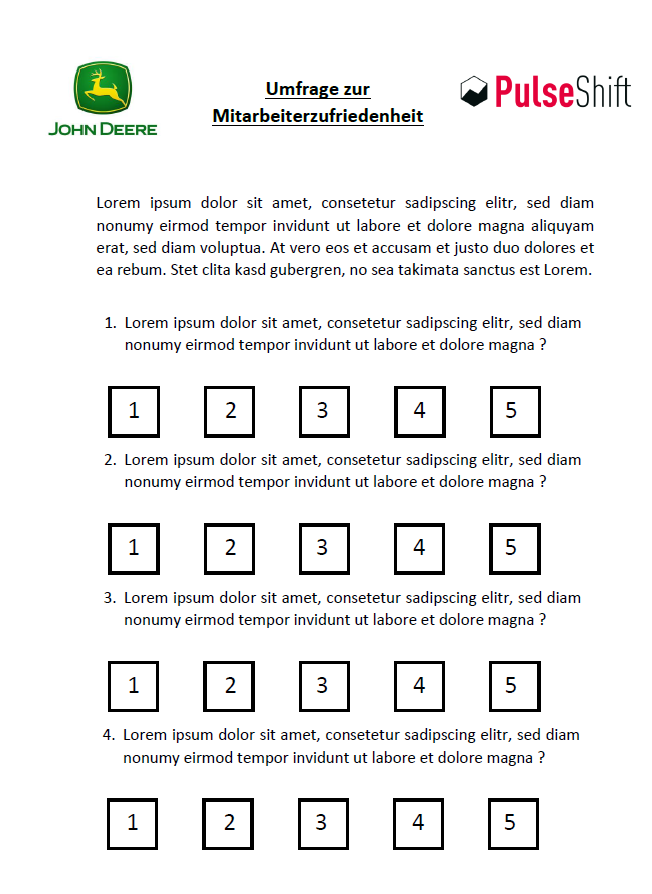
\includegraphics[width=0.9\textwidth]{images/portfolio/paper_survey}
\caption[Mockup Zettelumfrage]{Mockup Zettelumfrage}
\label{fig:portfolio:paper_survey}
\end{figure}

\subsection{Kostenfaktoren}

\begin{itemize}
\item Papier (z.B. Amazon Versando:	6 € / 500 Stück)
\item Tinte (z.B. Catridge Duck Black: 50 € / 500 Stück)
\end{itemize}

Hierbei handelt es sich nur um die Materialkosten für die gedruckten Zettel. Zusätzlich zu beachten sind die Kosten, die bei der Auswertung der Zettel anfallen. Solche sind beispielsweise Kosten zur Erstellung einer Auswertungs-Software oder Kosten für die manuelle Bearbeitung der Zettel. Diese sind aber sehr schwer zu kalkulieren und werden daher vorerst nicht geschätzt.

\subsection{Beurteilung des Projektteams}
\subsubsection{Vorteile}

\begin{itemize}
\item Keine IT-Implementierung seitens des Unternehmens benötigt
\item Schnelle und einfache Beantwortung der Zettel durch Mitarbeiter
\item Geringe Kosten und einfacher Prozess für die Erstellung der Zettel
\item Kein Authentisierungsprozess benötigt
\end{itemize}

\subsubsection{Nachteile}

\begin{itemize}
\item Aufwändiger Auswertungsprozess
\item Hohe Kosten bei der Auswertung der Zettel
\item Zielgruppen müssen lokal von anderen Gruppen trennbar sein $\rightarrow$ Wo werden die Zettel ausgelegt?
\item Zettel müssen gedruckt werden
\item Die entsprechenden Fragen müssen händisch in ein Dokument eingetragen werden
\end{itemize}

\subsubsection{Bewertung und Potential}
Für die Mitarbeiter ist die Umfrage schnell und einfach durchzuführen. Es müssen keine weiteren Applikationen installiert oder sonstige technische Voraussetzungen geschaffen werden. Allerdings erfordert die Umfrage einen hohen Arbeitsaufwand in der Vorbereitung und Auswertung. Die geringen Kosten für die Zettel selbst sind jedoch zu vernachlässigen. Insbesondere durch den Medienbruch in der Auswertung und durch den fehlenden Anreiz für die Mitarbeiter stellen die Zettel keinen geeigneten Umfragekanal dar.

\subsection{Feedback und Beurteilung durch PulseShift}

PulseShift sieht die Umsetzung einer Zettelumfrage nicht als sinnvoll an, da der Aufwand zur Auswertung der Zettel zu hoch ist. Außerdem wird der Kanal Zettelumfrage nicht als innovativ genug betrachtet, um sich von Wettbewerbern abzugrenzen.

\subsection{Weiteres Vorgehen}

Der Kanal Zettelumfrage wird sowohl vom Projektteam als auch von PulseShift kritisch betrachtet. Er wird nicht weiter verfolgt.

\section{Tablets}
\label{section:tablets}
\section{Lunchapp - Proof of Concept}
\label{section:realisation:lunchapp}

\subsection{Beschreibung}

- Was ist die Idee

- Warum Lunch und nicht z.B. Dienstplan

\subsection{Lastenheft}

\begin{itemize}
\item Es ist eine mobile Anwendung zu erstellen, die das Lunchmenü für die nächsten 5 Tage anzeigt. Dies beinhaltet den Namen, den Preis sowie die Allergene und Zusatzstoffe der einzelnen Menüs.
\item Zusätzlich sollen die Öffnungszeiten der Kantine angezeigt werden. 
\item Außerdem soll es möglich sein zwischen verschiedenen Kantinen zu wählen
\item Wenn die Kantine geschlossen ist, soll diese Information anstelle der Öffnungszeiten und des Lunchmenüs angezeigt werden.
\item Außerdem soll die Umfragefunktionalität von PulseShift direkt innerhalb der Anwendung zur Verfügung stehen und kein Absprung nötig sein.
\item In der Anwendung sollen Banner angezeigt werden können, die den Nutzer zum Teilen der App oder der Teilnahme an einer Umfrage bewegen. Diese sollen in für den Nutzer als zufällig empfundenen Zeitabständen angezeigt werden.
\item Für die Umfragefunktionalität soll der Benutzer mindestens auf eine Gruppe von Personen eingegrenzt werden können.
\item Der Nutzer soll von der Anwendung aktiv über die Möglichkeit zur Umfrage sowie Essensangebote informiert werden.
\item Das Design der Anwendung soll sich an den von PulseShift entwickelten und bereitgestellten Mockups orientieren.
\end{itemize}

\subsection{Pflichtenheft}

\begin{itemize}
\item Es wird eine \gls{pwa} erstellt, die auf verschiedenen Plattformen lauffähig ist. 
\item Diese ermöglicht das Anzeigen des Lunchs für die nächsten 5 Tage mit dem Namen, dem Preis sowie den Allergenen und Zusatzstoffen der einzelnen Menüs. 
\item Außerdem werden die Öffnungszeiten sowie eine mögliche Schließung der Kantine angezeigt.
\item Die Daten zum Lunchmenü und den Öffnungszeiten werden lokal und hart kodiert in einer JSON Datei gemockt. Eine Anbindung an einen Datenserver erfolgt nicht. 
\item Die Umfragefunktionalität die von PulseShift entwickelt wurde, wird in die Anwendung hineingerendert werden. Das Anzeigen der Umfrage wird nicht selbst implementiert. 
\item Der Server für die Umfragefunktionalität wird austauschbar sein. Damit ist gemeint, dass die URL beliebig definierbar ist.
\item Die Benutzereingrenzung wird nach einer Absprache mit PulseShift über die konkrete gewünschte Ausprägung implementiert.
\item Die Detailansicht der Lunchmenüs soll dynamisch in die View der Übersicht der Lunchmenüs integriert werden.
\item Es wird eine Bannerfunktionalität bereitgestellt, die dynamisch ausgelöst werden soll. Diese weißt den Nutzer auf das Teilen der Anwendung sowie die Möglichkeit zur Umfrage hin.
\item Für Android Geräte werden Pushbenachrichtigungen implementiert. Für iOS ist dies aufgrund der Realisierung als \gls{pwa} nicht möglich.
\item Die Anwendung soll lokal gecached werden, damit sie auch ohne Internetverbindung genutzt werden kann.
\end{itemize}

\subsection{EPK: Ablauf der Anwendung}

\subsection{Architektur}
\section{Captive Portal - Proof of Concept}
\label{section:realisation:captive_portal}
\subsection{Lastenheft}
Nach dem Treffen mit PulseShift am 08.03.2018 wurde ein Lastenheft mit den folgenden Punkten ausgearbeitet:
\begin{itemize}
\item Es soll ein Captive Portal innerhalb eines WLAN Netzwerks eingerichtet werden, das die Nutzer optional zu einer Umfrage weiterleiten kann.
\item Es sollen mehrere Hardwarelösungen mit Captive Portal Funktionalität, wie ein Raspberry Pi, ein Router oder ein Accesspoint, untersucht werden. 
\item Dabei sollen Hersteller-agnostische Lösungen gefunden werden.
\item Anschließend soll das Captive Portal durch genau eine der untersuchten Hardwarelösungen realisiert werden.
\item Die dabei benötigte Hardware soll unter Absprache mit Pulseshift von Pulseshift organisiert werden.
\item Der Nutzer, der ein Endgerät mit dem erzeugten WLAN Netzwerk verbindet, soll über die Möglichkeit zur Teilnahme an einer Umfrage informiert, jedoch nicht gezwungen werden.
\item Durch einen Redirect soll der Nutzer direkt zu einer Umfrageseite gelangen, die die Fragebögen von Pulseshift beinhaltet.
\item Die Fragebögen von Pulseshift sollen entweder lokal auf der Hardwarelösung gespeichert sein oder über das Internet direkt angesteuert werden.
\end{itemize}

\subsection{Pflichtenheft}
Anhand des zuvor erarbeiteten Lastenhefts wurde anschließend ein Pflichtenheft mit folgendem Inhalt erstellt:
\begin{itemize}
\item Es werden Hardwarelösungen mit Captive Portal Funktionalität untersucht.
\item Dabei werden Router, Accesspoints und Rasbperry Pis genauer behandelt.
\item Die Anwendungsmöglichkeiten, Vor- \& Nachteile der einzelnen Komponenten wird erarbeitet.
\item Als weiteres Auswahlkriterium wird überprüft, ob eine entsprechende Lösung unabhängig vom Hersteller der Hardware erfolgen kann.
\item Unter Absprache mit Pulseshift wird eine entsprechende Hardwarelösung von Pulseshift bereitgestellt.
\item Die gegebene Hardwarelösung wird ein WLAN Netzwerk erzeugen, indem sich Nutzer, die sich in unmittelbarer Nähe befinden, mit ihren Endgeräten anmelden können.
\item Ein Nutzer, der in diesem Netzwerk angemeldet ist, wird über die freiwillige Teilnahmemöglichkeit an einer Umfrage von Pulseshift informiert.
\item Diese Information wird in Form eines Popups auf dem entsprechenden Endgerät erscheinen.
\item Das Popup wird zwei Optionen beinhalten, die Option zur Umfrage zu gelangen und die Option nicht an der Umfrage teilzunehmen.
\item Erstere Option wird entweder per Internet direkt zu der von Pulseshift gehosteten Umfrage führen oder eine auf der Hardwarelösung lokal gespeicherte Kopie der Fragebögen anzeigen.
\item Insofern die Umfrage lokal gespeichert ist und kein Internetzugang vorhanden ist, werden die angegebenen Antworten und Informationen des Nutzers ebenfalls lokal gespeichert.
\item Die zweite Option wird das Popup schließen.
\end{itemize}



\subsection{EPK: Ablauf der Anwendung}

Die in \ref{fig:captive_epk1} dargestellte EPK zeigt den Ablauf der Captive Portal Funktionalität ohne Internet, wie er etwa bei Gesamtveranstaltungen genutzt werden kann. Nach der Verbindung des Nutzers mit dem WLAN erscheint automatisch ein Pop-up mit der Umfrageseite. Vorteil hierbei ist, dass keine URL eingegeben werden muss und die Endgeräte keinen Internetzugang benötigen. Theoretisch kann diese Lösung auch dauerhaft in der Kantine aufgestellt werden, da jedoch kein Internetzugang besteht, ist der Anreiz gering, sich mit dem WLAN zu verbinden.
\newline
\begin{figure}[H]
\centering
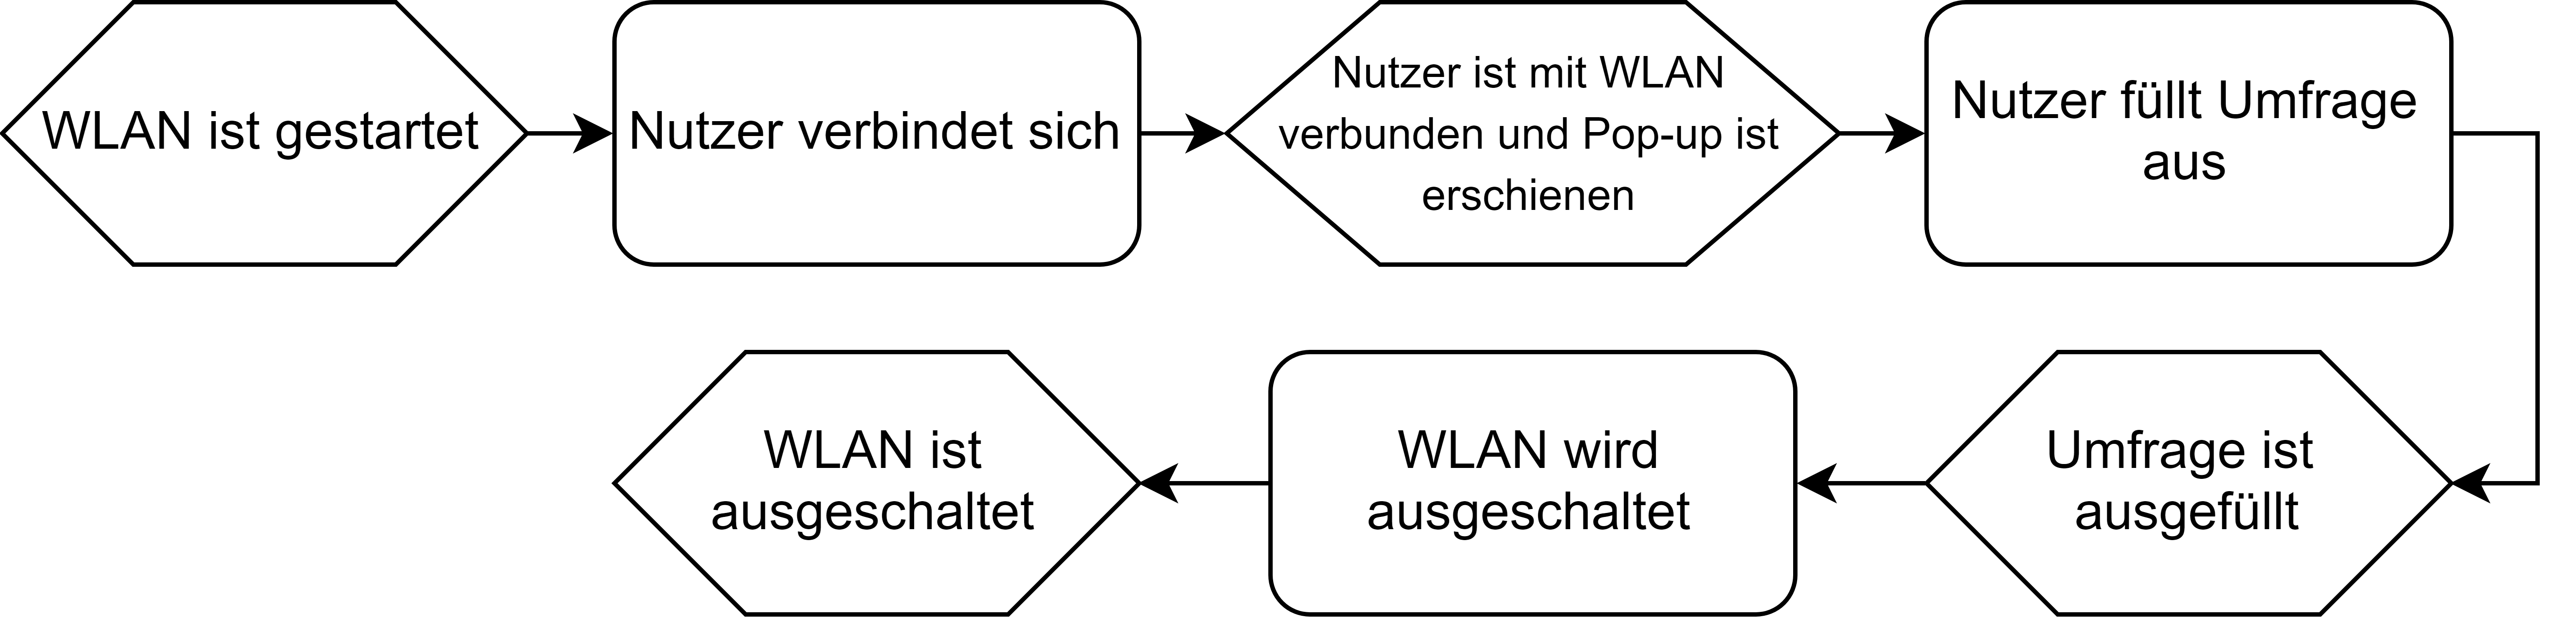
\includegraphics[width=0.9\textwidth]{images/captiveportal_EPK1}
\caption[EPK zum Ablauf ohne Internetzugang]{EPK zum Ablauf ohne Internetzugang}
\label{fig:captive_epk1}
\end{figure}


Die in \ref{fig:captive_epk2} dargestellte EPK zeigt die Verwendung eines Captive Portals mit Internetzugang. Diese Lösung könnte bei einem längerfristigen Einsatz Anwendung finden und während des Umfragezeitraums etwa in der Kantine vor den Internetzugang geschaltet werden. Nachdem sich der Nutzer mit dem WLAN verbunden hat, erscheint auch hier der Pop-up mit der Umfrageseite. Da der Nutzer nicht gezwungen werden darf, diese auszufüllen, kann sie durch einen \textit{Überspringen}-Button übersprungen werden und der Nutzer gelangt direkt ins Internet. Alternativ füllt der Nutzer die Umfrage aus und erhält im Anschluss den Zugang ins Internet. Soll die Umfrage erneut durchgeführt werden, kann der Nutzer - etwa durch einen Timeout - vom WLAN abgemeldet werden und er erhält bei der nächsten Verbindung erneut das Pop-up mit der Umfrageseite und anderen Fragen.

\begin{figure}[H]
\centering
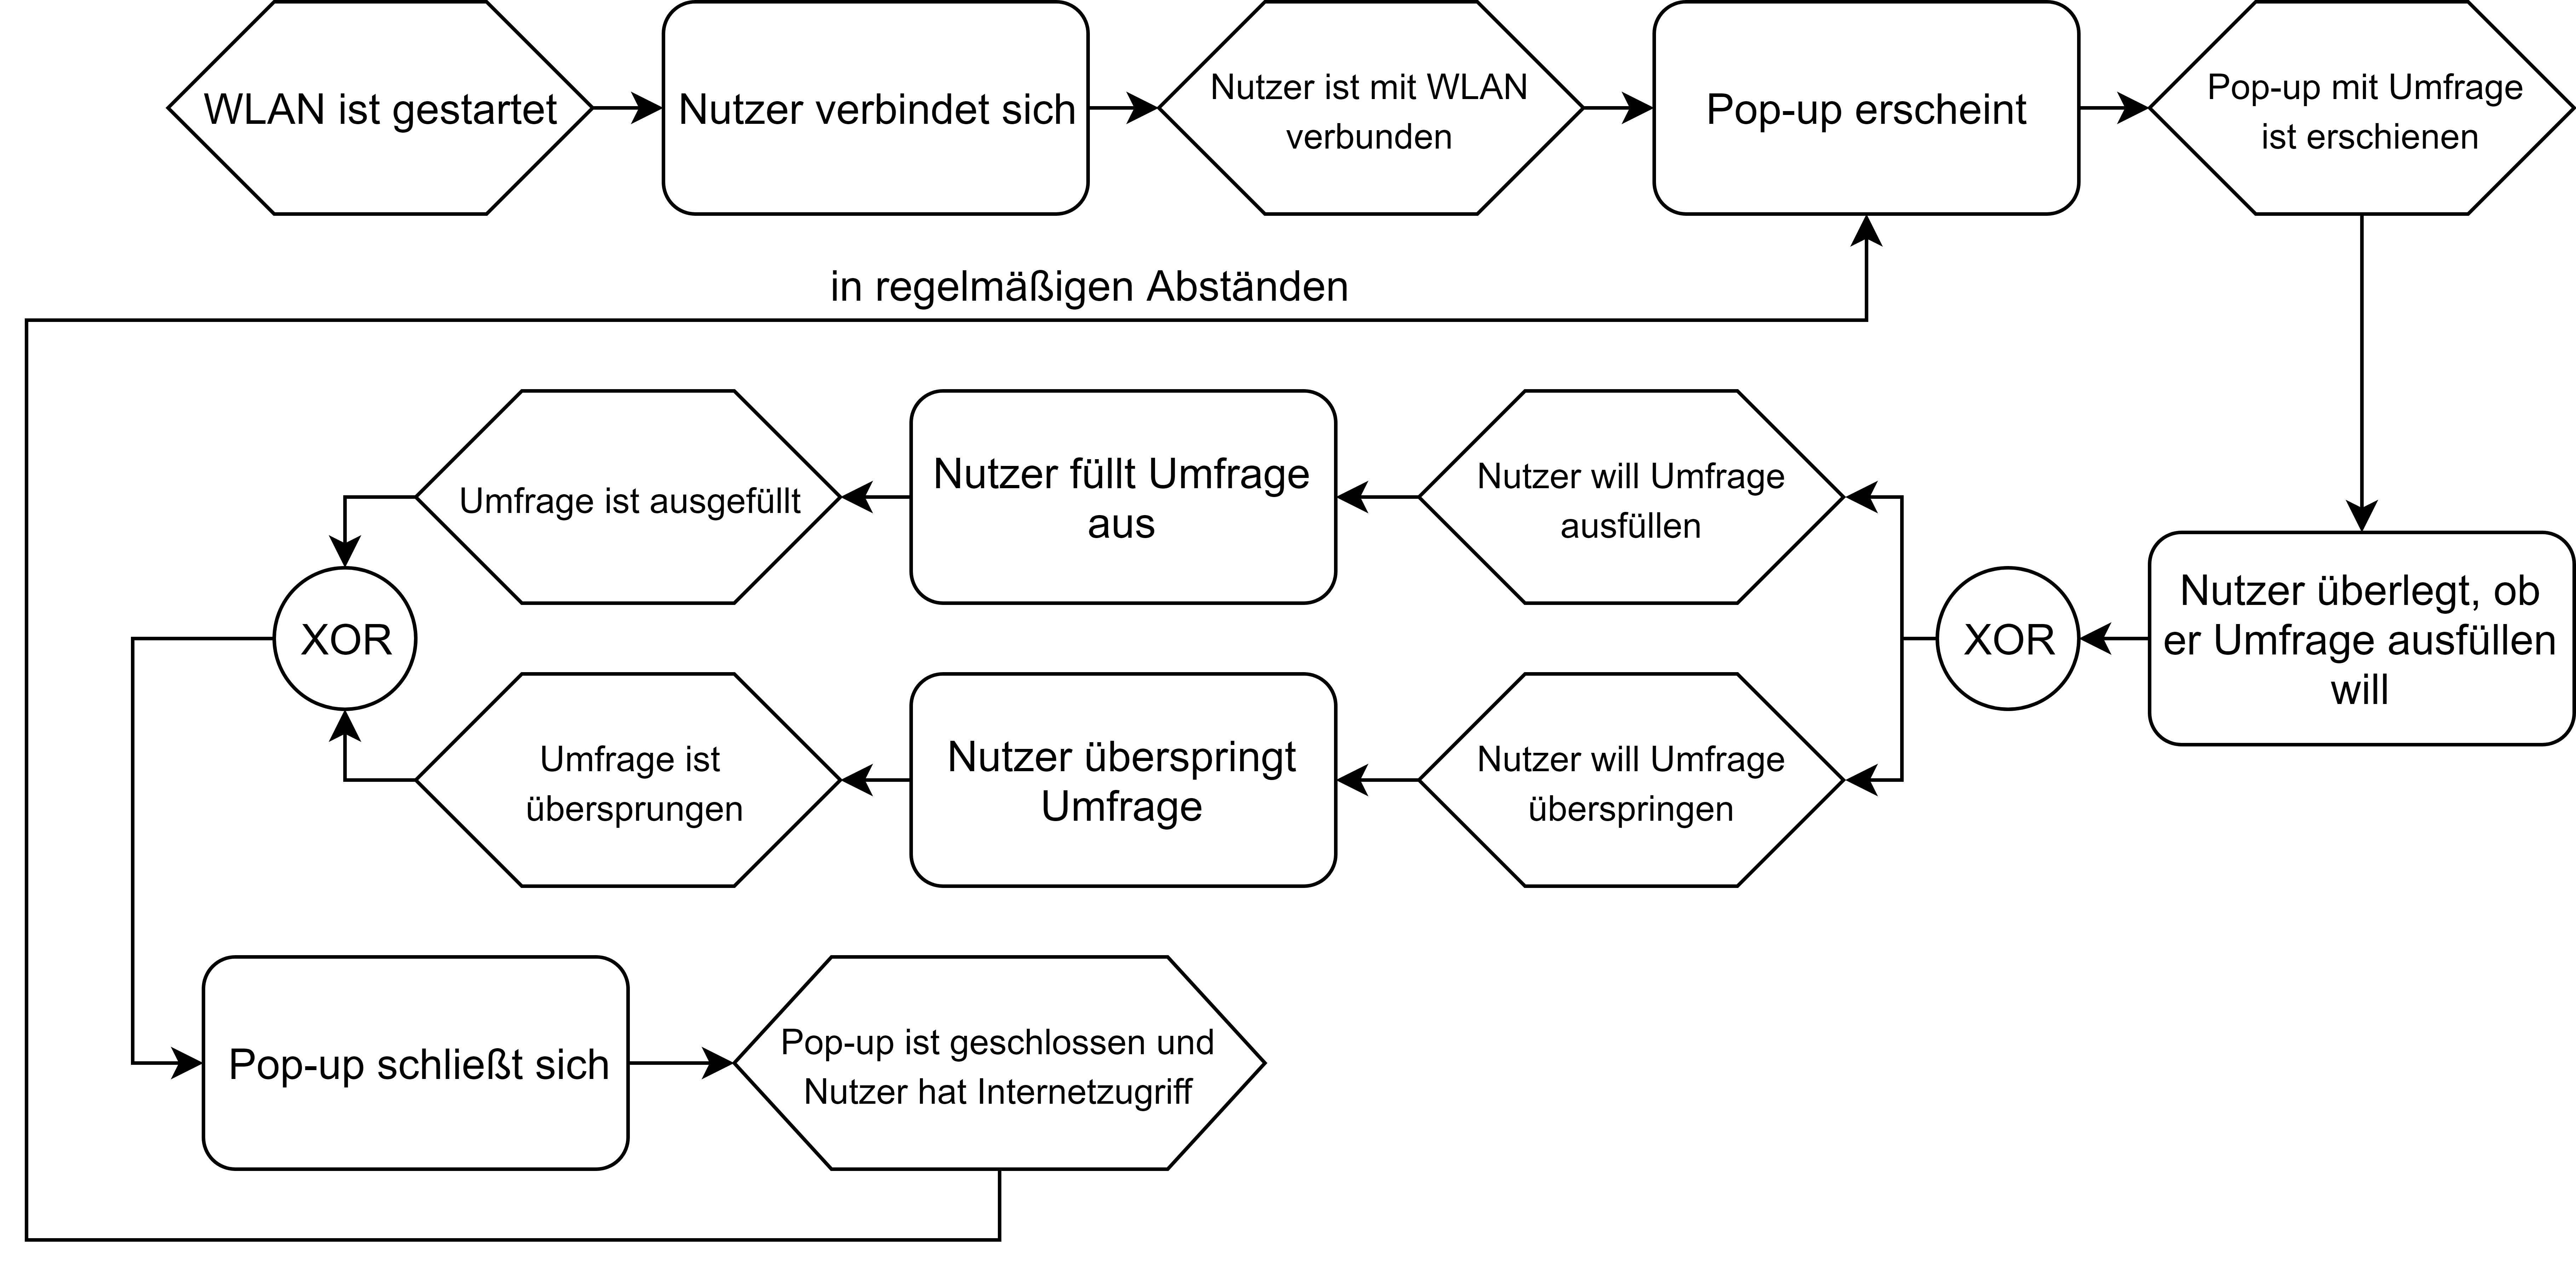
\includegraphics[width=0.9\textwidth]{images/captiveportal_EPK2}
\caption[EPK zum Ablauf mit Internetzugang]{EPK zum Ablauf mit Internetzugang}
\label{fig:captive_epk2}
\end{figure}

 
\subsection{Architektur}
\subsubsection{Verwendung eines Raspberry Pi}
\subsubsection*{Initiale Einrichtung und verwendete Hardware}
Der Raspberry Pi soll die Funktionalität eines Captive Portals für Umfragen veranschaulichen. Grundsätzlich benötigt wird hierfür:
\begin{itemize}
\item Raspberry Pi 3
\item Stromkabel
\item SD Karte
\end{itemize}

Da der Raspberry Pi 3 bereits einen WLAN-Empfänger eingebaut hat, wird kein zusätzlicher WLAN-USB-Empfänger benötigt. Zunächst muss das Betriebssystem Raspbian Stretch auf dem Raspberry Pi  installiert werden. Hierfür kann beispielsweise das Installationsprogramm \textit{NOOBS} genutzt werden, das über einen Computer auf die SD Karte gespielt wird. Anschließend erfolgt die Installation und die Aktualisierung des Betriebssystems durch \textit{apt-get update} und \textit{apt-get upgrade}.

\subsubsection*{Anleitung 1 - Captive Portal ohne Internet}
Um das Captive Portal einzurichten, wird zunächst der Ansatz ohne Internetverbindung, also mit einer lokal gehosteten Webseite, gewählt. Diese eignet sich insbesondere für die Verwendung bei Gesamtveranstaltungen, bei denen die Umfrage einmalig durchgeführt wird. Hierfür wird der unter \textit{https://brennanhm.ca/knowledgebase/2016 /10/raspberry-pi-access-point-and-captive-portal-without-internet/} zu findenden Anleitung gefolgt. Um diese umzusetzen, müssen auf dem Raspberry Pi die Pakete \textit{hostapd} und \textit{dnsmasq} installiert werden.

Das Paket \textit{hostapd} ermöglicht es, dass der WLAN-Empfänger als Access Point dienen kann, also Verbindungen von anderen Endgeräten annimmt. Bei dem Paket \textit{dnsmasq} handelt es sich um einen einfach zu konfigurierenden DNS- und DHCP-Server. Für beide Pakete müssen anschließend weitere Konfigurationen durchgeführt werden.

Das letzte Paket \textit{nginx} bietet einen Webserver, der für das lokale Hosting der Umfrage-Seite genutzt wird. Die in der Anleitung vorgeschlagene \textit{nginx}-Konfiguration wird um das rewrite-Statement für den /feedback/ Pfad ergänzt. In dem Block für den /generate\_204 Pfad können URL-Parameter mitzurückgegeben werden. Diese werden auch auf Android und auf Windows Endgeräten genutzt, bei iOS hingegen funktioniert dies nicht. Aus diesem Grund wurden diese URL-Parameter, nach unterschiedlichen Versuchen, nginx richtig zu konfigurieren, direkt in der JavaScript-Datei der Umfrage-Webseite festgelegt. Der Nutzer wird ebenfalls auf die Umfrageseite weitergeleitet, wenn er eine beliebige URL in seinen Browser eingibt.

Das Captive Portal des Raspberry Pi funktioniert mit dieser Anleitung problemlos auf Windows-Computern, iOS-Endgeräten und den meisten Android-Engeräten. Lediglich bei Samsung-Smartphones öffnet sich der Pop-up zum Anmelden am WLAN nicht. Der Grund hierfür ist nicht klar, könnte jedoch möglicherweise durch eine andere dnsmasq- oder nginx-Konfiguration behoben werden.

Die automatische Einrichtung des Raspberry Pi wird durch ein selbst erstellten Shell Skript ermöglicht, dass die Schritte in der Anleitung hintereinander durchführt. Voraussetzung ist ein neu aufgesetzter Raspberry Pi 3 mit WLAN-Interface wlan0. Der Name des WLAN-Netzwerks wird als Argument \textit{sudo bash setup.sh Name\_des\_WLANs} übergeben, die Webseite muss anschließend in den Ordner /usr/share/nginx/html/host kopiert werden.

\subsubsection*{Anleitung 2 - Captive Portal mit Internet}
Eine zweite Anleitung ermöglicht es, den Raspberry Pi als WLAN-Access Point mit Captive Portal für einen Internetzugang zu nutzen, was für den längerfristigen Einsatz - etwa in einer Kantine - geeignet wäre. Hierfür werden die Anleitungen 2a unter \textit{https://pimylifeup.com/raspberry-pi-wireless-access-point/} für die Einrichtung des Access Points und 2b unter \textit{https://pimylifeup.com/raspberry-pi-captive-portal/} für die Captive Portal Funktionalität genutzt.

Für die Einrichtung des Access Points werden erneut die Pakete \textit{hostapd} und \textit{dnsmasq} genutzt. Zusätzlich werden die IP-Tabellen verändert und diese Veränderungen und ein Neustart von \textit{hostapd} und \textit{dnsmasq} in die rc.local Datei geschrieben, damit diese bei jedem Neustart umgesetzt werden. Dies hat jedoch bei dem Austesten der Anleitung nicht funktioniert, sodass ein \textit{sleep 10} Befehl der rc.local Datei hinzugefügt werden musste.

Im zweiten Schritt wird für den Access Point die Captive Portal Funktionalität hinzugefügt. Hierfür wird die Software \textit{nodogsplash} auf dem Raspberry Pi installiert. Diese hostet lokal die Captive Portal Seite in dem Verzeichnis \textit{/etc/nodogsplash/htdocs/splash.html}. Auf der Captive Portal Seite kann ein Formular abgeschickt werden, mit dem der Nutzer authentifiziert wird und mit dem er Zugriff auf das Internet erhält. Dieses kann zum Überspringen der Umfrage direkt oder erst nach dem Ausfüllen der Anfrage abgeschickt werden. Hierfür müsste der Umfrage-Webapp ein \textit{Überspringen}-Button und ein \textit{Umfrage abschließen}-Button hinzugefügt werden, durch die das Formular abgeschickt wird. In der nodogsplash.conf Datei können weitere Konfigurationen vorgenommen werden, insbesondere auch der Internetzugriff für nicht-authentifizierte Nutzer erlaubt werden, sodass auf der Captive Portal Seite Inhalte aus dem Internet angezeigt werden.

Diese Lösung funktioniert auf allen Endgeräten, insbesondere auch auf denen von Samsung. Liegt kein Internet vor, funktioniert das Captive Portal jedoch nicht. Hierfür muss in der dnsmasq.conf Konfigurationsdatei \textit{address=/\#/IP\_des\_Raspberry} zur Auflösung aller Domainnamen auf den Raspberry Pi hinzugefügt werden. Ist dies erfolgt, funktioniert das automatische Pop-up bei Samsung Smartphones jedoch nicht mehr.

Auch für diese Anleitungen wurden Shell Skripte umgesetzt. Diese können mit \textit{sudo bash setup2a.sh Name\_des\_WLANs Passwort\_des\_WLANs} und \textit{sudo bash setup2b.sh} ausgeführt werden.

\subsubsection*{Weiteres Vorgehen}
Die Umsetzung des Captive Portals mithilfe des Raspberry Pi dient in erster Linie zur Veranschaulichung der Möglichkeit, die Umfrage in dieser Form umzusetzen. Sollte eine der Lösungen des Raspberry Pi tatsächlich in einem produktiven Umfeld genutzt werden, sind folgende Aspekte zu beachten:
\begin{itemize}
\item Es sollte ein externer WLAN-Empfänger genutzt werden, da der in dem Raspberry Pi eingebaute Empfänger vermutlich eine zu geringe Signalstärke hat. In diesem Fall müssten die Konfigurationen entsprechend angepasst werden. Gleichzeitig muss überprüft werden, wie viel Verbindungen gleichzeitig unterstützt werden können.
\item Das Problem der automatischen Pop-ups bei Samsung Handys muss behoben werden, das Problem liegt womöglich an der DNS-Auflösung oder der zurückgegebenen Status-Codes.
\item Die Anleitungen müssen vertieft auf die Aspekte Sicherheit und Performance überprüft werden, möglicherweise auch eine SSL-Verschlüsselung eingerichtet werden. Die Lösungen sollten in der bestehenden Form noch nicht produktiv genutzt werden, da Sicherheitsrisiken bestehen, die insbesondere bei der zweiten, längerfristigen Lösung mit Internetzugang gefährlich sind.

\end{itemize}

\subsubsection{Alternative Ansätze}
Neben der Verwendung des Raspberry Pi gibt es verschiedene Hardware- und Softwarelösungen, die ebenfalls die Captive Portal Funktionalität bieten. Vorteil von diesen ist, dass es sich in der Regel bereits um fertig konfigurierte und funktionierende Lösungen handelt; Nachteil ist hingegen, dass häufig wenig Konfigurationen möglich sind.

Bietet ein Unternehmen seinen Mitarbeitern einen WLAN-Internetzugang an, so wird dieser meist über zentral verwaltete Access Points realisiert. Hier besteht die Möglichkeit, dass der Access Point bereits eine Captive Portal Funktionalität besitzt. Die meiste vorinstallierte Software besitzt jedoch nur die Möglichkeit, eine einfache Webseite zum Akzeptieren der Nutzungsbedingungen anzuzeigen, sodass die eigene Umfrageseite nicht einfach eingebunden werden kann (z.B. nur als Redirect nach dem Akzeptieren der Nutzungsbedingungen). Aus diesem Grund ist es unwahrscheinlich, dass die Umfrageseite als Captive Portal direkt in der Access Point Software eines Unternehmens aktiviert werden kann.

Eine andere Lösung ist es, beispielsweise die Firewall- und Router-Software pfSense vor die Access Points oder bei Gesamtveranstaltungen vor einen eigenen Access Point zu schalten. Diese ermöglicht ebenfalls die Captive Portal-Funktionalität. Der Einsatz ist jedoch in einem Firmennetzwerk er unwahrscheinlich, da ein größerer Eingriff in die Ntzwerkinfrastruktur erforderlich ist.

Als Alternative könnte auch das Betriebssystem eines kompatiblen Routers durch das auf Linux basierende, weit verbreitete Betriebssystem OpenWRT überschrieben werden, um diesen selbst zu konfigurieren. In diesem Fall ähneln die Konfigurationsarbeiten denen auf dem Raspberry Pi und für die Captive Portal Funktionalität kann eine Software wie nodogsplash, Wifidog oder CoovaChilli genutzt werden.




\subsubsection{Anforderungserfüllung}
Die zentralen Anforderungen des Lasten- und Pflichtenhefts wurden erfüllt. Mit der ausgewählten Hardware - einem Raspberry Pi - wurde das Captive Portal prototypisch eingerichtet. Die verwendeten Lösungsansätze können somit als Demo, für praktische Tests (zur Einschätzung, ob dieser Umfragekanal geeignet ist) und als Grundlage für eine spätere produktive Nutzung dienen. Zudem wurden mögliche Probleme, wie etwa die Verwendung von Samsung Endgeräten, aufgedeckt.

Weniger intensiv wurden hingegen die alternativen Lösungsansätze betrachtet, da diese sehr Hardware-abhängig sind und diese Hardware für eine sinnvolle Einschätzung durch Austesten nicht zur Verfügung stand. Aus diesem Grund wurden diese nur konzeptionell beschrieben.


\section{Newsfeed App - Recherchebericht}
\label{section:realisation:newsfeed_app}


Newsfeed App for deskless/frontline employees Firstline workers
\begin{itemize}
\item {Mircosoft Staffhub https://products.office.com/de-de/microsoft-staffhub/staff-scheduling-software}
\item {Inkling 	https://www.inkling.com/ }
\item {Zinc https://www.zinc.it/ Beliebteste/Am häufigsten genutzte App für „Deskless“ Mitarbeiter}
\item {Slack https://slack.com/intl/de-de Desktop worker or/and Frontline worker?}
\item {Nicht geeignet: Whatsapp Business https://www.deutsche-handwerks-zeitung.de/whatsapp-betrieblich-nutzen-was-beim-datenschutz-wirklich-gilt/150/3101/363865}
\end{itemize}


\subsection{Lastenheft}
\begin{itemize}
\item Es ist ein Recherchebericht zu erstellen, der sich mit Produkten, Lösungen und Anwendungen (im Folgenden als Anwendungen zusammengefasst) befasst. Konkret geht es um Anwendungen, die es Unternehmen ermöglichen, ihre Mitarbeiter über unternehmensinterne Vorgänge zu informieren und den Mitarbeitern eine Interaktion mit dem Unternehmen ermöglichen. 
\item Der Bericht soll eine Übersicht über die am Markt etablierten Anwendungen liefern. Ein Fokus soll auf den Anreizen liegen, mit welchen die Anwendungen die Mitarbeiter zur Benutzung motivieren.
\item Des Weiteren soll im Bericht untersucht werden, welche Umfragefunktionalitäten in der jeweiligen Anwendung bereits existieren und wie diese potentiell durch PulseShift genutzt werden könnten. 
\item Darüber hinaus soll der Bericht aufzeigen, welche weiteren Möglichkeiten zur Einbindung einer Umfrage durch PulseShift es jeweils gibt und wie flexibel diese Möglichkeiten genutzt werden können.
\item Außerdem sollen in dem Bericht die Erfahrungen von Referenzkunden, die die Anwendung bei Offline-Mitarbeitern einsetzen, beschrieben werden. 
\item Sofern jeweils eine Preisstruktur verfügbar ist, soll außerdem auf diese eingegangen werden.
\end{itemize}

\subsection{Pflichtenheft}
\begin{itemize}
\item Es wird ein Recherchebericht erstellt, der sich mit Produkten, Lösungen und Anwendungen (im Folgenden als Anwendungen zusammengefasst) befasst. Konkret wird es um Anwendungen gehen, die es Unternehmen ermöglichen, ihre Mitarbeiter über unternehmensinterne Vorgänge zu informieren und den Mitarbeitern eine Interaktion mit dem Unternehmen ermöglichen.
\item Der Bericht wird eine Übersicht über die am Markt etablierten Anwendungen liefern. Für die Marktführer wird herausgearbeitet, mit welchen Anreizen sie die Mitarbeiter zur Benutzung der Anwendung motivieren. Sofern jeweils möglich werden die Anwendungen dazu neben einer Internetrecherche auch aktiv getestet.
\item Des Weiteren werden im Bericht die Möglichkeiten zur Integration der Umfrage von PulseShift in die jeweilige Anwendung aufgezeigt. Diese wird tabellarisch mit zusätzlichen erläuternden Texten gegenübergestellt. Dabei wird sofern jeweils verfügbar sowohl auf die Umfragefunktionalitäten der Anwendung als auch das Abspringen zur Umfragefunktion von PulseShift eingegangen. Außerdem werden jeweils mögliche weitere anwendungsspezifische Möglichkeiten wie beispielsweise ein Einbinden der Umfrage mittels iFrame vorgestellt.
\item Abschließend werden die Erfahrungen von Referenzkunden dargelegt. Dabei wird der Fokus auf Erfahrungen liegen, die im unmittelbaren Zusammenhang mit dem Einsatz bei Offline-Mitarbeitern stehen.
\item Der Bericht wird innerhalb des Projektabschlussberichts in Latex erstellt.
\end{itemize}


\subsection{Firstline Worker}

Die Firstline Workforce klassifiziert alle Mitarbeiter ohne festen Computer-Arbeitsplatz. Sie repräsentieren die mehr als zwei Milliarden Menschen  in Rollen, die sie zum ersten Kontaktpunkt zwischen einem Unternehmen und der Außenwelt machen. Sie sind die Menschen hinter der Theke, am Telefon, in den Kliniken und in der Werkstatt. Sie bilden das Rückgrat vieler der weltweit größten Branchen - Einzelhandel, Restaurants, Gastgewerbe, Reisen, Fertigung und Bauwesen. In dieser Rolle sind sie oft die ersten, die Kunden ansprechen, die ersten, die die Marke eines Unternehmens repräsentieren und die ersten, die Produkte und Dienstleistungen in Aktion sehen.


\begin{figure}[H] 
\centering 
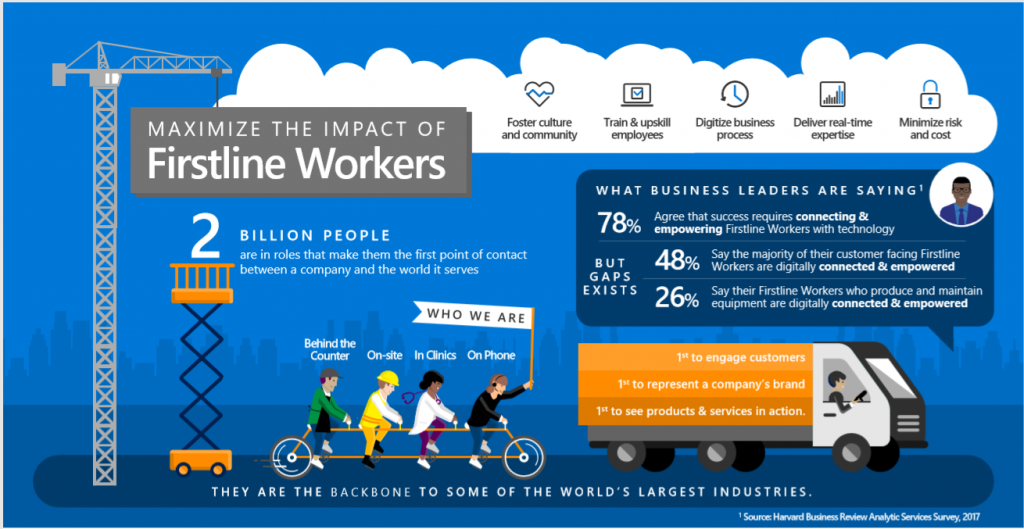
\includegraphics[scale=0.48]{images/frontlineworkers} 
\caption[Frontline Workers]{Firstline workers Aufgabenbereiche\protect} 
\label{dem} 
\end{figure}


\subsection{Microsoft Staffhub}

Microsoft StaffHub ist eine speziell für die Firstline Workforce in Office 365 entwickelte App . Es wurde speziell entwickelt, um die Fähigkeiten, Werkzeuge und Informationen zu liefern, die Firstline Mitarbeiter benötigen, um effektiv zu arbeiten und Spitzenleistungen zu erbringen. Dieser Service kombiniert Terminplanung, Aufgabenverwaltung, Dokumente, Personen und Tools an einem sicheren Ort - mit der Möglichkeit, sich mit anderen arbeitsbezogenen Apps und Ressourcen zu verbinden.
\begin{itemize}
\item Zugriff auf Schichtenplan
\item Kommunikation innerhalb des Teams
\item Zugriff auf wichtige Information übers Handy
\item Manager können Schichtenplan bearbeiten und Informationen verbreiten
\end{itemize}

\subsubsection{Verfügbarkeit}
Microsoft StaffHub ist derzeit verfügbar im Web, iOS und Android. Derzeit ist Staffhub nicht als eigenständiges Projekt sondern nur im Rahmen der folgenden Office 365-Geschäftspläne verfügbar: F 1, E1, E3 und E5. Wenn ein Kunde bereits einen dieser Pläne hat, kann er direkt Microsoft StaffHub verwenden. Der Einstieg ist ganz einfach. Erstanmelder können sich mit ihrem Office-365 Arbeitskonto unter http://staffhub.office.com anmelden. Von dort aus können sie Zeitpläne für ihre Teams erstellen und verwalten, wichtige Ressourcen und Unternehmensnachrichten hochladen und teilen und Firstline Workers einladen um die Anwendung herunterzuladen.

\subsubsection{Schedule \& Task Management}
Das Schedule \& Task Management ermöglicht es dem Manager die Schichten für die Mitarbeiter zuzuweisen, zu aktualisieren und allgemein zu verwalten. Die Mitarbeiter können gleichzeitig untereinander Schichten tauschen und Urlaub beantragen während der Manager stets die komplette Übersicht und Kontrolle bei Änderungen beibehält. 

\begin{figure}[H] 
\centering 
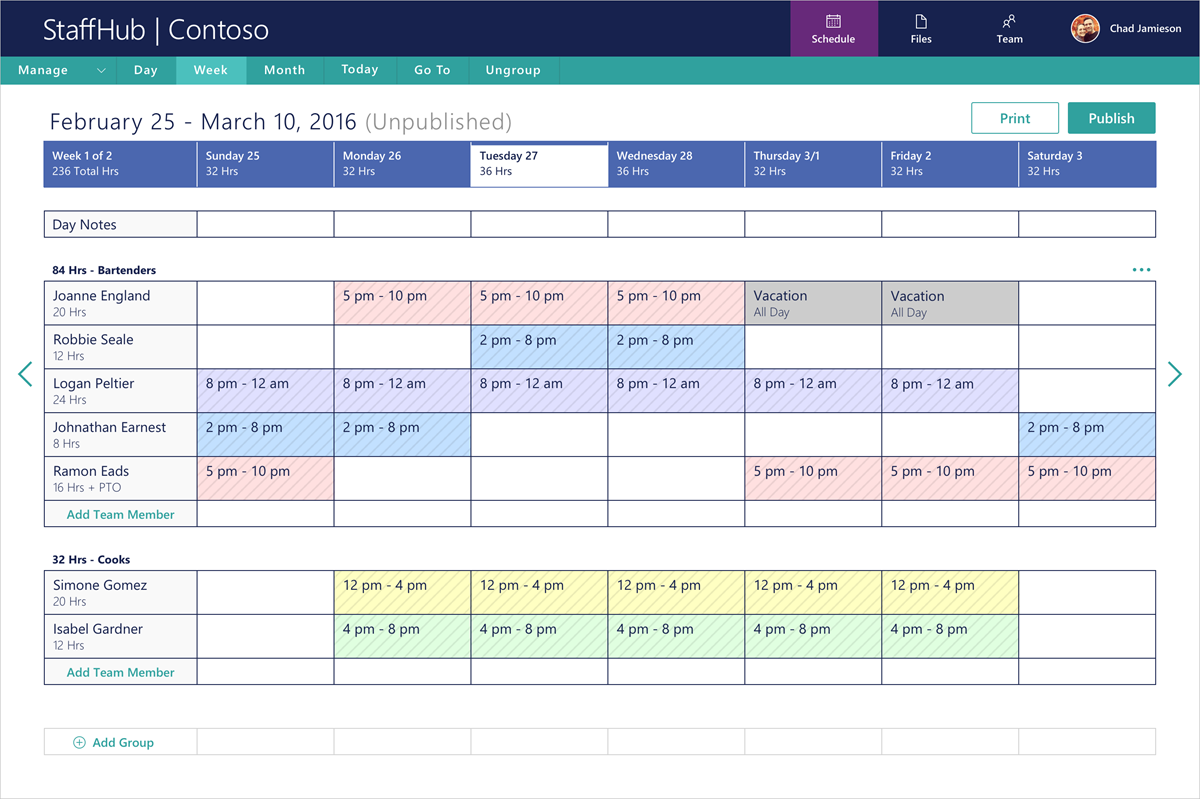
\includegraphics[scale=0.48]{images/schedule} 
\caption[Webansicht Schichtpläne]{Webansicht Schichtpläne\protect} 
\label{ws} 
\end{figure}

\begin{figure}[H] 
\centering 
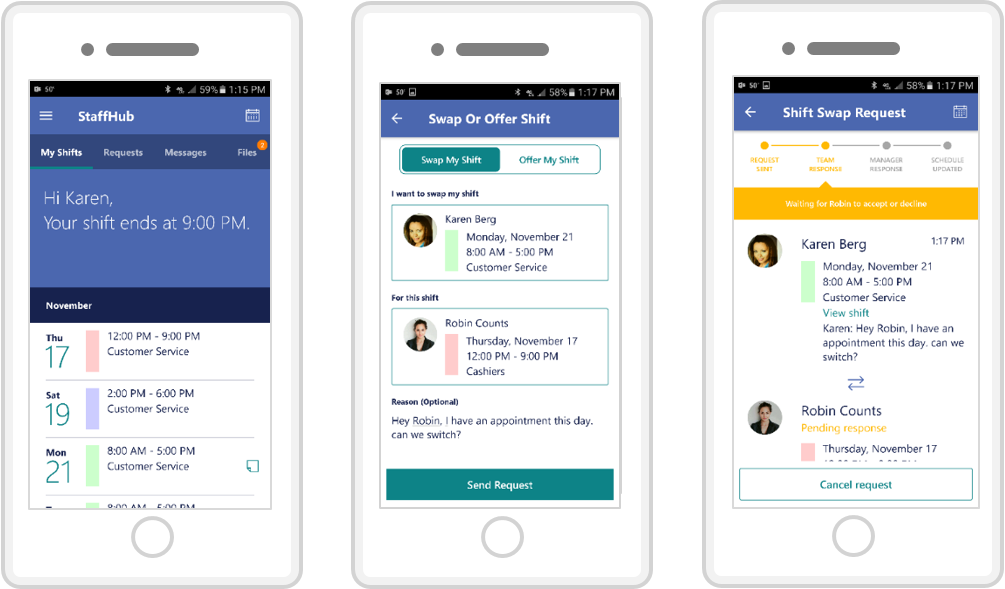
\includegraphics[scale=0.48]{images/schedulemobile} 
\caption[Schichtpläne tauschen mit dem Handy]{Schichtpläne tauschen mit dem Handy\protect} 
\label{ws} 
\end{figure}

Außerdem können einzelne Aufgaben und To-Dos vergeben werden. Diese können direkt durch den Manager vergeben werden oder der Mitarbeiter kann diese selbst als Erinnerung für sich anlegen. 

\begin{figure}[H] 
\centering 
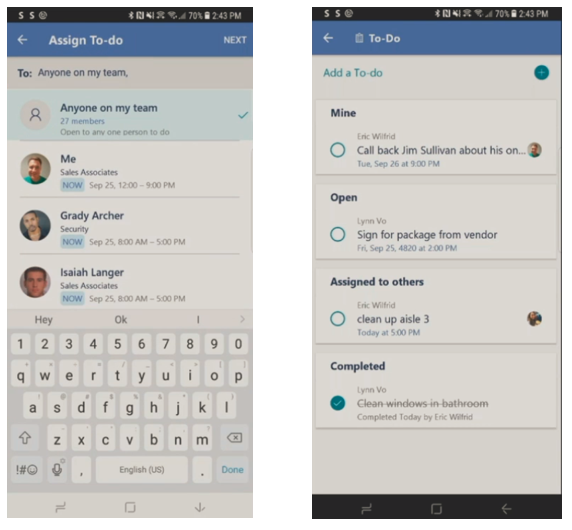
\includegraphics[scale=0.78]{images/todolist} 
\caption[To-Do Liste pflegen]{To-Do Liste pflegen\protect} 
\label{ws} 
\end{figure}

Für die Zukunft ist außerdem geplant mit Hilfe der App eine Zeiterfassung in Realtime zu ermöglichen, sodass nicht mehr klassisch gestempelt werden muss.
Zusätzlich ist es möglich die Funktionalitäten zu erweitern und weitere Services und Apps an Staffhub anzubinden. Zusätzlich ist es möglich die Funktionalitäten zu erweitern und weitere Services und Apps an Staffhub anzubinden.

\subsubsection{Communications \& Community}

In Staffhub können jederzeit neue Kommunikationskanäle aufgesetzt werden, wodurch es möglich ist Gruppen oder persönliche Chats zu starten. Des Weiteren können von dem Unternehmen direkt Best Practices oder Neuigkeiten durch Announcements an den Mitarbeiter kommuniziert werden.

\begin{figure}[H] 
\centering 
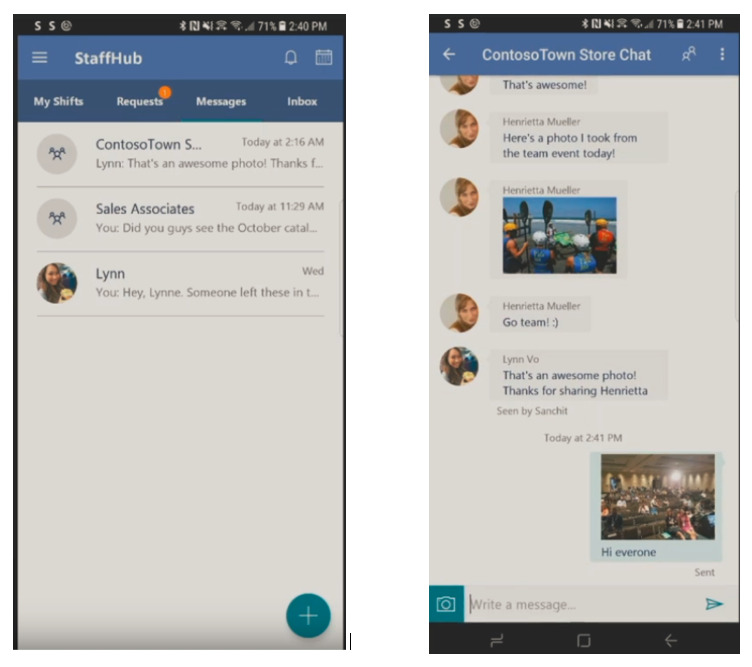
\includegraphics[scale=0.78]{images/groupchat} 
\caption[Teamchats]{Teamchats\protect} 
\label{ws} 
\end{figure}

\subsubsection{Training \& Onboarding}

Mit Staffhub ist es möglich Dokumente und Dateien zu verwalten und innerhalb des Unternehmens zu teilen. Dies wird unter anderem durch die Integration von SharePoint und team sites unterstützt. Auf den Inhalt kann man dabei direkt innerhalb der App zugreifen und dadurch Training und Oboarding Aktivitäten planen.

\begin{figure}[H] 
\centering 
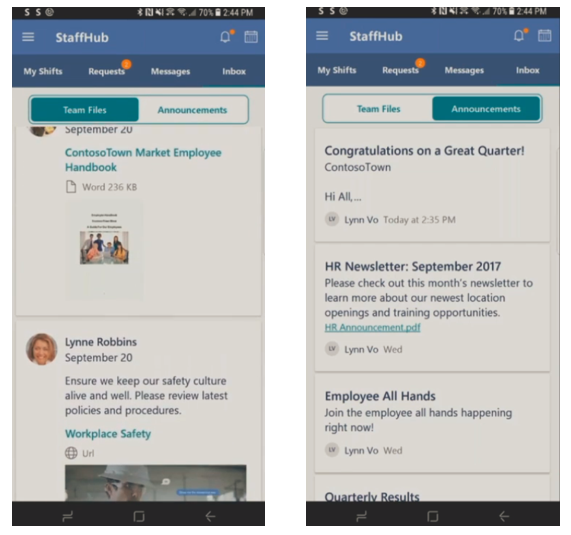
\includegraphics[scale=0.78]{images/communication} 
\caption[File Sharing und Announcements]{File Sharing und Announcements\protect} 
\label{ws} 
\end{figure}

\subsubsection{Identity \& Access Management}

Staffhub ermöglicht die Vergabe von Identitäten mit Hilfe von nur einer Telefonnummer. Eine Email-Adresse ist in diesem Fall optional. Die einzelnen User können dabei zentral mit Office 365 verwaltet werden.

\begin{figure}[H] 
\centering 
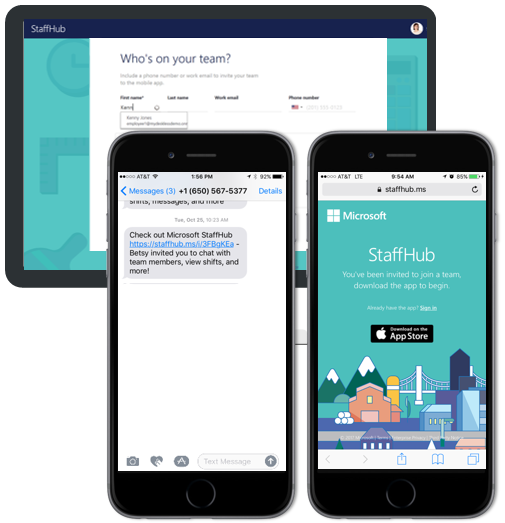
\includegraphics[scale=0.82]{images/invite} 
\caption[Telefonnummer statt E-Mail zur Identifikation]{Telefonnummer statt E-Mail zur Identifikation\protect} 
\label{ws} 
\end{figure}

\subsubsection{API \& Business Integration}

In Staffhub können über die API 3rd Party Lösungen für Workforce Management eingebunden werden. Des Weiteren kann man benutzerspezifische Integration für interne Applikationen und Prozesse hinzufügen. Zusätzlich ist die Integration mit Kronos WorkForce Central V8 unterstützt und es werden Connectors bereitgestellt um mit Microsoft Flow zu arbeiten.
Die API ist nach eigenen Angaben zunächst nur als private Vorschau verfügbar. Jedoch ist eine Erweiterung der API in naher Zukunft geplant und bei weiteren Integrationen und möglichen Partnerschaften kann man sich direkt an staffhubinfo@microsoft.com wenden. Die APIs soll nach einigen Tests und Optimierungen der Öffentlichkeit kostenlos zur Verfügung gestellt werden.

\begin{figure}[H] 
\centering 
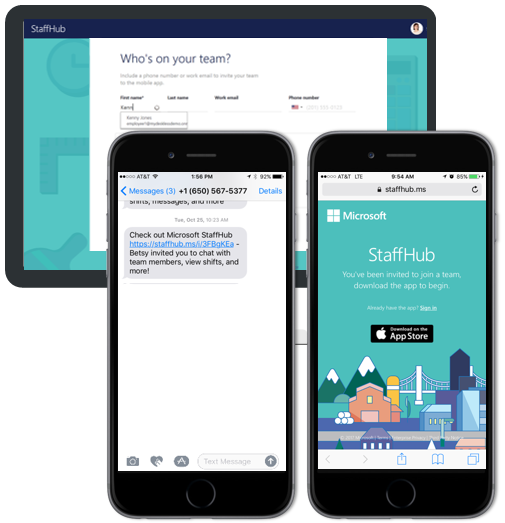
\includegraphics[scale=0.72]{images/invite} 
\caption[Cheat Sheet über Schnittstellen]{Cheat Sheet über Schnittstellen\protect} 
\label{ws} 
\end{figure}

\subsubsection{Unterschied zu Microsoft Teams}
Microsoft Teams ist ein Chat-basierter Arbeitsbereich, der Personen, Unterhaltungen und Inhalte zusammenführt. Microsoft StaffHub ist hingenen eine speziell entwickelte App für die Firstline Workforce zur Verwaltung ihres Arbeitstages. Laut Microsoft ist die Kommunikation für beide wichtig und kündigten kürzlich die Integration von StaffHub Messaging und Microsoft Teams an, um es Firstline Workers zu ermöglichen, sich mit allen Mitarbeitern zu verbinden und zusammenzuarbeiten.
 
\subsubsection{Bewertung}
Insgesamt erweist sich Microsoft Staffhub als sehr umfrangreiches und mächtiges Tool, obwohl es erst vor kurzem für die Öffentlichkeit verfügbar ist. Dadurch besteht die Möglichkeit, dass PulseShift sich die Funktionen von Staffhub zu Nutzen machen kann und die Umfrage in das Tool einzubinden. Dafür gibt es mehrere Optionen: PulseShift kann ein eigenen User beantragen und ist neben allen Mitarbeitern innerhalb des nutzenden Unternehmens zusätzlich als Drittpartei eingebunden. Dies ermöglicht dass PulseShift in einem Teamchat regelmäßig auf die Umfrage aufmerksam machen kann oder die Umfrage zentral an alle Mitarbeiter über ein Announcement verteilen, da es problemlos möglich ist ein Link oder ein Dokument innerhalb der App aufzurufen. Außerdem kann es jedem Nutzer individuell als To-Do Task assigned werden, wodurch der Mitarbeiter sich eher in der Verpflichtung sieht diese Aufgabe auch abzuhaken.
Darüber hinaus besteht mit der API, die in Zukunft weiter ausgebaut wird auch die Umfrage als Applikation von außen über eine Schnittstelle einzubinden.

\subsection{Cotap}
Cotap ist eine von Zinc entwickelte mobile Nachrichtenapplikation für das Unternehmensumfeld. Sie ist insbesondere für \glqq Deskless\grqq Unternehmen geeignet. Es soll dem Unternehmen ermöglichen schnell und einfach mit seinen Mitarbeitern zu kommunizieren. 

Die Funktionalitäten der Applikation lassen sich in zwei Hauptkategorien aufteilen. 

\begin{itemize}
\item Kommunikationstools - zur Kommunikation im Unternehmen 
\item Analysetools - zur Analyse des Kommunikationsverhalten und somit auch zur Analyse der Unternehmenssituation
\end{itemize}

Folgend werden diese Tools aufgegliedert in die einzelnen Funktionsbereiche vorgestellt.

\subsubsection{Kommunikationstools}

\begin{itemize}
\item 1:1 Messages - senden von direkten Nachrichten an jedem aus der Organisation
\item Group Messages - um sich beispielsweise innerhalb einer Abteilung abzustimmen
\item Content Sharing - um Dokumente und weitere wichtige Informationen mit anderen Mitarbeiten zu teilen
\item Hands Free - Nachrichten werden laut vorgelesen und können eingesprochen werden
\item 3RD Party Messaging - Personen, die nicht der eigenen Organisation zugeordnet sind können einfach über die E-Mail-Adresse hinzugefügt werden
\item Push to Talk - Schnelle und einfache Benachrichtigung anderer Mitarbeiter oder Gruppen durch Walkie Taklie Funktion
\item Broadcast - zum Versenden dringender und wichtiger Nachrichten an alle Beteiligten, zusätzliche Funktionalität eines Pop-Ups
\end{itemize}

Die drei letzte Komponenten 3RD Party Messaging, Push to Talk und Broadcast können für unseren Use Case genutzt werden.

3RD Party Messaging kann es PulseShift ermöglichen, über einen Gruppenchat, in welchen sie eingeladen wurden, einen Link zur Umfrage zu posten. So könnten jeweils einzelne Abteilungen gezielt erreicht werden.

Durch Push to Talk kann darauf aufmerksam gemacht werden, dass es eine Umfrage gibt an der man teilnehmen kann. Hier ist es jedoch entscheidend, dass die Übertragung der Nachricht in Tonform und live ist. 

Mit Hilfe des Broadcasts könnte ein Link zur Umfrage versendet werden. So wird dem Mitarbeiter zusätzlich suggeriert, dass es wichtig ist an dieser Umfrage teilzunehmen. 

\subsubsection{Analysetools}
Mit Hilfe der Analysetools werden die gesendeten Nachrichten, hinsichtlich Menge, Inhalt, Länge und weiteren Kriterien analysiert, um weitere Informationen zu generieren. 

Die verschiedenen Analysen werden folgend kurz dargestellt: 

\begin{itemize}
\item Analyse der einzelnen Kommunikationskanäle
\item Historischer Verlauf der Broadcasts
\item Analyse der Anzahl und Größe von gesendeten Nachrichten
\item Networkmap, um zu zeigen wer mit wem kommuniziert
\end{itemize}

Aus diesen Informationen könnte ein Mehrwert für die Umfragen geschlossen werden, dazu wäre jedoch eine komplette Erweiterung des Umfragekonzeptes notwendig und wird daher vorerst verworfen.

\subsubsection{Integrationsmöglichkeiten}
Cotap bietet die Möglichkeit andere Apps zu integrieren, sodass der Nutzer die App nicht verlassen muss, um mit anderen Apps zu interagieren. Mit Hilfe dieser Funktionalität könnten die Umfragen von PulseShift sehr einfach eingebunden werden. 

Außerdem können automatische Benachrichtigungen erstellt werden, um die Mitarbeiter auf die Umfrage hinzuweisen.

\subsubsection{Kosten}
Die App Cotap kann zunächst einmal kostenlos im Playstore herunter geladen werden. Mit Hilfe dieser kostenlosen Version können unbegrenzt Nachrichten gesendet werden, sowie Fotos, Videos und der eigene Standort geteilt werden. Außerdem sind Basic-Integrationen möglich. 

Für 5 Dollar monatlich soll es möglich sein, Audio und Video Anrufe bis zu 100 Minuten pro Nutzer pro Monat zu tätigen und Daten bis zu zwei GB pro User pro Monat zu versenden. In diesem Paket ist außerdem die Gruppenorganisation und Nutzung enthalten. Des weiteren können individuelle Benachrichtigungen erstellt werden.

Das teuerste Paket ist für 10 Dollar pro Monat zu erhalten. Hier können Audio und Video Anrufe bis zu 250 Minuten pro Nutzer pro Monat getätigt werden. Außerdem können unlimitiert Daten versendet und empfangen werden. Nun können Enterprise-files sowie ein Single Sign-One integriert werden. Außerdem wird alles aktiv überwacht und die Analysetools somit genutzt werden.

\subsubsection{Bewertung}
Cotap erscheint als eine gute Möglichkeit, um die Umfragen von PulseShift zu integrieren. Die genaue Zusammenarbeit mit Cotap, PulseShift und dem jeweiligen Unternehmen muss jedoch abgeklärt werden, sowie die genauen Kosten ermittelt werden.



\chapter{Realisierung vielversprechender Umfragekanäle}
\label{chapter:realisation}
\section{Lunchapp - Proof of Concept}
\label{section:realisation:lunchapp}

\subsection{Beschreibung}

- Was ist die Idee

- Warum Lunch und nicht z.B. Dienstplan

\subsection{Lastenheft}

\begin{itemize}
\item Es ist eine mobile Anwendung zu erstellen, die das Lunchmenü für die nächsten 5 Tage anzeigt. Dies beinhaltet den Namen, den Preis sowie die Allergene und Zusatzstoffe der einzelnen Menüs.
\item Zusätzlich sollen die Öffnungszeiten der Kantine angezeigt werden. 
\item Außerdem soll es möglich sein zwischen verschiedenen Kantinen zu wählen
\item Wenn die Kantine geschlossen ist, soll diese Information anstelle der Öffnungszeiten und des Lunchmenüs angezeigt werden.
\item Außerdem soll die Umfragefunktionalität von PulseShift direkt innerhalb der Anwendung zur Verfügung stehen und kein Absprung nötig sein.
\item In der Anwendung sollen Banner angezeigt werden können, die den Nutzer zum Teilen der App oder der Teilnahme an einer Umfrage bewegen. Diese sollen in für den Nutzer als zufällig empfundenen Zeitabständen angezeigt werden.
\item Für die Umfragefunktionalität soll der Benutzer mindestens auf eine Gruppe von Personen eingegrenzt werden können.
\item Der Nutzer soll von der Anwendung aktiv über die Möglichkeit zur Umfrage sowie Essensangebote informiert werden.
\item Das Design der Anwendung soll sich an den von PulseShift entwickelten und bereitgestellten Mockups orientieren.
\end{itemize}

\subsection{Pflichtenheft}

\begin{itemize}
\item Es wird eine \gls{pwa} erstellt, die auf verschiedenen Plattformen lauffähig ist. 
\item Diese ermöglicht das Anzeigen des Lunchs für die nächsten 5 Tage mit dem Namen, dem Preis sowie den Allergenen und Zusatzstoffen der einzelnen Menüs. 
\item Außerdem werden die Öffnungszeiten sowie eine mögliche Schließung der Kantine angezeigt.
\item Die Daten zum Lunchmenü und den Öffnungszeiten werden lokal und hart kodiert in einer JSON Datei gemockt. Eine Anbindung an einen Datenserver erfolgt nicht. 
\item Die Umfragefunktionalität die von PulseShift entwickelt wurde, wird in die Anwendung hineingerendert werden. Das Anzeigen der Umfrage wird nicht selbst implementiert. 
\item Der Server für die Umfragefunktionalität wird austauschbar sein. Damit ist gemeint, dass die URL beliebig definierbar ist.
\item Die Benutzereingrenzung wird nach einer Absprache mit PulseShift über die konkrete gewünschte Ausprägung implementiert.
\item Die Detailansicht der Lunchmenüs soll dynamisch in die View der Übersicht der Lunchmenüs integriert werden.
\item Es wird eine Bannerfunktionalität bereitgestellt, die dynamisch ausgelöst werden soll. Diese weißt den Nutzer auf das Teilen der Anwendung sowie die Möglichkeit zur Umfrage hin.
\item Für Android Geräte werden Pushbenachrichtigungen implementiert. Für iOS ist dies aufgrund der Realisierung als \gls{pwa} nicht möglich.
\item Die Anwendung soll lokal gecached werden, damit sie auch ohne Internetverbindung genutzt werden kann.
\end{itemize}

\subsection{EPK: Ablauf der Anwendung}

\subsection{Architektur}
\section{Captive Portal - Proof of Concept}
\label{section:realisation:captive_portal}
\subsection{Lastenheft}
Nach dem Treffen mit PulseShift am 08.03.2018 wurde ein Lastenheft mit den folgenden Punkten ausgearbeitet:
\begin{itemize}
\item Es soll ein Captive Portal innerhalb eines WLAN Netzwerks eingerichtet werden, das die Nutzer optional zu einer Umfrage weiterleiten kann.
\item Es sollen mehrere Hardwarelösungen mit Captive Portal Funktionalität, wie ein Raspberry Pi, ein Router oder ein Accesspoint, untersucht werden. 
\item Dabei sollen Hersteller-agnostische Lösungen gefunden werden.
\item Anschließend soll das Captive Portal durch genau eine der untersuchten Hardwarelösungen realisiert werden.
\item Die dabei benötigte Hardware soll unter Absprache mit Pulseshift von Pulseshift organisiert werden.
\item Der Nutzer, der ein Endgerät mit dem erzeugten WLAN Netzwerk verbindet, soll über die Möglichkeit zur Teilnahme an einer Umfrage informiert, jedoch nicht gezwungen werden.
\item Durch einen Redirect soll der Nutzer direkt zu einer Umfrageseite gelangen, die die Fragebögen von Pulseshift beinhaltet.
\item Die Fragebögen von Pulseshift sollen entweder lokal auf der Hardwarelösung gespeichert sein oder über das Internet direkt angesteuert werden.
\end{itemize}

\subsection{Pflichtenheft}
Anhand des zuvor erarbeiteten Lastenhefts wurde anschließend ein Pflichtenheft mit folgendem Inhalt erstellt:
\begin{itemize}
\item Es werden Hardwarelösungen mit Captive Portal Funktionalität untersucht.
\item Dabei werden Router, Accesspoints und Rasbperry Pis genauer behandelt.
\item Die Anwendungsmöglichkeiten, Vor- \& Nachteile der einzelnen Komponenten wird erarbeitet.
\item Als weiteres Auswahlkriterium wird überprüft, ob eine entsprechende Lösung unabhängig vom Hersteller der Hardware erfolgen kann.
\item Unter Absprache mit Pulseshift wird eine entsprechende Hardwarelösung von Pulseshift bereitgestellt.
\item Die gegebene Hardwarelösung wird ein WLAN Netzwerk erzeugen, indem sich Nutzer, die sich in unmittelbarer Nähe befinden, mit ihren Endgeräten anmelden können.
\item Ein Nutzer, der in diesem Netzwerk angemeldet ist, wird über die freiwillige Teilnahmemöglichkeit an einer Umfrage von Pulseshift informiert.
\item Diese Information wird in Form eines Popups auf dem entsprechenden Endgerät erscheinen.
\item Das Popup wird zwei Optionen beinhalten, die Option zur Umfrage zu gelangen und die Option nicht an der Umfrage teilzunehmen.
\item Erstere Option wird entweder per Internet direkt zu der von Pulseshift gehosteten Umfrage führen oder eine auf der Hardwarelösung lokal gespeicherte Kopie der Fragebögen anzeigen.
\item Insofern die Umfrage lokal gespeichert ist und kein Internetzugang vorhanden ist, werden die angegebenen Antworten und Informationen des Nutzers ebenfalls lokal gespeichert.
\item Die zweite Option wird das Popup schließen.
\end{itemize}



\subsection{EPK: Ablauf der Anwendung}

Die in \ref{fig:captive_epk1} dargestellte EPK zeigt den Ablauf der Captive Portal Funktionalität ohne Internet, wie er etwa bei Gesamtveranstaltungen genutzt werden kann. Nach der Verbindung des Nutzers mit dem WLAN erscheint automatisch ein Pop-up mit der Umfrageseite. Vorteil hierbei ist, dass keine URL eingegeben werden muss und die Endgeräte keinen Internetzugang benötigen. Theoretisch kann diese Lösung auch dauerhaft in der Kantine aufgestellt werden, da jedoch kein Internetzugang besteht, ist der Anreiz gering, sich mit dem WLAN zu verbinden.
\newline
\begin{figure}[H]
\centering
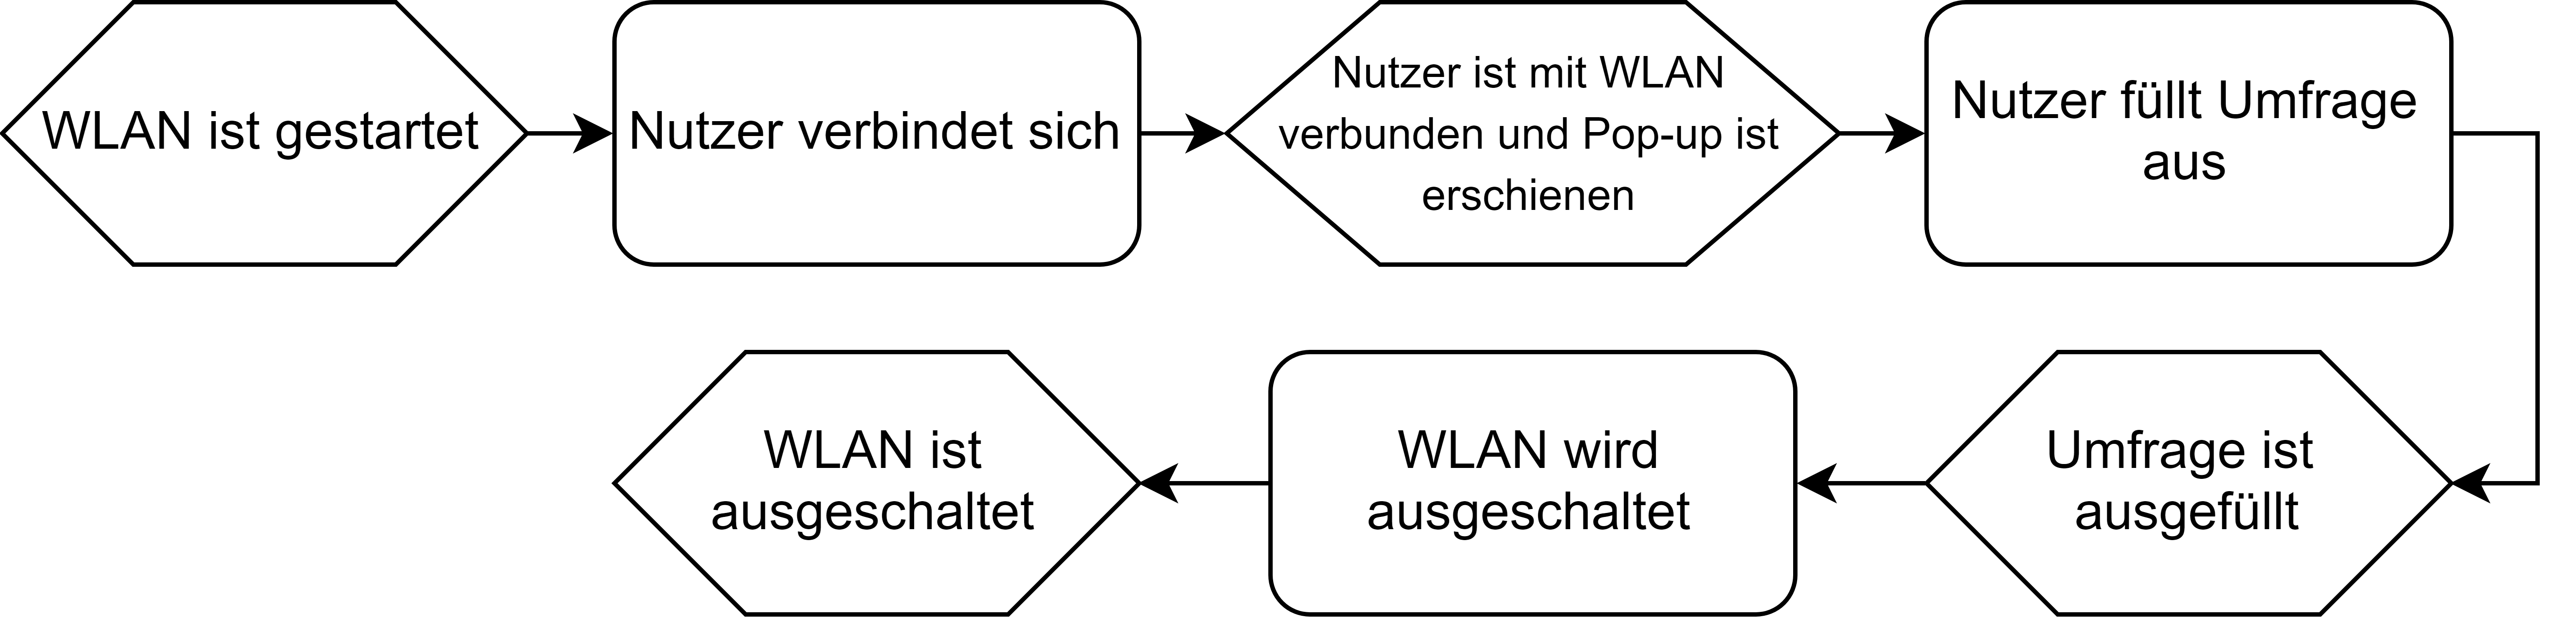
\includegraphics[width=0.9\textwidth]{images/captiveportal_EPK1}
\caption[EPK zum Ablauf ohne Internetzugang]{EPK zum Ablauf ohne Internetzugang}
\label{fig:captive_epk1}
\end{figure}


Die in \ref{fig:captive_epk2} dargestellte EPK zeigt die Verwendung eines Captive Portals mit Internetzugang. Diese Lösung könnte bei einem längerfristigen Einsatz Anwendung finden und während des Umfragezeitraums etwa in der Kantine vor den Internetzugang geschaltet werden. Nachdem sich der Nutzer mit dem WLAN verbunden hat, erscheint auch hier der Pop-up mit der Umfrageseite. Da der Nutzer nicht gezwungen werden darf, diese auszufüllen, kann sie durch einen \textit{Überspringen}-Button übersprungen werden und der Nutzer gelangt direkt ins Internet. Alternativ füllt der Nutzer die Umfrage aus und erhält im Anschluss den Zugang ins Internet. Soll die Umfrage erneut durchgeführt werden, kann der Nutzer - etwa durch einen Timeout - vom WLAN abgemeldet werden und er erhält bei der nächsten Verbindung erneut das Pop-up mit der Umfrageseite und anderen Fragen.

\begin{figure}[H]
\centering
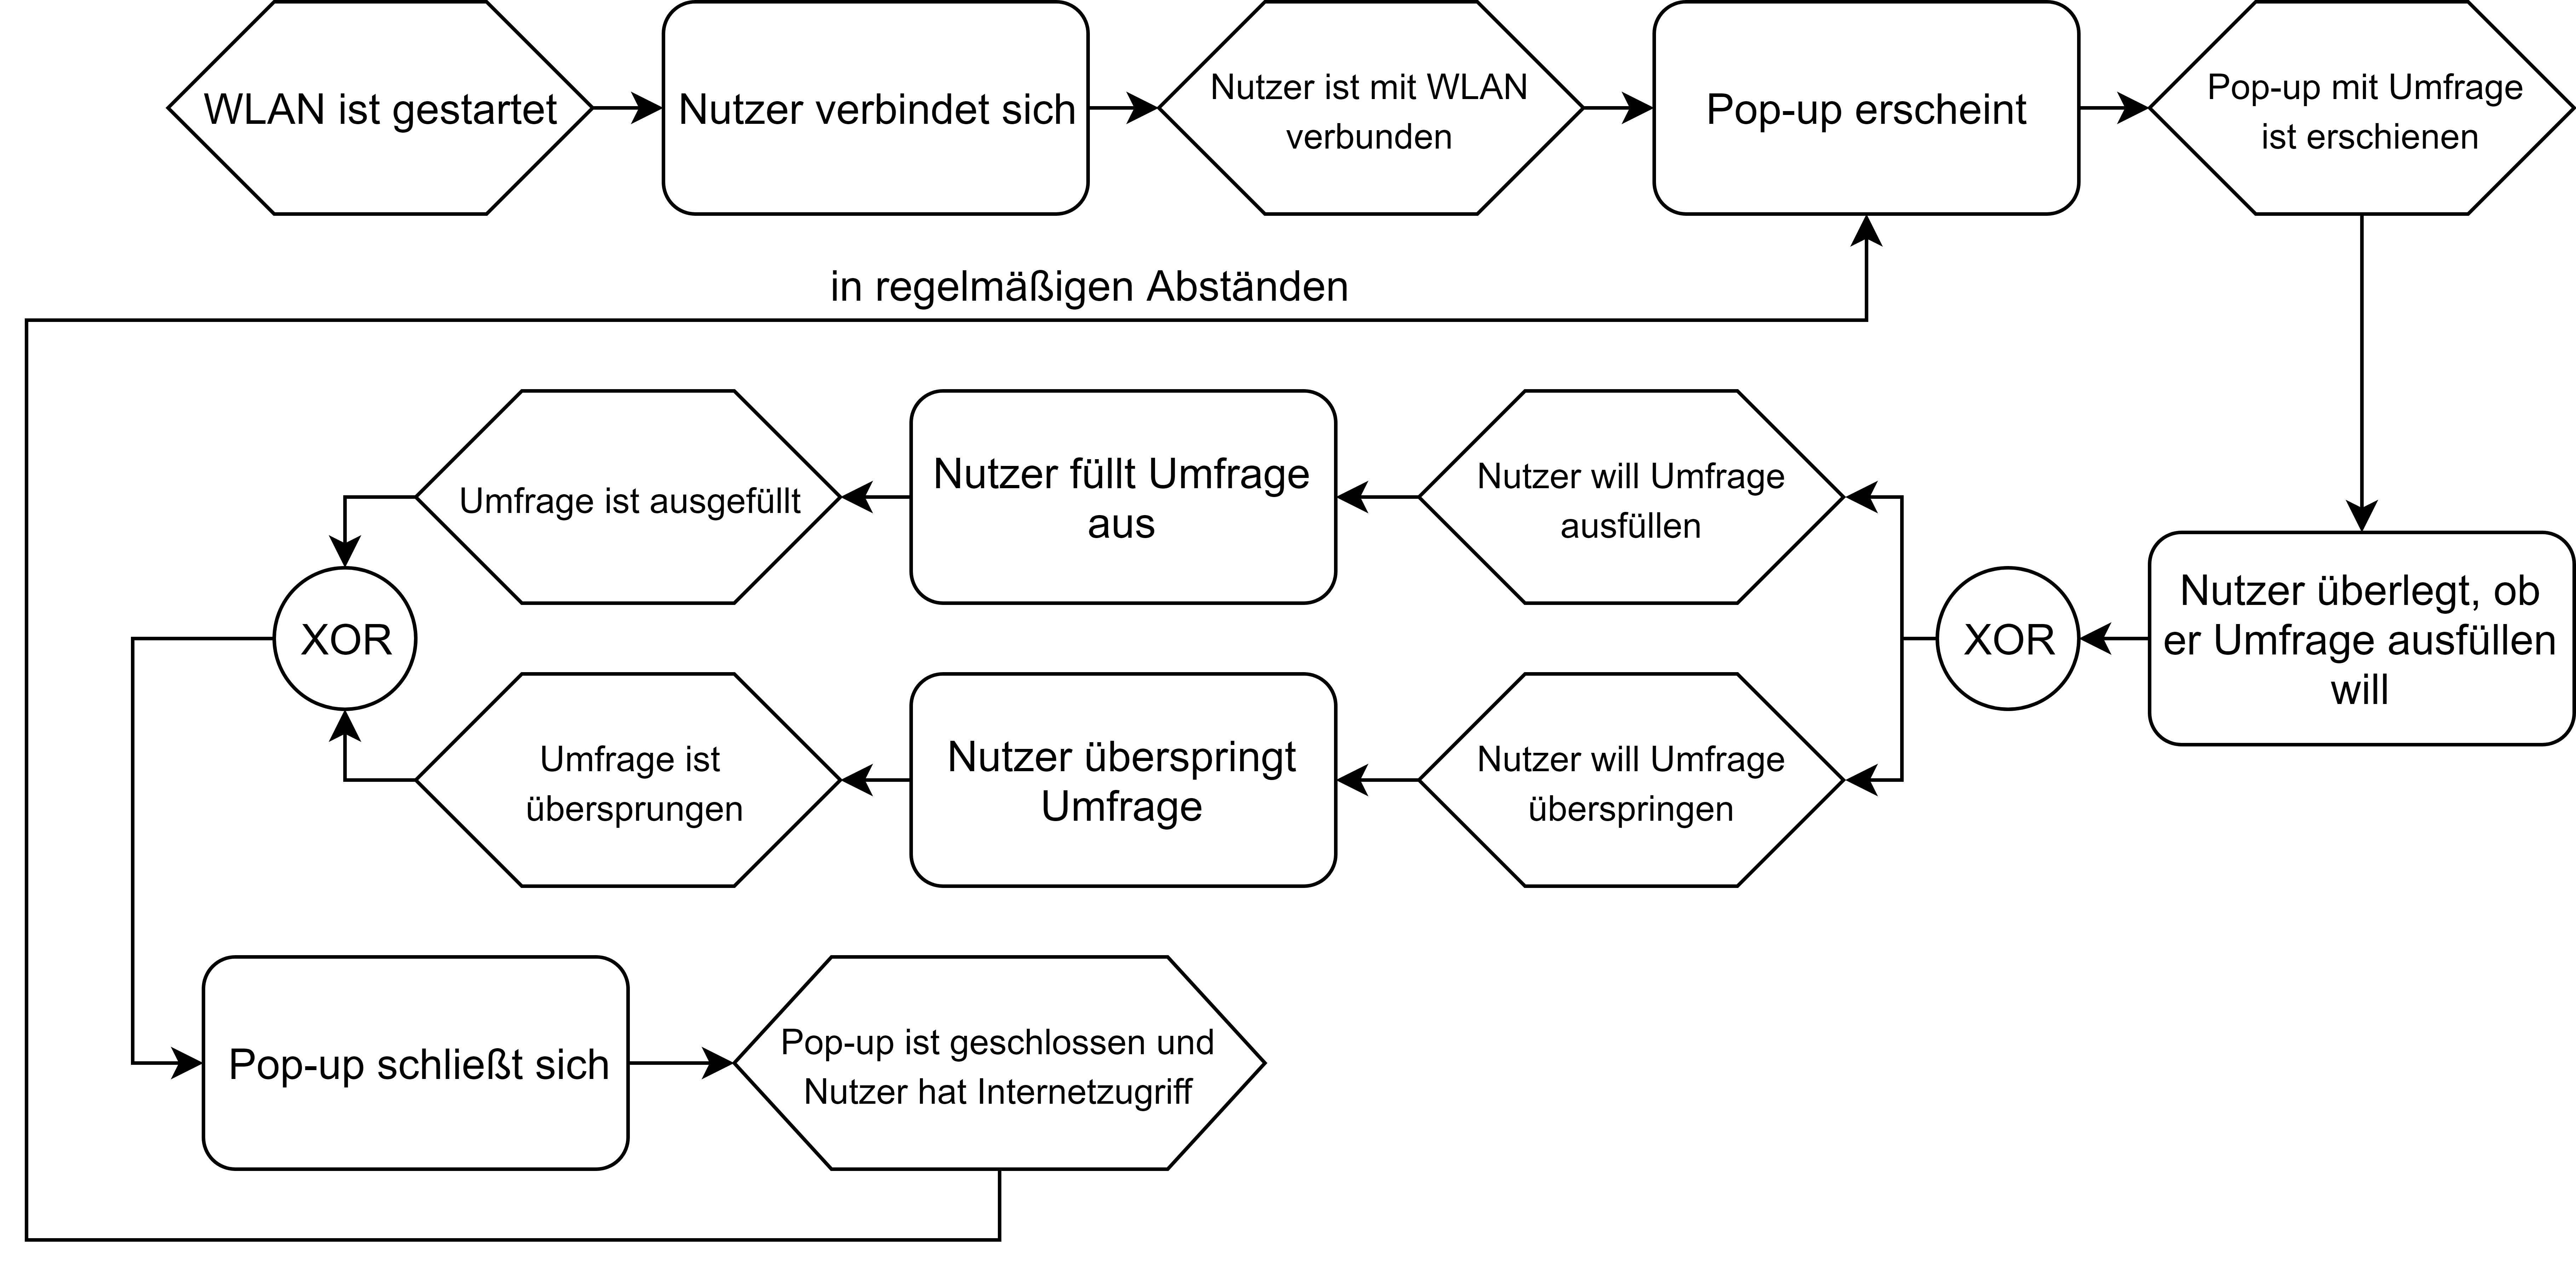
\includegraphics[width=0.9\textwidth]{images/captiveportal_EPK2}
\caption[EPK zum Ablauf mit Internetzugang]{EPK zum Ablauf mit Internetzugang}
\label{fig:captive_epk2}
\end{figure}

 
\subsection{Architektur}
\subsubsection{Verwendung eines Raspberry Pi}
\subsubsection*{Initiale Einrichtung und verwendete Hardware}
Der Raspberry Pi soll die Funktionalität eines Captive Portals für Umfragen veranschaulichen. Grundsätzlich benötigt wird hierfür:
\begin{itemize}
\item Raspberry Pi 3
\item Stromkabel
\item SD Karte
\end{itemize}

Da der Raspberry Pi 3 bereits einen WLAN-Empfänger eingebaut hat, wird kein zusätzlicher WLAN-USB-Empfänger benötigt. Zunächst muss das Betriebssystem Raspbian Stretch auf dem Raspberry Pi  installiert werden. Hierfür kann beispielsweise das Installationsprogramm \textit{NOOBS} genutzt werden, das über einen Computer auf die SD Karte gespielt wird. Anschließend erfolgt die Installation und die Aktualisierung des Betriebssystems durch \textit{apt-get update} und \textit{apt-get upgrade}.

\subsubsection*{Anleitung 1 - Captive Portal ohne Internet}
Um das Captive Portal einzurichten, wird zunächst der Ansatz ohne Internetverbindung, also mit einer lokal gehosteten Webseite, gewählt. Diese eignet sich insbesondere für die Verwendung bei Gesamtveranstaltungen, bei denen die Umfrage einmalig durchgeführt wird. Hierfür wird der unter \textit{https://brennanhm.ca/knowledgebase/2016 /10/raspberry-pi-access-point-and-captive-portal-without-internet/} zu findenden Anleitung gefolgt. Um diese umzusetzen, müssen auf dem Raspberry Pi die Pakete \textit{hostapd} und \textit{dnsmasq} installiert werden.

Das Paket \textit{hostapd} ermöglicht es, dass der WLAN-Empfänger als Access Point dienen kann, also Verbindungen von anderen Endgeräten annimmt. Bei dem Paket \textit{dnsmasq} handelt es sich um einen einfach zu konfigurierenden DNS- und DHCP-Server. Für beide Pakete müssen anschließend weitere Konfigurationen durchgeführt werden.

Das letzte Paket \textit{nginx} bietet einen Webserver, der für das lokale Hosting der Umfrage-Seite genutzt wird. Die in der Anleitung vorgeschlagene \textit{nginx}-Konfiguration wird um das rewrite-Statement für den /feedback/ Pfad ergänzt. In dem Block für den /generate\_204 Pfad können URL-Parameter mitzurückgegeben werden. Diese werden auch auf Android und auf Windows Endgeräten genutzt, bei iOS hingegen funktioniert dies nicht. Aus diesem Grund wurden diese URL-Parameter, nach unterschiedlichen Versuchen, nginx richtig zu konfigurieren, direkt in der JavaScript-Datei der Umfrage-Webseite festgelegt. Der Nutzer wird ebenfalls auf die Umfrageseite weitergeleitet, wenn er eine beliebige URL in seinen Browser eingibt.

Das Captive Portal des Raspberry Pi funktioniert mit dieser Anleitung problemlos auf Windows-Computern, iOS-Endgeräten und den meisten Android-Engeräten. Lediglich bei Samsung-Smartphones öffnet sich der Pop-up zum Anmelden am WLAN nicht. Der Grund hierfür ist nicht klar, könnte jedoch möglicherweise durch eine andere dnsmasq- oder nginx-Konfiguration behoben werden.

Die automatische Einrichtung des Raspberry Pi wird durch ein selbst erstellten Shell Skript ermöglicht, dass die Schritte in der Anleitung hintereinander durchführt. Voraussetzung ist ein neu aufgesetzter Raspberry Pi 3 mit WLAN-Interface wlan0. Der Name des WLAN-Netzwerks wird als Argument \textit{sudo bash setup.sh Name\_des\_WLANs} übergeben, die Webseite muss anschließend in den Ordner /usr/share/nginx/html/host kopiert werden.

\subsubsection*{Anleitung 2 - Captive Portal mit Internet}
Eine zweite Anleitung ermöglicht es, den Raspberry Pi als WLAN-Access Point mit Captive Portal für einen Internetzugang zu nutzen, was für den längerfristigen Einsatz - etwa in einer Kantine - geeignet wäre. Hierfür werden die Anleitungen 2a unter \textit{https://pimylifeup.com/raspberry-pi-wireless-access-point/} für die Einrichtung des Access Points und 2b unter \textit{https://pimylifeup.com/raspberry-pi-captive-portal/} für die Captive Portal Funktionalität genutzt.

Für die Einrichtung des Access Points werden erneut die Pakete \textit{hostapd} und \textit{dnsmasq} genutzt. Zusätzlich werden die IP-Tabellen verändert und diese Veränderungen und ein Neustart von \textit{hostapd} und \textit{dnsmasq} in die rc.local Datei geschrieben, damit diese bei jedem Neustart umgesetzt werden. Dies hat jedoch bei dem Austesten der Anleitung nicht funktioniert, sodass ein \textit{sleep 10} Befehl der rc.local Datei hinzugefügt werden musste.

Im zweiten Schritt wird für den Access Point die Captive Portal Funktionalität hinzugefügt. Hierfür wird die Software \textit{nodogsplash} auf dem Raspberry Pi installiert. Diese hostet lokal die Captive Portal Seite in dem Verzeichnis \textit{/etc/nodogsplash/htdocs/splash.html}. Auf der Captive Portal Seite kann ein Formular abgeschickt werden, mit dem der Nutzer authentifiziert wird und mit dem er Zugriff auf das Internet erhält. Dieses kann zum Überspringen der Umfrage direkt oder erst nach dem Ausfüllen der Anfrage abgeschickt werden. Hierfür müsste der Umfrage-Webapp ein \textit{Überspringen}-Button und ein \textit{Umfrage abschließen}-Button hinzugefügt werden, durch die das Formular abgeschickt wird. In der nodogsplash.conf Datei können weitere Konfigurationen vorgenommen werden, insbesondere auch der Internetzugriff für nicht-authentifizierte Nutzer erlaubt werden, sodass auf der Captive Portal Seite Inhalte aus dem Internet angezeigt werden.

Diese Lösung funktioniert auf allen Endgeräten, insbesondere auch auf denen von Samsung. Liegt kein Internet vor, funktioniert das Captive Portal jedoch nicht. Hierfür muss in der dnsmasq.conf Konfigurationsdatei \textit{address=/\#/IP\_des\_Raspberry} zur Auflösung aller Domainnamen auf den Raspberry Pi hinzugefügt werden. Ist dies erfolgt, funktioniert das automatische Pop-up bei Samsung Smartphones jedoch nicht mehr.

Auch für diese Anleitungen wurden Shell Skripte umgesetzt. Diese können mit \textit{sudo bash setup2a.sh Name\_des\_WLANs Passwort\_des\_WLANs} und \textit{sudo bash setup2b.sh} ausgeführt werden.

\subsubsection*{Weiteres Vorgehen}
Die Umsetzung des Captive Portals mithilfe des Raspberry Pi dient in erster Linie zur Veranschaulichung der Möglichkeit, die Umfrage in dieser Form umzusetzen. Sollte eine der Lösungen des Raspberry Pi tatsächlich in einem produktiven Umfeld genutzt werden, sind folgende Aspekte zu beachten:
\begin{itemize}
\item Es sollte ein externer WLAN-Empfänger genutzt werden, da der in dem Raspberry Pi eingebaute Empfänger vermutlich eine zu geringe Signalstärke hat. In diesem Fall müssten die Konfigurationen entsprechend angepasst werden. Gleichzeitig muss überprüft werden, wie viel Verbindungen gleichzeitig unterstützt werden können.
\item Das Problem der automatischen Pop-ups bei Samsung Handys muss behoben werden, das Problem liegt womöglich an der DNS-Auflösung oder der zurückgegebenen Status-Codes.
\item Die Anleitungen müssen vertieft auf die Aspekte Sicherheit und Performance überprüft werden, möglicherweise auch eine SSL-Verschlüsselung eingerichtet werden. Die Lösungen sollten in der bestehenden Form noch nicht produktiv genutzt werden, da Sicherheitsrisiken bestehen, die insbesondere bei der zweiten, längerfristigen Lösung mit Internetzugang gefährlich sind.

\end{itemize}

\subsubsection{Alternative Ansätze}
Neben der Verwendung des Raspberry Pi gibt es verschiedene Hardware- und Softwarelösungen, die ebenfalls die Captive Portal Funktionalität bieten. Vorteil von diesen ist, dass es sich in der Regel bereits um fertig konfigurierte und funktionierende Lösungen handelt; Nachteil ist hingegen, dass häufig wenig Konfigurationen möglich sind.

Bietet ein Unternehmen seinen Mitarbeitern einen WLAN-Internetzugang an, so wird dieser meist über zentral verwaltete Access Points realisiert. Hier besteht die Möglichkeit, dass der Access Point bereits eine Captive Portal Funktionalität besitzt. Die meiste vorinstallierte Software besitzt jedoch nur die Möglichkeit, eine einfache Webseite zum Akzeptieren der Nutzungsbedingungen anzuzeigen, sodass die eigene Umfrageseite nicht einfach eingebunden werden kann (z.B. nur als Redirect nach dem Akzeptieren der Nutzungsbedingungen). Aus diesem Grund ist es unwahrscheinlich, dass die Umfrageseite als Captive Portal direkt in der Access Point Software eines Unternehmens aktiviert werden kann.

Eine andere Lösung ist es, beispielsweise die Firewall- und Router-Software pfSense vor die Access Points oder bei Gesamtveranstaltungen vor einen eigenen Access Point zu schalten. Diese ermöglicht ebenfalls die Captive Portal-Funktionalität. Der Einsatz ist jedoch in einem Firmennetzwerk er unwahrscheinlich, da ein größerer Eingriff in die Ntzwerkinfrastruktur erforderlich ist.

Als Alternative könnte auch das Betriebssystem eines kompatiblen Routers durch das auf Linux basierende, weit verbreitete Betriebssystem OpenWRT überschrieben werden, um diesen selbst zu konfigurieren. In diesem Fall ähneln die Konfigurationsarbeiten denen auf dem Raspberry Pi und für die Captive Portal Funktionalität kann eine Software wie nodogsplash, Wifidog oder CoovaChilli genutzt werden.




\subsubsection{Anforderungserfüllung}
Die zentralen Anforderungen des Lasten- und Pflichtenhefts wurden erfüllt. Mit der ausgewählten Hardware - einem Raspberry Pi - wurde das Captive Portal prototypisch eingerichtet. Die verwendeten Lösungsansätze können somit als Demo, für praktische Tests (zur Einschätzung, ob dieser Umfragekanal geeignet ist) und als Grundlage für eine spätere produktive Nutzung dienen. Zudem wurden mögliche Probleme, wie etwa die Verwendung von Samsung Endgeräten, aufgedeckt.

Weniger intensiv wurden hingegen die alternativen Lösungsansätze betrachtet, da diese sehr Hardware-abhängig sind und diese Hardware für eine sinnvolle Einschätzung durch Austesten nicht zur Verfügung stand. Aus diesem Grund wurden diese nur konzeptionell beschrieben.


\section{Newsfeed App - Recherchebericht}
\label{section:realisation:newsfeed_app}


Newsfeed App for deskless/frontline employees Firstline workers
\begin{itemize}
\item {Mircosoft Staffhub https://products.office.com/de-de/microsoft-staffhub/staff-scheduling-software}
\item {Inkling 	https://www.inkling.com/ }
\item {Zinc https://www.zinc.it/ Beliebteste/Am häufigsten genutzte App für „Deskless“ Mitarbeiter}
\item {Slack https://slack.com/intl/de-de Desktop worker or/and Frontline worker?}
\item {Nicht geeignet: Whatsapp Business https://www.deutsche-handwerks-zeitung.de/whatsapp-betrieblich-nutzen-was-beim-datenschutz-wirklich-gilt/150/3101/363865}
\end{itemize}


\subsection{Lastenheft}
\begin{itemize}
\item Es ist ein Recherchebericht zu erstellen, der sich mit Produkten, Lösungen und Anwendungen (im Folgenden als Anwendungen zusammengefasst) befasst. Konkret geht es um Anwendungen, die es Unternehmen ermöglichen, ihre Mitarbeiter über unternehmensinterne Vorgänge zu informieren und den Mitarbeitern eine Interaktion mit dem Unternehmen ermöglichen. 
\item Der Bericht soll eine Übersicht über die am Markt etablierten Anwendungen liefern. Ein Fokus soll auf den Anreizen liegen, mit welchen die Anwendungen die Mitarbeiter zur Benutzung motivieren.
\item Des Weiteren soll im Bericht untersucht werden, welche Umfragefunktionalitäten in der jeweiligen Anwendung bereits existieren und wie diese potentiell durch PulseShift genutzt werden könnten. 
\item Darüber hinaus soll der Bericht aufzeigen, welche weiteren Möglichkeiten zur Einbindung einer Umfrage durch PulseShift es jeweils gibt und wie flexibel diese Möglichkeiten genutzt werden können.
\item Außerdem sollen in dem Bericht die Erfahrungen von Referenzkunden, die die Anwendung bei Offline-Mitarbeitern einsetzen, beschrieben werden. 
\item Sofern jeweils eine Preisstruktur verfügbar ist, soll außerdem auf diese eingegangen werden.
\end{itemize}

\subsection{Pflichtenheft}
\begin{itemize}
\item Es wird ein Recherchebericht erstellt, der sich mit Produkten, Lösungen und Anwendungen (im Folgenden als Anwendungen zusammengefasst) befasst. Konkret wird es um Anwendungen gehen, die es Unternehmen ermöglichen, ihre Mitarbeiter über unternehmensinterne Vorgänge zu informieren und den Mitarbeitern eine Interaktion mit dem Unternehmen ermöglichen.
\item Der Bericht wird eine Übersicht über die am Markt etablierten Anwendungen liefern. Für die Marktführer wird herausgearbeitet, mit welchen Anreizen sie die Mitarbeiter zur Benutzung der Anwendung motivieren. Sofern jeweils möglich werden die Anwendungen dazu neben einer Internetrecherche auch aktiv getestet.
\item Des Weiteren werden im Bericht die Möglichkeiten zur Integration der Umfrage von PulseShift in die jeweilige Anwendung aufgezeigt. Diese wird tabellarisch mit zusätzlichen erläuternden Texten gegenübergestellt. Dabei wird sofern jeweils verfügbar sowohl auf die Umfragefunktionalitäten der Anwendung als auch das Abspringen zur Umfragefunktion von PulseShift eingegangen. Außerdem werden jeweils mögliche weitere anwendungsspezifische Möglichkeiten wie beispielsweise ein Einbinden der Umfrage mittels iFrame vorgestellt.
\item Abschließend werden die Erfahrungen von Referenzkunden dargelegt. Dabei wird der Fokus auf Erfahrungen liegen, die im unmittelbaren Zusammenhang mit dem Einsatz bei Offline-Mitarbeitern stehen.
\item Der Bericht wird innerhalb des Projektabschlussberichts in Latex erstellt.
\end{itemize}


\subsection{Firstline Worker}

Die Firstline Workforce klassifiziert alle Mitarbeiter ohne festen Computer-Arbeitsplatz. Sie repräsentieren die mehr als zwei Milliarden Menschen  in Rollen, die sie zum ersten Kontaktpunkt zwischen einem Unternehmen und der Außenwelt machen. Sie sind die Menschen hinter der Theke, am Telefon, in den Kliniken und in der Werkstatt. Sie bilden das Rückgrat vieler der weltweit größten Branchen - Einzelhandel, Restaurants, Gastgewerbe, Reisen, Fertigung und Bauwesen. In dieser Rolle sind sie oft die ersten, die Kunden ansprechen, die ersten, die die Marke eines Unternehmens repräsentieren und die ersten, die Produkte und Dienstleistungen in Aktion sehen.


\begin{figure}[H] 
\centering 
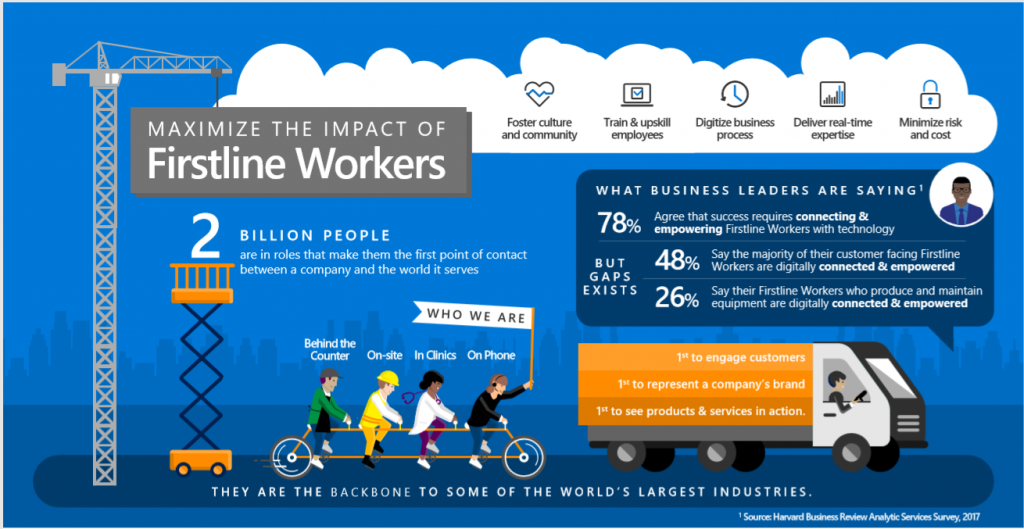
\includegraphics[scale=0.48]{images/frontlineworkers} 
\caption[Frontline Workers]{Firstline workers Aufgabenbereiche\protect} 
\label{dem} 
\end{figure}


\subsection{Microsoft Staffhub}

Microsoft StaffHub ist eine speziell für die Firstline Workforce in Office 365 entwickelte App . Es wurde speziell entwickelt, um die Fähigkeiten, Werkzeuge und Informationen zu liefern, die Firstline Mitarbeiter benötigen, um effektiv zu arbeiten und Spitzenleistungen zu erbringen. Dieser Service kombiniert Terminplanung, Aufgabenverwaltung, Dokumente, Personen und Tools an einem sicheren Ort - mit der Möglichkeit, sich mit anderen arbeitsbezogenen Apps und Ressourcen zu verbinden.
\begin{itemize}
\item Zugriff auf Schichtenplan
\item Kommunikation innerhalb des Teams
\item Zugriff auf wichtige Information übers Handy
\item Manager können Schichtenplan bearbeiten und Informationen verbreiten
\end{itemize}

\subsubsection{Verfügbarkeit}
Microsoft StaffHub ist derzeit verfügbar im Web, iOS und Android. Derzeit ist Staffhub nicht als eigenständiges Projekt sondern nur im Rahmen der folgenden Office 365-Geschäftspläne verfügbar: F 1, E1, E3 und E5. Wenn ein Kunde bereits einen dieser Pläne hat, kann er direkt Microsoft StaffHub verwenden. Der Einstieg ist ganz einfach. Erstanmelder können sich mit ihrem Office-365 Arbeitskonto unter http://staffhub.office.com anmelden. Von dort aus können sie Zeitpläne für ihre Teams erstellen und verwalten, wichtige Ressourcen und Unternehmensnachrichten hochladen und teilen und Firstline Workers einladen um die Anwendung herunterzuladen.

\subsubsection{Schedule \& Task Management}
Das Schedule \& Task Management ermöglicht es dem Manager die Schichten für die Mitarbeiter zuzuweisen, zu aktualisieren und allgemein zu verwalten. Die Mitarbeiter können gleichzeitig untereinander Schichten tauschen und Urlaub beantragen während der Manager stets die komplette Übersicht und Kontrolle bei Änderungen beibehält. 

\begin{figure}[H] 
\centering 
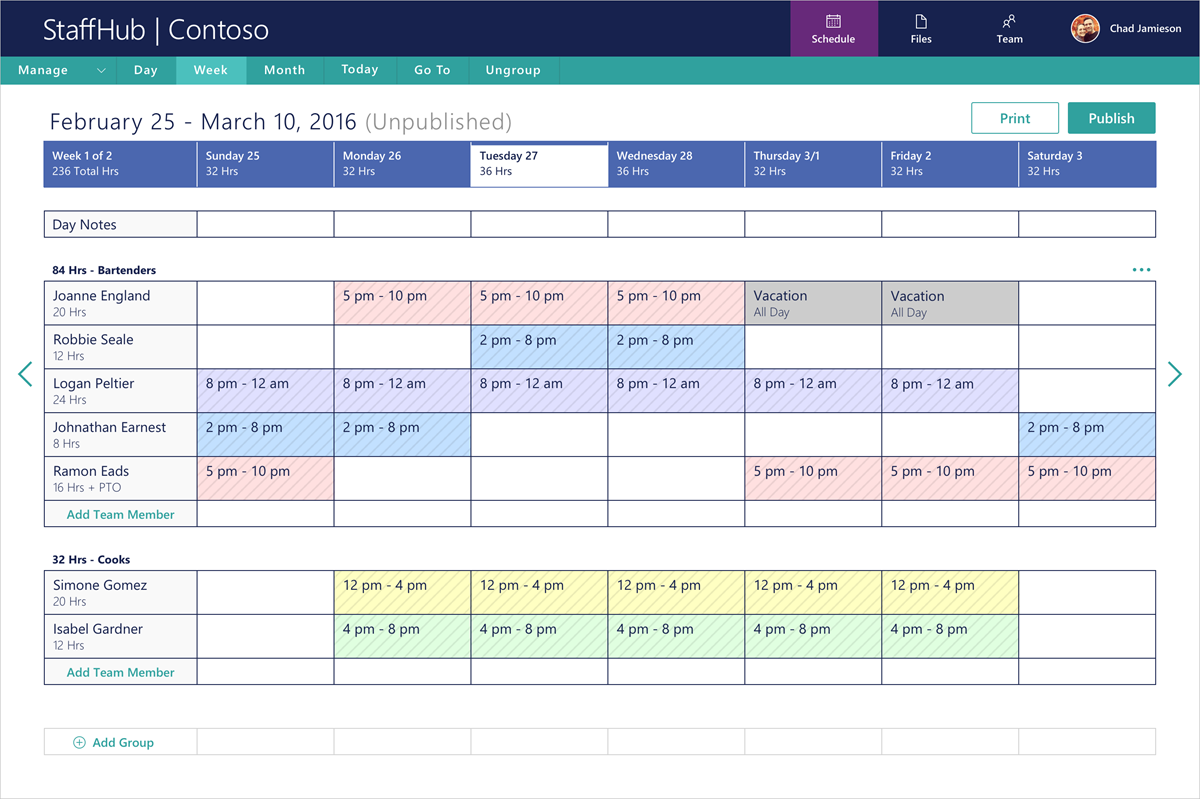
\includegraphics[scale=0.48]{images/schedule} 
\caption[Webansicht Schichtpläne]{Webansicht Schichtpläne\protect} 
\label{ws} 
\end{figure}

\begin{figure}[H] 
\centering 
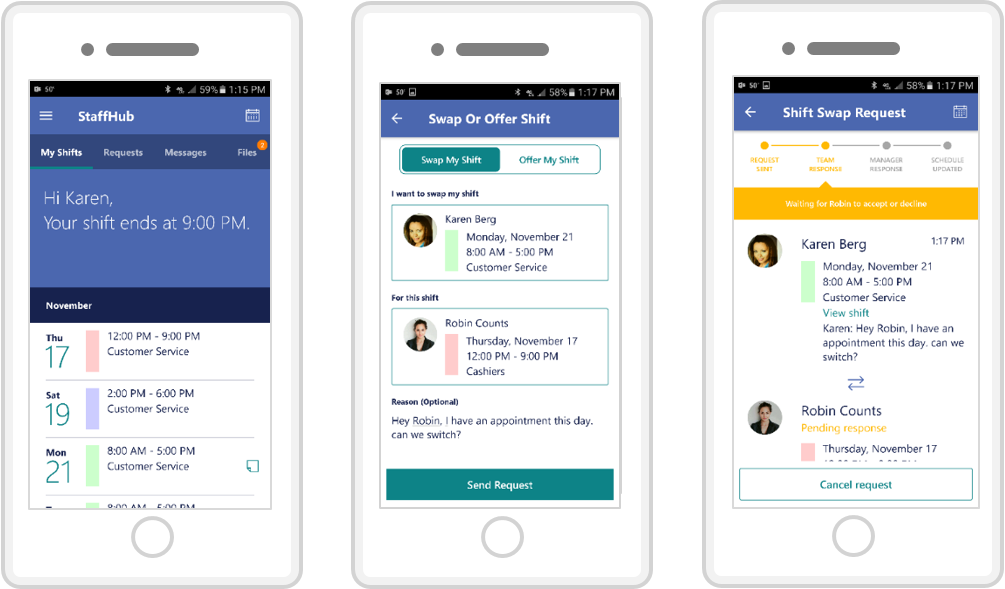
\includegraphics[scale=0.48]{images/schedulemobile} 
\caption[Schichtpläne tauschen mit dem Handy]{Schichtpläne tauschen mit dem Handy\protect} 
\label{ws} 
\end{figure}

Außerdem können einzelne Aufgaben und To-Dos vergeben werden. Diese können direkt durch den Manager vergeben werden oder der Mitarbeiter kann diese selbst als Erinnerung für sich anlegen. 

\begin{figure}[H] 
\centering 
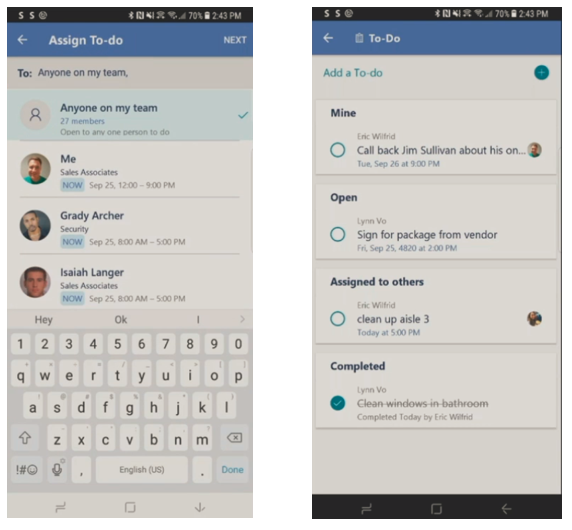
\includegraphics[scale=0.78]{images/todolist} 
\caption[To-Do Liste pflegen]{To-Do Liste pflegen\protect} 
\label{ws} 
\end{figure}

Für die Zukunft ist außerdem geplant mit Hilfe der App eine Zeiterfassung in Realtime zu ermöglichen, sodass nicht mehr klassisch gestempelt werden muss.
Zusätzlich ist es möglich die Funktionalitäten zu erweitern und weitere Services und Apps an Staffhub anzubinden. Zusätzlich ist es möglich die Funktionalitäten zu erweitern und weitere Services und Apps an Staffhub anzubinden.

\subsubsection{Communications \& Community}

In Staffhub können jederzeit neue Kommunikationskanäle aufgesetzt werden, wodurch es möglich ist Gruppen oder persönliche Chats zu starten. Des Weiteren können von dem Unternehmen direkt Best Practices oder Neuigkeiten durch Announcements an den Mitarbeiter kommuniziert werden.

\begin{figure}[H] 
\centering 
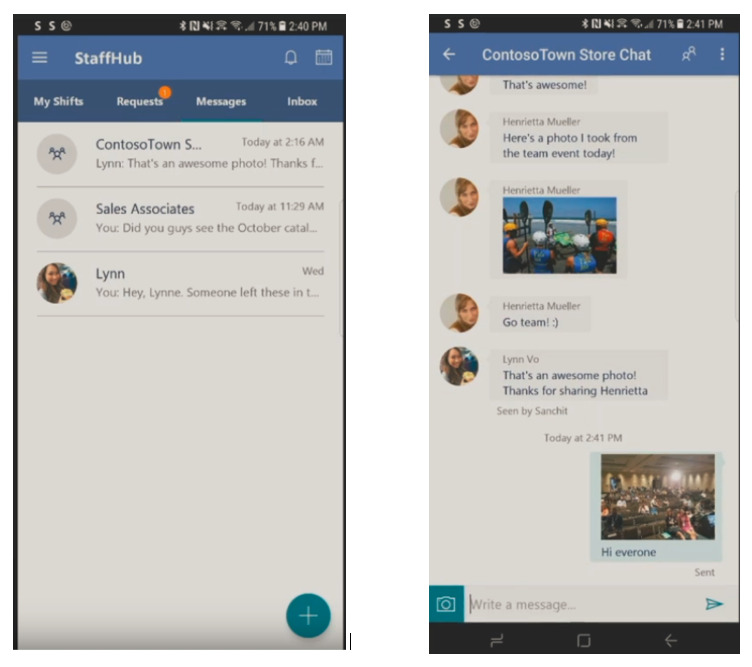
\includegraphics[scale=0.78]{images/groupchat} 
\caption[Teamchats]{Teamchats\protect} 
\label{ws} 
\end{figure}

\subsubsection{Training \& Onboarding}

Mit Staffhub ist es möglich Dokumente und Dateien zu verwalten und innerhalb des Unternehmens zu teilen. Dies wird unter anderem durch die Integration von SharePoint und team sites unterstützt. Auf den Inhalt kann man dabei direkt innerhalb der App zugreifen und dadurch Training und Oboarding Aktivitäten planen.

\begin{figure}[H] 
\centering 
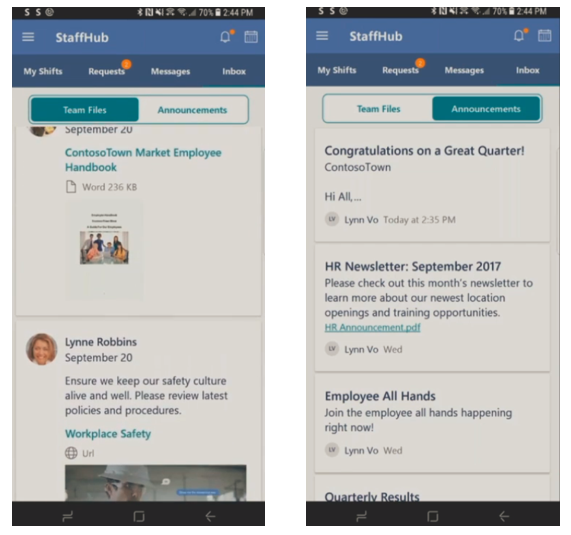
\includegraphics[scale=0.78]{images/communication} 
\caption[File Sharing und Announcements]{File Sharing und Announcements\protect} 
\label{ws} 
\end{figure}

\subsubsection{Identity \& Access Management}

Staffhub ermöglicht die Vergabe von Identitäten mit Hilfe von nur einer Telefonnummer. Eine Email-Adresse ist in diesem Fall optional. Die einzelnen User können dabei zentral mit Office 365 verwaltet werden.

\begin{figure}[H] 
\centering 
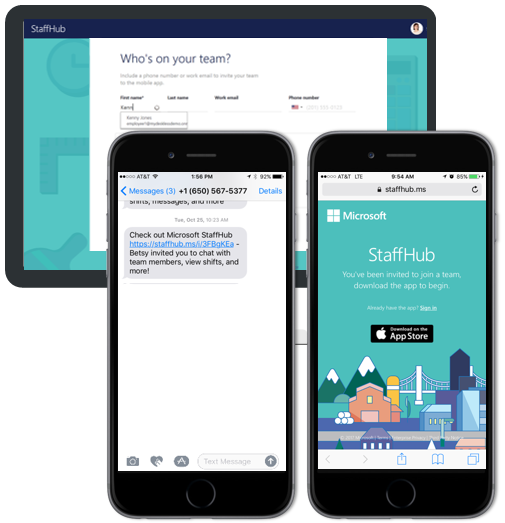
\includegraphics[scale=0.82]{images/invite} 
\caption[Telefonnummer statt E-Mail zur Identifikation]{Telefonnummer statt E-Mail zur Identifikation\protect} 
\label{ws} 
\end{figure}

\subsubsection{API \& Business Integration}

In Staffhub können über die API 3rd Party Lösungen für Workforce Management eingebunden werden. Des Weiteren kann man benutzerspezifische Integration für interne Applikationen und Prozesse hinzufügen. Zusätzlich ist die Integration mit Kronos WorkForce Central V8 unterstützt und es werden Connectors bereitgestellt um mit Microsoft Flow zu arbeiten.
Die API ist nach eigenen Angaben zunächst nur als private Vorschau verfügbar. Jedoch ist eine Erweiterung der API in naher Zukunft geplant und bei weiteren Integrationen und möglichen Partnerschaften kann man sich direkt an staffhubinfo@microsoft.com wenden. Die APIs soll nach einigen Tests und Optimierungen der Öffentlichkeit kostenlos zur Verfügung gestellt werden.

\begin{figure}[H] 
\centering 
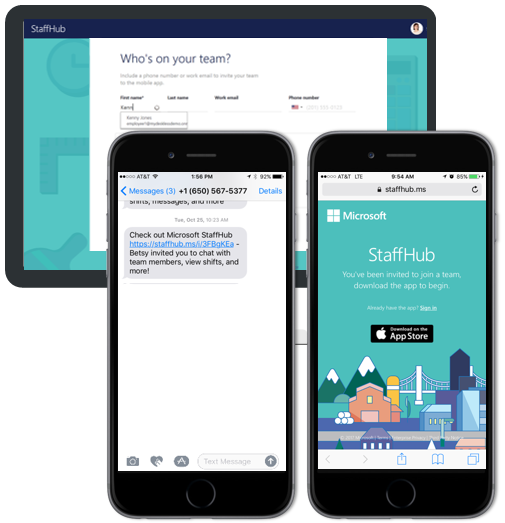
\includegraphics[scale=0.72]{images/invite} 
\caption[Cheat Sheet über Schnittstellen]{Cheat Sheet über Schnittstellen\protect} 
\label{ws} 
\end{figure}

\subsubsection{Unterschied zu Microsoft Teams}
Microsoft Teams ist ein Chat-basierter Arbeitsbereich, der Personen, Unterhaltungen und Inhalte zusammenführt. Microsoft StaffHub ist hingenen eine speziell entwickelte App für die Firstline Workforce zur Verwaltung ihres Arbeitstages. Laut Microsoft ist die Kommunikation für beide wichtig und kündigten kürzlich die Integration von StaffHub Messaging und Microsoft Teams an, um es Firstline Workers zu ermöglichen, sich mit allen Mitarbeitern zu verbinden und zusammenzuarbeiten.
 
\subsubsection{Bewertung}
Insgesamt erweist sich Microsoft Staffhub als sehr umfrangreiches und mächtiges Tool, obwohl es erst vor kurzem für die Öffentlichkeit verfügbar ist. Dadurch besteht die Möglichkeit, dass PulseShift sich die Funktionen von Staffhub zu Nutzen machen kann und die Umfrage in das Tool einzubinden. Dafür gibt es mehrere Optionen: PulseShift kann ein eigenen User beantragen und ist neben allen Mitarbeitern innerhalb des nutzenden Unternehmens zusätzlich als Drittpartei eingebunden. Dies ermöglicht dass PulseShift in einem Teamchat regelmäßig auf die Umfrage aufmerksam machen kann oder die Umfrage zentral an alle Mitarbeiter über ein Announcement verteilen, da es problemlos möglich ist ein Link oder ein Dokument innerhalb der App aufzurufen. Außerdem kann es jedem Nutzer individuell als To-Do Task assigned werden, wodurch der Mitarbeiter sich eher in der Verpflichtung sieht diese Aufgabe auch abzuhaken.
Darüber hinaus besteht mit der API, die in Zukunft weiter ausgebaut wird auch die Umfrage als Applikation von außen über eine Schnittstelle einzubinden.

\subsection{Cotap}
Cotap ist eine von Zinc entwickelte mobile Nachrichtenapplikation für das Unternehmensumfeld. Sie ist insbesondere für \glqq Deskless\grqq Unternehmen geeignet. Es soll dem Unternehmen ermöglichen schnell und einfach mit seinen Mitarbeitern zu kommunizieren. 

Die Funktionalitäten der Applikation lassen sich in zwei Hauptkategorien aufteilen. 

\begin{itemize}
\item Kommunikationstools - zur Kommunikation im Unternehmen 
\item Analysetools - zur Analyse des Kommunikationsverhalten und somit auch zur Analyse der Unternehmenssituation
\end{itemize}

Folgend werden diese Tools aufgegliedert in die einzelnen Funktionsbereiche vorgestellt.

\subsubsection{Kommunikationstools}

\begin{itemize}
\item 1:1 Messages - senden von direkten Nachrichten an jedem aus der Organisation
\item Group Messages - um sich beispielsweise innerhalb einer Abteilung abzustimmen
\item Content Sharing - um Dokumente und weitere wichtige Informationen mit anderen Mitarbeiten zu teilen
\item Hands Free - Nachrichten werden laut vorgelesen und können eingesprochen werden
\item 3RD Party Messaging - Personen, die nicht der eigenen Organisation zugeordnet sind können einfach über die E-Mail-Adresse hinzugefügt werden
\item Push to Talk - Schnelle und einfache Benachrichtigung anderer Mitarbeiter oder Gruppen durch Walkie Taklie Funktion
\item Broadcast - zum Versenden dringender und wichtiger Nachrichten an alle Beteiligten, zusätzliche Funktionalität eines Pop-Ups
\end{itemize}

Die drei letzte Komponenten 3RD Party Messaging, Push to Talk und Broadcast können für unseren Use Case genutzt werden.

3RD Party Messaging kann es PulseShift ermöglichen, über einen Gruppenchat, in welchen sie eingeladen wurden, einen Link zur Umfrage zu posten. So könnten jeweils einzelne Abteilungen gezielt erreicht werden.

Durch Push to Talk kann darauf aufmerksam gemacht werden, dass es eine Umfrage gibt an der man teilnehmen kann. Hier ist es jedoch entscheidend, dass die Übertragung der Nachricht in Tonform und live ist. 

Mit Hilfe des Broadcasts könnte ein Link zur Umfrage versendet werden. So wird dem Mitarbeiter zusätzlich suggeriert, dass es wichtig ist an dieser Umfrage teilzunehmen. 

\subsubsection{Analysetools}
Mit Hilfe der Analysetools werden die gesendeten Nachrichten, hinsichtlich Menge, Inhalt, Länge und weiteren Kriterien analysiert, um weitere Informationen zu generieren. 

Die verschiedenen Analysen werden folgend kurz dargestellt: 

\begin{itemize}
\item Analyse der einzelnen Kommunikationskanäle
\item Historischer Verlauf der Broadcasts
\item Analyse der Anzahl und Größe von gesendeten Nachrichten
\item Networkmap, um zu zeigen wer mit wem kommuniziert
\end{itemize}

Aus diesen Informationen könnte ein Mehrwert für die Umfragen geschlossen werden, dazu wäre jedoch eine komplette Erweiterung des Umfragekonzeptes notwendig und wird daher vorerst verworfen.

\subsubsection{Integrationsmöglichkeiten}
Cotap bietet die Möglichkeit andere Apps zu integrieren, sodass der Nutzer die App nicht verlassen muss, um mit anderen Apps zu interagieren. Mit Hilfe dieser Funktionalität könnten die Umfragen von PulseShift sehr einfach eingebunden werden. 

Außerdem können automatische Benachrichtigungen erstellt werden, um die Mitarbeiter auf die Umfrage hinzuweisen.

\subsubsection{Kosten}
Die App Cotap kann zunächst einmal kostenlos im Playstore herunter geladen werden. Mit Hilfe dieser kostenlosen Version können unbegrenzt Nachrichten gesendet werden, sowie Fotos, Videos und der eigene Standort geteilt werden. Außerdem sind Basic-Integrationen möglich. 

Für 5 Dollar monatlich soll es möglich sein, Audio und Video Anrufe bis zu 100 Minuten pro Nutzer pro Monat zu tätigen und Daten bis zu zwei GB pro User pro Monat zu versenden. In diesem Paket ist außerdem die Gruppenorganisation und Nutzung enthalten. Des weiteren können individuelle Benachrichtigungen erstellt werden.

Das teuerste Paket ist für 10 Dollar pro Monat zu erhalten. Hier können Audio und Video Anrufe bis zu 250 Minuten pro Nutzer pro Monat getätigt werden. Außerdem können unlimitiert Daten versendet und empfangen werden. Nun können Enterprise-files sowie ein Single Sign-One integriert werden. Außerdem wird alles aktiv überwacht und die Analysetools somit genutzt werden.

\subsubsection{Bewertung}
Cotap erscheint als eine gute Möglichkeit, um die Umfragen von PulseShift zu integrieren. Die genaue Zusammenarbeit mit Cotap, PulseShift und dem jeweiligen Unternehmen muss jedoch abgeklärt werden, sowie die genauen Kosten ermittelt werden.


\chapter{Zusammenfassung}


% Anhang der Arbeit
% 
%
\seAppendix{}


%\chapter{Einige wichtige \LaTeX{}-Kommandos}

%  Testdatei f\"ur die Erzeugung von Literaturreferenzen, die den Regeln von Rene Theisen 
%  (Wissenschaftliches Arbeiten, 2009) folgen
%
%
%
\section{Kommandos f\"ur die Erzeugung von Literaturverweisen}

\subsection{Kurzzitierweise mit der Angabe eines Kurztitels}

Das Kommando \verb+\seCite{par1}{par2}{par3}+ erzeugt einen Literaturverweis im Text. 

\begin{seToplist}{\texttt{par1}:}
\item[\texttt{par1}:] Der erste Parameter  definiert einen optionalen Text, der vor dem eigentlichen Literaturverweis ausgegeben 
                               wird, typischerweise Vgl. oder vgl.
\item[\texttt{par2}:] Der zweite Parameter  wird verwendet, um (z.\,B.) zus\"atzliche Seitenangaben f\"ur den Literaturverweis 
                              vorzunehmen.
\item[\texttt{par2}:] Der dritte Parameter ist der entsprechende Schl\"ussel in der .bib-Datei, in der die Literaturquellen 
                              beschrieben sind (vgl. \texttt{wa.bib}).                                                                                       
\end{seToplist}

Als Beispiel f\"ur die Verwendung des \verb+\seCite+-Befehls dient folgendes Zitat: \glqq{}Die \textbf{Funktion} eines 
Anhangs einer wissenschaftlichen Arbeit wird sehr h\"aufig \textbf{missdeutet}, der Anhang selbst nicht selten \textbf{mi{\ss}braucht}.\grqq{} 
(\seCite{vgl.}{S. 170}{The:WA}).

Bei der von Theisen vorgeschlagenen Zitierweise erfolgt die Angabe der Literaturverweise in der Regel innerhalb einer Fu{\ss}note. 
Hierf\"ur kann das Kommando \verb+\seFootcite+ verwendet werden, das dieselben Parameter wie \verb+\seCite+ besitzt. 

Als Beispiel f\"ur ein indirektes Zitat l\"asst sich die Aussage von Theisen anf\"uhren, dass Hauptinhalte eines (berechtigten) Anhangs erg\"anzende 
Materialien und Dokumente sind, die weitere themenbezogene Informationen liefern k\"onnen.\seFootcite{Vgl.}{S. 171}{The:WA}

Weder das \verb+\seFootcite+- noch das \verb+\footnote+-Kommande k\"onnen bei Gleitobjekten (Verwendung der \verb+figure+-, \verb+table+- oder 
\verb+programm+-Umgebung) verwendet werden. Ein kleiner Workaround, um \LaTeX{} doch dazu zu bringen, Fu{\ss}noten bei Gleitobjekten 
zu akzeptieren, ist in \vref{gleitobjekte} zu finden.

\input{\seWaPathText/se-zitieren-harvard}

\subsection{Verwendung von URLs}

URLs k\"onnen in der \texttt{bib}-Datei mit \texttt{@WWW} definiert werden. Das Feld \texttt{author} ist zwar optional, sollte aber immer angegeben 
werden, da andernfalls im Literaturverzeichnis der Kurztitel nicht ausgegeben wird. Wenn kein Autor bekannt ist, wird die Abk\"urzung o.\ V. verwendet.
Beim Eintrag in der \texttt{bib}-Datei ist zu beachten, dass diese Abk\"urzung zus\"atzlich eingeklammert werden muss, d.\,h. sie ist in der 
Form \texttt{author = \{\{o.~V.\}\}} anzugeben. 

Das Layout der URL-Angabe im Literaturverzeichnis kann \"uber vier Parameter beeinflusst werden.  
In der Datei \texttt{wa-konfiguration-deutsch.tex} k\"onnen Redefinitionen vorgenommen werden.

\begin{seList}
\item \verb+\biburlprefix+ \newline Text, der vor dem eigentlichen URL-Eintrag ausgegeben wird \newline Standardwert: \glqq{}\jblangle{}URL: \grqq{}
\item \verb+\biburlsuffix+ \newline Text, der hinter dem eigentlichen URL-Eintrag ausgegeben wird \newline Standardwert: \glqq{}\jbrangle{}\grqq{}
\item \verb+\bibbudcsep+ \newline Text zwischen dem eigentlichen URL-Eintrag und der Datumsangabe f\"ur den letzten Zugriff auf die URL
                                         \newline Standardwert: \glqq{} -- \grqq{}
\item \verb+\urldatecomment+ \newline Text, der vor der Datumsangabe f\"ur den letzten Zugriff ausgegeben wird
                                          \newline Standardwert: \glqq{}Zugriff am\grqq{}
\end{seList}

Und hier kommen noch zwei Beispiele f\"ur die Angabe von Literaturreferenzen, deren Quelle eine URL ist:
Das Paket \texttt{jurabib.sty} wurde von Jens Berger entwickelt.\seFootcite{Vgl.}{}{Ber:Hoj} 
\glqq{}Google will seine Suche auch in Deutschland um eine Datenbank mit abgesicherten Fakten, Biografien und Bildern erweitern, 
den Knowledge Graph.\grqq{}\seFootcite{}{}{GKN}


\newcommand{\dateiAbk}{\texttt{wa-abkuerzungen.tex}}
%
% Ein kleiner Text, um Abk\"urzungen, Symbole und Glossareintr\"age zu testen
%
%
\section{Kommandos f\"ur die Erzeugung von Abk\"urzungen, Symbolen und Glos\-sar\-eint\-r\"a\-gen}

\subsection{Definition von Abk\"urzungen, Symbolen und Glossareintr\"agen}

Um eine einheitliche Darstellung von Abk\"urzungen, Symbolen und Glossareintr\"agen zu erreichen, 
werden vier neue Kommandos zur Verf\"ugung gestellt:

\begin{seList}
\item 
\verb+\seNewAcronymEntry+\newline
Definition einer neuen Abk\"urzung.
\item 
\verb+\seNewSymbolEntry+\newline
Definition eines neuen Symbols.
\item
\verb+\seNewGlossaryEntry+\newline
Definition eines neuen Eintrags im Glossar.
\item
\verb+\seNewAcronymGlossaryEntry+\newline
Definition eines neuen Eintrags im Glossar, wobei zus\"atzlich eine 
Abk\"urzung definiert wird, die dann auch in das Abk\"urzungsverzeichnis aufgenommen wird.
\end{seList}

Der Datei \dateiAbk{} lassen sich die zugeh\"origen \textbf{Pa\-ra\-me\-ter\-be\-schrei\-bun\-gen}  
entnehmen.
In dieser Datei sind auch Beispiele enthalten, wie Abk\"urzungen, Symbole und Glossareintr\"age mit den 
Standardkommandos definiert werden k\"onnen, was jedoch nicht empfohlen wird!

\subsection{Verwendung von Abk\"urzungen, Symbolen und Glossareintr\"agen im Text}

Innerhalb des Textes wird f\"ur Abk\"urzungen, Symbole und Glossareintr\"age das Kommando \verb+\gls{par1}+ 
verwendet.
\texttt{par1} stellt einen Schl\"ussel dar, der die entsprechende Definition identifiziert (vgl. den Inhalt der Datei
\dateiAbk{}). 

Mit dem Kommando \verb+\glspl+ ist es m\"oglich, beim
Auftreten eines Begriffes,  f\"ur den ein Glossareintrag existiert, bzw.\ beim (ersten) Auftreten einer 
Abk\"urzung f\"ur die Vollform die  \textbf{Pluralform} auszugeben.%
\footnote{Genauer gesagt wird derjenige Wert ausgegeben, der in den 
Kommandos \texttt{\textbackslash{}seNewAcronymEntry}, \texttt{\textbackslash{}seNewGlossaryEntry} bzw. \texttt{\textbackslash{}seNewAcronymGlossaryEntry}
als Pluralform definiert wurde. Die Pluralform k\"onnte man alternativ verwenden, um beispielsweise eine 
Genitivform zu definieren.}

Bei den Kommandos 
\begin{seList}
\item\verb+\seNewAcronymEntry+ und 
\item\verb+\seNewAcronymGlossaryEntry+
\end{seList}
kann durch die Verwendung des optionalen Parameters 
zu\-s\"atz\-lich eine Pluralform f\"ur die Abk\"urzung definiert werden (vgl. \dateiAbk{}).

\subsection{Anwendungsbeispiele}

\subsubsection{Abk\"urzungen}

Die dreimalige Anwendung von \verb+\gls{usb}+ liefert:

\begin{seList}
\item \gls{usb}
\item \gls{usb}
\item \gls{usb}
\end{seList}

Die Anwendung von \verb+\glspl{dm}+ \verb+\glspl{dm}+ \verb+\gls{dm}+ liefert:

\begin{seList}
\item \glspl{dm}
\item \gls{dm}
\item \gls{dm}
\end{seList}

Und auch die \gls{dhbw} soll noch erw\"ahnt werden, um das Abk\"urzungsverzeichnis ein wenig zu f\"ullen.

\subsubsection{Symbole}

Bei einem Symbol wird -- im Gegensatz zu Abk\"urzungen -- beim ersten Auftreten im Text nicht die 
zugeh\"orige Definition ausgegeben. Diese ist aber im Symbolverzeichnis zu finden.

Die zweimalige Anwendung von \verb+\gls{pi}+ liefert:

\begin{seList}
\item \gls{pi}
\item \gls{pi}
\end{seList}

Und jetzt kommt noch ein zweites Symbol f\"ur das Symbolverzeichnis: \gls{ND}

\subsubsection{Glossareintr\"age}

Bei einem Glossareintrag wird beim ersten Auftreten des Begriffes im Text dieser mit \textsuperscript{GL} markiert.
Im Glossar sind die Seitenzahlen angegeben, auf denen der Begriff verwendet wurde. 

Die dreimalige Anwendung von \verb+\gls{glos:AD}+ liefert:

\begin{seList}
\item \gls{glos:AD}
\item \gls{glos:AD}
\item \gls{glos:AD}
\end{seList}

Und hier kommt noch ein Beispiel f\"ur einen Glossareintrag, f\"ur den beim ersten und dritten Auftreten die Pluralform verwendet 
wird:  \verb+\glspl{glos:bs}+  \verb+\gls{glos:bs}+  \verb+\glspl{glos:bs}+ 

\begin{seList}
\item \glspl{glos:bs}
\item \gls{glos:bs}
\item \glspl{glos:bs}
\end{seList}

\subsubsection{Glossareintrag mit einem zus\"atzlichen Eintrag im Ab\-k\"ur\-zungs\-ver\-zeich\-nis}

Nach der ersten Anwendung des Begriffes, f\"ur den ein Glossareintrag erzeugt wurde, wird in der Folge 
jeweils nur noch die Abk\"urzung benutzt. 

Die Kommandoausf\"uhrungen \verb+\glspl{glos:ma}+ \verb+\gls{glos:ma}+  \verb+\glspl{glos:ma}+ haben als 
Ergebnis:

\begin{seList}
\item \glspl{glos:ma}
\item \gls{glos:ma}
\item \glspl{glos:ma}
\end{seList}

\newpage
Und jetzt wird auf einer neuen Seite nochmals \verb+\gls{glos:ma}+ verwendet, um im Glossar die neu hinzugekommene 
Seitennummer zu demonstrieren: \gls{glos:ma}

\subsubsection{Pluralform von Abk\"urzungen}

\textbf{\textsf{Definition einer Abk\"urzung}}

Der Eintrag wurde wie folgt definiert (vgl. \dateiAbk{}):

\vspace{-\baselineskip}
\begin{verbatim}
   \seNewAcronymEntry[URLs]{url}{URL}{Uniform Resource Locator}%
   {Uniform Resource Locators}
\end{verbatim}
\vspace{-\baselineskip}

Die Kommandoausf\"uhrungen \verb+\glspl{url}+ \verb+\gls{url}+  \verb+\glspl{url}+ haben als 
Ergebnis:

\begin{seList}
\item \glspl{url}
\item \gls{url}
\item \glspl{url}
\end{seList}

\seVsd
\textbf{\textsf{Definition eines Glossareintrags mit zus\"atzlicher Abk\"urzung}}

Der Eintrag wurde wie folgt definiert (vgl. \dateiAbk{}):

\vspace{-\baselineskip}
\begin{verbatim}
   \seNewAcronymGlossaryEntry[TAen]{glos:ta}{TA}{Transaktion}%
   {Transaktionen}%
   {Was eine Transaktion ist, sollten Sie ebenfalls bereits wissen!}
\end{verbatim}
\vspace{-\baselineskip}


Die Kommandoausf\"uhrungen \verb+\glspl{glos:ta}+ \verb+\gls{glos:ta}+  \verb+\glspl{glos:ta}+ haben als 
Ergebnis:

\begin{seList}
\item \glspl{glos:ta}
\item \gls{glos:ta}
\item \glspl{glos:ta}
\end{seList}

%2013-07-08
\subsubsection{Literaturverweise in Glossareinträgen}

Auch bei Glossareinträgen müssen natürlich Literaturverweise angegeben werden. 
Wird eine Literaturquelle erstmalig in einem Glossareintrag verwendet, dann tritt das Problem auf, 
dass sie von BibTeX nicht gefunden wird. Ein \textsl{Workaround} besteht darin, für die entsprechenden 
Literaturverweise \verb+\nocite{key}+-Kommandos anzugeben. \verb+key+ ist hierbei der zugehörige Schlüssel 
des Eintrags in der .bib-Datei.\footnote{Achtung: Ein \texttt{\textbackslash{}nocite}-Kommando sollte nur in absoluten Ausnahmefällen 
eingesetzt werden, da hiermit Einträge im Literaturverzeichnis erzeugt werden können, für die (möglicherweise) kein 
Literaturverweis innerhalb der Arbeit existiert.}

\newpage

 

\section{Fu{\ss}noten}

\subsection{Verwendung dreistelliger Fu{\ss}noten}

Bei dreistelligen Fu{\ss}noten tritt das Problem auf, dass der Abstand zwischen Fu{\ss}notennummer und folgendem Text nicht mehr ausreicht.
Der Abstand kann wie folgt vergr\"o{\ss}ert werden:

\begin{seList}
\item
In der Style-Datei \texttt{se-jb-footmisc.sty} wird \"uber \newline \texttt{\textbackslash{}setlength\textbackslash{}footnotemargin\{0.3cm\}} genau dieser Abstand definiert.
\item
\"Andert man den Wert z.\,B.\ auf 0.5cm, dann sollte es auch f\"ur dreistellige Fu{\ss}noten ausreichen.
\end{seList}

\subsection{Fu{\ss}noten in Abbildungen, Tabellen und Programmlistings}

\LaTeX{} erlaubt generell nicht die Verwendung des Kommandos \verb+\footnote+ in \textsl{Gleitobjekten} (\textsl{Floats}). 
Zu den Gleitobjekten geh\"oren \textsl{Abbildungen}, \textsl{Tabellen} und auch \textsl{Programmlistings}. In \vref{fussnote} findet ein 
kleiner \textsl{Workaround} Anwendung, wie man doch Fu{\ss}noten in Gleitobjekten angeben kann. 

\begin{seList}
\item Mit \verb+\footnotemark+ wird in dem \verb+\caption+-Kommando die \textsl{Fu{\ss}notennummer} erzeugt.
\item Mit dem Kommando \verb+\footnotetext+ wird au{\ss}erhalb der Umgebung, die das Gleitobjekt definiert (z.\,B. die 
\verb+figure+-Umgebung), der Text der Fu{\ss}note festgelegt. Hierbei ist zu beachten, dass ein Gleitobjekt auf die n\"achste Seite 
verschoben werden kann. In einem derartigen Fall sollte der Fu{\ss}notentext an einer Stelle im \LaTeX-Quelltext positioniert werden, die ebenfalls zu dieser Seite geh\"ort.\footnote{Standardm\"a{\ss}ig wird man \texttt{\textbackslash{}footnotetext} direkt hinter dem Gleitobjekt definieren, um sicherzustellen,
dass der Fu{\ss}notentext auch der richtigen Fu{\ss}notennummer zugeordnet wird.}
\end{seList}


\section{Abbildungen, Tabellen und Programmlistings\label{gleitobjekte}}

Ein Rechteck besitzt die in \vref{abb1} dargestellte Struktur.

\begin{figure}[htbp]
\centering
\setlength{\unitlength}{1mm}
\begin{picture}(100,30)
\put(0,0){\framebox(100,30){Ich bin kein Quadrat!}}
\end{picture}
\caption[Die Darstellung eines Rechtecks]{Die Darstellung eines Rechtecks\label{abb1}\footnotemark}
\end{figure}
%\footnotetext{\seCite{Vgl.}{S. 400}{The:WA}. Achtung: Dieser Literaturverweis ist  rein fiktiver Natur, 
%die Seite 400 existiert in \seCite{}{}{The:WA} nicht!}\label{fussnote}

Der optionale Parameter im folgenden \verb+\caption+-Kommando
\footnotetext{\seCite{Vgl.}{S. 400}{The:WA}. Achtung: Dieser Literaturverweis ist  rein fiktiver Natur, 
die Seite 400 existiert in \seCite{}{}{The:WA} nicht!}\label{fussnote}


\vspace*{-\baselineskip}
\begin{verbatim}
\caption[Die Darstellung eines Rechtecks]%
{Die Darstellung eines Rechtecks\label{abb1}\footnotemark}
\end{verbatim}
\vspace*{-\baselineskip}

definiert den Eintrag f\"ur das Abbildungsverzeichnis. Dort sollte die Fu{\ss}notennummer nicht auftauchen.
Nutzt man den optionalen Parameter nicht, ist es notwendig,  vor \verb+\footnotemark+ noch ein \verb+\protect+ 
einzuf\"ugen, da \LaTeX{} andernfalls die \"Ubersetzung mit einer Fehlermeldung abbricht. 

Eine Notentabelle kann wie in \vref{noten} dargestellt aussehen.

\begin{table}[htbp]%
\centering%
\begin{tabular}{| c | c |}
\hline
Matrikelnummer & Note \\
\hline
\hline
1234567 & 2,7 \\
\hline
2323456 & 3,5 \\
\hline
9865783 & 1,0 \\
\hline
\end{tabular} 
\caption{Ergebnisse der Klausur Programmierung I\label{noten}}
\end{table}


Eines der wichtigsten Java-Programme \"uberhaupt ist in \vref{hello} zu sehen.

\begin{programm}[htbp]
\begin{lstlisting}
public class HelloDHBW {
  public static void main ( String[] args ) {
    System.out.println ( "Hello DHBW" );
  } // main
} // HelloDHBW
\end{lstlisting}
\caption{Die Klasse \texttt{HelloDHBW}\label{hello}}
\end{programm}



\newpage
% J\"org Baumgart
% 2012-06-01
%
%
\section{Definition und Erzeugung von Querverweisen}

Die Grundlage f\"ur die Erzeugung eines Querverweises bildet die Definition eines 
\textbf{Labels}, z.\,B. \verb+\label{querverweis1}+\label{querverweis1}.

Mit dem Kommando \verb+\vref+, z.\,B. \verb+\vref{querverweis1}+, wird ein Querverweis mit 
den beiden folgenden Eigenschaften erzeugt:

\begin{seList}
\item 
Falls sich das Label auf eine \textsl{Abbildung}, eine \textsl{Tabelle}, ein \textsl{Listing} oder eine 
\textsl{Gleichung} bezieht, wird zus\"atzlich zur entsprechenden Nummer ein Text mit ausgegeben.
Beispielsweise erzeugt \verb+\vref{noten}+ \vref{noten}. Die zugeh\"origen Labels sind dann innerhalb 
der \verb+figure+-, \verb+table+-, \verb+programm-+ oder \verb+equation+-Umgebung definiert. 
Die auszugebenden Texte k\"onnen in der Datei\newline
\hspace*{\fill}\verb+wa-konfiguration-deutsch.tex+\hspace*{\fill}\newline  
umdefiniert werden.

Bezieht sich ein Label auf eine Textstelle, z.\,B. \verb+\label{querverweis1}+, dann wird die Kapitelnummer 
mit dem Zusatz \textsl{Kapitel} ausgegeben: \vref{querverweis1}\newline
F\"ur die Gliederungsebenen \verb+\chapter+, \verb+\section+, \verb+\subsection+, \verb+\subsubsection+ 
und \verb+\paragraph+ kann dieser \textsl{Zusatz} ebenfalls in der Datei \newline
\hspace*{\fill}\verb+wa-konfiguration-deutsch.tex+\hspace*{\fill}\newline 
umdefiniert werden. 
\item
Wenn sich der Querverweis auf die aktuelle Seite bezieht, dann wird keine Seitennummer ausgegeben.
\end{seList}

Bei der Verwendung des \verb+\vref+-Kommandos ist zu beachten, dass vor dem auszugebenden Text ein Leerzeichen 
eingef\"ugt wird. Im Normalfall hat dieses keine weitere Auswirkung. Wenn allerdings ein Absatz direkt mit einem 
\verb+\vref+-Kommando beginnt, dann wird der entsprechende Text nicht linksb\"undig ausgegeben, d.\,h. es liegt 
eine Verletzung des Blocksatzes vor.%

\vref{noten} stellt einen blocksatzverletzenden Querverweis dar.

Dieses \textsl{Problem} l\"asst sich durch die Anwendung des \verb+\vref*+-Kommandos vermeiden.\label{vrefstern} 

\vref*{noten} stellt einen nicht blocksatzverletzenden Querverweis dar.

Allerdings f\"uhrt die Verwendung des \verb+\vref*+-Kommandos innerhalb eines Satzes auch wieder 
zu einem nicht gew\"unschten Ergebnis: Das in \vref*{noten} dargestellte Klausurergebnis ... .%
\footnote{Der Grund, warum die Kommandos \texttt{\textbackslash{}vref} 
und \texttt{\textbackslash{}vref*}
in dieser Form definiert wurden, erschlie{\ss}t sich dem Autor dieses Dokuments allerdings nicht!}

Mit dem Kommande \verb+\pageref+ wird lediglich die Seitennummer ausgegeben, z.\,B. \verb+\pageref{noten}+ \pageref{noten}
oder \verb+\pageref{querverweis1}+ \pageref{querverweis1}.




\section{Definition und Anwendung von zwei neuen Listenumgebungen}

\subsection{Das Layout der Standardlistenumgebung von \LaTeX}

Stichpunktlisten werden in \LaTeX{} mit der \verb+itemize+-Umgebung erzeugt. 
Die Stichpunktliste 

\begin{itemize}
\item 1. Stichpunkt der ersten Ebene
\begin{itemize}
\item 1. Stichpunkt der zweiten Ebene
\item 2. Stichpunkt der zweiten Ebene
\begin{itemize}
\item 1. Stichpunkt der dritten Ebene
\item 2. Stichpunkt der dritten Ebene
\begin{itemize}
\item 1. Stichpunkt der vierten Ebene
\item 2. Stichpunkt der vierten Ebene
\end{itemize}
\end{itemize}
\end{itemize}
\item 2. Stichpunkt der ersten Ebene
\item 3. Stichpunkt der ersten Ebene
\end{itemize}

wird durch die folgenden Anweisungen erreicht:

\vspace*{-\baselineskip}

\begin{verbatim}
\begin{itemize}
\item 1. Stichpunkt der ersten Ebene
\begin{itemize}
\item 1. Stichpunkt der zweiten Ebene
\item 2. Stichpunkt der zweiten Ebene
\begin{itemize}
\item 1. Stichpunkt der dritten Ebene
\item 2. Stichpunkt der dritten Ebene
\begin{itemize}
\item 1. Stichpunkt der vierten Ebene
\item 2. Stichpunkt der vierten Ebene
\end{itemize}
\end{itemize}
\end{itemize}
\item 2. Stichpunkt der ersten Ebene
\item 3. Stichpunkt der ersten Ebene
\end{itemize}
\end{verbatim}

\subsection{Die neue Listenumgebung \texttt{seList} f\"ur Stichpunktlisten}

Weder die Einr\"uckung der einzelnen Ebenen noch die gro{\ss}en Abst\"ande zwischen den einzelnen Stichpunkten sind bei der \verb+itemize+-Umgebung 
bez\"uglich des Layouts sonderlich \"uberzeugend. 

Daher wird eine neue \verb+seList+-Umgebung zur Verf\"ugung gestellt. 

\begin{seList}
\item 1. Stichpunkt der ersten Ebene
\begin{seList}
\item 1. Stichpunkt der zweiten Ebene
\item 2. Stichpunkt der zweiten Ebene
\begin{seList}
\item 1. Stichpunkt der dritten Ebene
\item 2. Stichpunkt der dritten Ebene
\begin{seList}
\item 1. Stichpunkt der vierten Ebene
\item 2. Stichpunkt der vierten Ebene
\begin{seList}
\item 1. Stichpunkt der f\"unften Ebene
\item 2. Stichpunkt der f\"unften Ebene
\end{seList}
\end{seList}
\end{seList}
\end{seList}
\item 2. Stichpunkt der ersten Ebene
\item 3. Stichpunkt der ersten Ebene
\end{seList}

Der \LaTeX-Quelltext f\"ur diese Liste ist: 

\vspace*{-\baselineskip}
\begin{verbatim}
\begin{seList}
\item 1. Stichpunkt der ersten Ebene
\begin{seList}
\item 1. Stichpunkt der zweiten Ebene
\item 2. Stichpunkt der zweiten Ebene
\begin{seList}
\item 1. Stichpunkt der dritten Ebene
\item 2. Stichpunkt der dritten Ebene
\begin{seList}
\item 1. Stichpunkt der vierten Ebene
\item 2. Stichpunkt der vierten Ebene
\begin{seList}
\item 1. Stichpunkt der f\"unften Ebene
\item 2. Stichpunkt der f\"unften Ebene
\end{seList}
\end{seList}
\end{seList}
\end{seList}
\item 2. Stichpunkt der ersten Ebene
\item 3. Stichpunkt der ersten Ebene
\end{seList}
\end{verbatim}

\vspace*{-\baselineskip}
Neben der Eigenschaft, im Gegensatz zur \verb+itemize+-Umgebung f\"unf Verschachtelungsebenen angeben zu k\"onnen, ist es m\"oglich,
die Zeilenabst\"ande f\"ur die einzelnen Ebenen zu konfigurieren. 

Mit dem Kommando \newline 
\hspace*{\fill}\verb+\seSetlistbaselineskip{b1}{b2}{b3}{b4}{b5}+\hspace*{\fill}\newline 
kann f\"ur die Verschachtelungsebene $i$ der Grundlinienabstand \texttt{b$_{i}$} festgelegt 
werden. Als Einheit wird der Wert von \verb+\baselineskip+ (Grundlinienabstand des Dokuments) verwendet. Die folgenden Werte sind f\"ur ein Dokument voreingestellt:\newline
\hspace*{\fill}\verb+\seSetlistbaselineskip{1}{0.75}{0.75}{0.75}{0.75}+\hspace*{\fill}\newline\vspace*{-\baselineskip}

Mit dem Kommando \newline
\hspace*{\fill}\verb+\seResetlistbaselineskip{}+\hspace*{\fill}\newline
wird die letzte \"Anderung der Werte r\"uckg\"angig gemacht.

\newpage
\subsection{Die neue Listenumgebung \texttt{seToplist} f\"ur Listen mit einem Label und Aufz\"ahlungslisten}

Die neue Listenumgebung \verb+seToplist+ erlaubt es, jeden Stichpunkt mit einem Label zu versehen.
Die Liste\footnote{Die folgenden Werte sind frei erfunden.} 

\begin{seToplist}{Mercedes Benz:}
\item[Audi:] 400000 Gesamtverk\"aufe
\begin{seToplist}{3er Reihe:}
\item[A4:] 200000 Verk\"aufe
\item[A5:] 50000 Verk\"aufe
\item[A6:] 150000 Verk\"aufe
\end{seToplist}
\item[Mercedes Benz:] 500000 Gesamtverk\"aufe 
\item[BMW:] 650000 Gesamtverk\"aufe 
\begin{seToplist}{3er Reihe:}
\item[1er Reihe:] 100000 Verk\"aufe
\item[3er Reihe:] 300000 Verk\"aufe
\item[5er Reihe:] 250000 Verk\"aufe
\end{seToplist}
\end{seToplist}

wird durch die folgenden \LaTeX-Anweisungen erzeugt:

\vspace*{-\baselineskip}
\begin{verbatim}
\begin{seToplist}{Mercedes Benz:}
\item[Audi:] 400000 Gesamtverk\"aufe
\begin{seToplist}{3er Reihe:}
\item[A4:] 200000 Verk\"aufe
\item[A5:] 50000 Verk\"aufe
\item[A6:] 150000 Verk\"aufe
\end{seToplist}
\item[Mercedes Benz:] 500000 Gesamtverk\"aufe 
\item[BMW:] 650000 Gesamtverk\"aufe 
\begin{seToplist}{3er Reihe:}
\item[1er Reihe:] 100000 Verk\"aufe
\item[3er Reihe:] 300000 Verk\"aufe
\item[5er Reihe:] 250000 Verk\"aufe
\end{seToplist}
\end{seToplist}
\end{verbatim}

\vspace*{-\baselineskip}
Der Parameter \verb+par+ von \verb+\begin{seToplist}{par}+ definiert die Breite des Labels f\"ur die 
zugeh\"orige Liste.

F\"ur die \verb+seToplist+-Umgebung k\"onnen ebenfalls f\"unf Verschachtelungsebenen definiert werden. 
\"Uber die Kommandos \newline
\hspace*{\fill}\verb+\seSettoplistbaselineskip{b1}{b2}{b3}{b4}{b5}+\hspace*{\fill}\newline 
bzw. \newline
\hspace*{\fill}\verb+\seResettoplistbaselineskip{}+\hspace*{\fill}\newline
lassen sich analog zur \verb+seList+-Umgebung die Grundlinienabst\"ande der einzelnen Verschachtelungsebenen 
ver\"andern bzw. zur\"ucksetzen. Die folgenden Werte sind f\"ur ein Dokument voreingestellt:\newline
\hspace*{\fill}\verb+\seSettoplistbaselineskip{1}{0.75}{0.75}{0.75}{0.75}+\hspace*{\fill}\newline\vspace*{-\baselineskip}

Durch eine entsprechende Wahl der Labels k\"onnen Aufz\"ahlungslisten erzeugt werden:

\begin{seToplist}{a)}
\item[a)] Deutsche Automarken
\begin{seToplist}{1)}
\item[1)] Mercedes Benz
\item[2)] Audi 
\item[3)] VW
\item[4)] BMW 
\end{seToplist}
\item[b)] Japanische Automarken
\begin{seToplist}{1)}
\item[1)] Toyota
\item[2)] Honda
\item[3)] Mazda
\end{seToplist}
\end{seToplist}






\newpage
\section{\"Anderung der Schrifttypen im Dokument}

Standardm\"a{\ss}ig wird in dieser Vorlage f\"ur die \"Uberschriften, die Kopf- und Fu{\ss}zeilen 
sowie das Titelblatt eine serifenlose Schrift verwendet, w\"ahrend der Textteil in einer Serifenschrift 
gesetzt ist.

Soll das gesamte Dokument in einer \textsf{\textbf{serifenlosen Schrift}} gesetzt werden, dann ist in 
der Konfigurationsdatei \verb+wa-konfiguration.tex+ das Kommando \newline
\hspace*{\fill}\verb+\renewcommand{\familydefault}{\sfdefault}+\hspace*{\fill}\newline
zu verwenden.

Soll das gesamte Dokument in einer \textbf{Serifenschrift} gesetzt werden, dann ist in 
der Konfigurationsdatei \verb+wa-konfiguration.tex+ das Kommando \newline
\hspace*{\fill}\verb+\renewcommand{\sffamily}{\normalfont}+\hspace*{\fill}\newline
zu verwenden. Nach dieser \"Anderung ist es nicht mehr m\"oglich, \"uber das 
Kommando \verb+\textsf{}+ einen Textteil in einer serifenlosen Schrift zu setzen.




\section{Anpassungen des Gesamtlayouts}

\subsection{\"Anderung des vertikalen Zwischenraums beim Start eines neuen Kapitels}

Um den vertikalen Zwischenraum zu ver\"andern, den \LaTeX{} automatisch beim 
Start eines neuen Kapitels erzeugt, kann das Kommando \verb+\seNoChapterSkip+ 
verwendet werden. Dieses Kommando wird direkt vor \verb+\begin{document}+ eingef\"ugt.
Es besitzt einen optionalen Parameter, \"uber den ein Wert angegeben werden kann. Der 
Defaultwert ist \texttt{-14mm}. Damit wird erreicht, dass bei einem neuen Kapitel kein 
zus\"atzlicher vertikaler Zwischenraum eingef\"ugt wird. 

Beispiele:

\begin{seList}
\item
\verb+\seNoChapterSkip{}+\newline \verb+\begin{document}+ \newline
Es wird kein vertikaler Zwischenraum beim Beginn eines neuen Kapitels erzeugt.
\item
\verb+\seNoChapterSkip[11.5mm]+\newline \verb+\begin{document}+ \newline
Es wird der vertikale Zwischenraum erzeugt, der auch ohne Angabe dieses 
Kommandos Verwendung findet.
\item
\verb+\seNoChapterSkip[21.5mm]+\newline \verb+\begin{document}+ \newline
Im Vergleich zu dem standardm\"a{\ss}ig erzeugten vertikalen Zwischenraum 
wird ein 10\,mm gr\"o{\ss}erer Zwischenraum beim Start eines neuen Kapitels 
erzeugt.
\end{seList}

\subsection{M\"ogliche Layout-\"Anderungen f\"ur Seminararbeiten}

\subsubsection{Verwendung kleinerer Schriftgr\"o{\ss}en f\"ur \"Uberschriften}

Die Verwendung kleinerer Schriftgr\"o{\ss}en f\"ur \"Uberschriften wird durch 
die Angabe des Kommandos \verb+\KOMAoption{headings}{small}+ direkt 
vor \verb+\begin{document}+ erreicht.

Soll dieses Kommando bei Seminarbeiten mit \verb+\seNoChapterSkip{}+ kombiniert 
werden, ist die folgende Reihenfolge erforderlich:

\begin{seList}
\item[] \verb+\KOMAoption{headings}{small}+\newline
\verb+\seNoChapterSkip[-12.25mm]+\newline
\verb+\begin{document}+
\end{seList}

Da kleinere Schriftgr\"o{\ss}en f\"ur die \"Uberschriften verwendet werden, sollte das Kommando \verb+\seNoChapterSkip+ mit 
dem optionalen Parameter \texttt{-12.25mm} aufgerufen werden.

\subsubsection{Unterdr\"uckung des Seitenvorschubs f\"ur die folgenden Kapitel}

Das Kommando \verb+\seChaptersWithoutNewpage{}+ unterdr\"uckt den Seitenvorschub des \verb+\chapter+-Kom\-man\-dos f\"ur die folgenden Kapitel. 

Wenn dieses Kommando in Kombination mit \verb+\seNoChapterSkip{}+ benutzt wird, dann sollte nach jedem Kapitelende noch das Kommando 
\verb+\seChapterEndSkip{}+ ausgef\"uhrt werden, damit ein vern\"unftiger Abstand zur folgenden Kapitel\"uberschrift entsteht.

\verb+\seChapterNewpage{}+ erzeugt f\"ur die folgenden Kapitel wieder Seitenvorsch\"ube.






%
%  Erzeugung eines Glossars
%
% Achtung: Das Glossar wird nur ausgegeben, wenn mindestens ein Eintrag in der Arbeit 
%                definiert wurde
%
%
\newpage
\sePrintGlossary{}


%
% Literaturverzeichnisses
%
%\newpage
\sePrintBibliography{}


%
% Festlegung des grundlegenden Formatierungsstils des Literaturverzeichnis
%
\bibliographystyle{jurabib}

% Eigentliche Ausgabe der in der Arbeit verwendeten Quellen
%
%
% Angabe der bib-Dateien, in denen die Quellen beschrieben sind;
% die Angabe geht davon aus, dass eine wa.bib-Datei in demselben 
% Verzeichnis liegt, wie se-ba-vorlage.tex
%

% 2016-04-01
%
% Umbenennung von Quellen- in Literaturverzeichnis (nicht empfohlen, da sich 
% die 
% 
%\renewcommand*{\bibname}{Quellenverzeichnis}
\seBibliography{wa}

\end{document}











